\ifdefined\included
\else
\documentclass[a4paper,11pt,twoside]{StyleThese}
\usepackage{amsmath,amssymb, amsthm}             % AMS Math
\usepackage[T1]{fontenc}
\usepackage[utf8x]{inputenc}
\usepackage{babel}
\usepackage{datetime}

\usepackage{silence}

\WarningFilter{minitoc(hints)}{W0023}
\WarningFilter{minitoc(hints)}{W0028}
\WarningFilter{minitoc(hints)}{W0030}

\usepackage{lmodern}
\usepackage{tabularx}
%\usepackage{tabular}
\usepackage{multirow}
\usepackage{xspace}

\usepackage{subfig}
\usepackage[inline]{enumitem}

\usepackage{hhline}
\usepackage[left=1.5in,right=1.3in,top=1.1in,bottom=1.1in,includefoot,includehead,headheight=13.6pt]{geometry}
\renewcommand{\baselinestretch}{1.05}

% Table of contents for each chapter

\usepackage[nottoc, notlof, notlot]{tocbibind}
\usepackage{minitoc}
\setcounter{minitocdepth}{2}
\mtcindent=15pt
% Use \minitoc where to put a table of contents

\usepackage{aecompl}

% Glossary / list of abbreviations

\usepackage[intoc]{nomencl}
\iftoggle{ThesisInEnglish}{%
\renewcommand{\nomname}{Glossary}
}{ %
\renewcommand{\nomname}{Liste des Abréviations}
}

\usepackage{etoolbox}
\renewcommand\nomgroup[1]{%
  \item[\bfseries
  \ifstrequal{#1}{A}{Number Sets}{%
  \ifstrequal{#1}{G}{Agents Beliefs and Action Models}{%
  \ifstrequal{#1}{N}{Navigation}{%
  \ifstrequal{#1}{O}{Ontology}{%
  \ifstrequal{#1}{R}{Referring Expression Generation}{%
  \ifstrequal{#1}{Z}{Controllable and Uncontrollable Agents Task Planning}{}}}}}}%
]}

\makenomenclature



% My pdf code

\usepackage{ifpdf}

\ifpdf
  \usepackage[pdftex]{graphicx}
  \DeclareGraphicsExtensions{.jpg}
  \usepackage[pagebackref,hyperindex=true]{hyperref}
  \usepackage{tikz}
  \usetikzlibrary{arrows,shapes,calc}
\else
  \usepackage{graphicx}
  \DeclareGraphicsExtensions{.ps,.eps}
  \usepackage[dvipdfm,pagebackref,hyperindex=true]{hyperref}
\fi

\graphicspath{{.}{images/}}

%% nicer backref links. NOTE: The flag ThesisInEnglish is used to define the
% language in the back references. Read more about it in These.tex

\iftoggle{ThesisInEnglish}{%
\renewcommand*{\backref}[1]{}
\renewcommand*{\backrefalt}[4]{%
\ifcase #1 %
(Not cited.)%
\or
(Cited in page~#2.)%
\else
(Cited in pages~#2.)%
\fi}
\renewcommand*{\backrefsep}{, }
\renewcommand*{\backreftwosep}{ and~}
\renewcommand*{\backreflastsep}{ and~}
}{%
\renewcommand*{\backref}[1]{}
\renewcommand*{\backrefalt}[4]{%
\ifcase #1 %
(Non cité.)%
\or
(Cité en page~#2.)%
\else
(Cité en pages~#2.)%
\fi}
\renewcommand*{\backrefsep}{, }
\renewcommand*{\backreftwosep}{ et~}
\renewcommand*{\backreflastsep}{ et~}
}

% Links in pdf
\usepackage{color}
\definecolor{linkcol}{rgb}{0,0,0.4} 
\definecolor{citecol}{rgb}{0.5,0,0} 
\definecolor{linkcol}{rgb}{0,0,0} 
\definecolor{citecol}{rgb}{0,0,0}
% Change this to change the informations included in the pdf file

\hypersetup
{
bookmarksopen=true,
pdftitle="Endowing the robot with the abilities to control and evaluate its contribution to a human-robot joint action",
pdfauthor="Amandine MAYIMA", %auteur du document
pdfsubject="Thèse", %sujet du document
%pdftoolbar=false, %barre d'outils non visible
pdfmenubar=true, %barre de menu visible
pdfhighlight=/O, %effet d'un clic sur un lien hypertexte
colorlinks=true, %couleurs sur les liens hypertextes
pdfpagemode=None, %aucun mode de page
pdfpagelayout=SinglePage, %ouverture en simple page
pdffitwindow=true, %pages ouvertes entierement dans toute la fenetre
linkcolor=linkcol, %couleur des liens hypertextes internes
citecolor=citecol, %couleur des liens pour les citations
urlcolor=linkcol %couleur des liens pour les url
}

% definitions.
% -------------------

\setcounter{secnumdepth}{3}
\setcounter{tocdepth}{2}

% Some useful commands and shortcut for maths:  partial derivative and stuff

\newcommand{\pd}[2]{\frac{\partial #1}{\partial #2}}
\def\abs{\operatorname{abs}}
\def\argmax{\operatornamewithlimits{arg\,max}}
\def\argmin{\operatornamewithlimits{arg\,min}}
\def\diag{\operatorname{Diag}}
\newcommand{\eqRef}[1]{(\ref{#1})}

\usepackage{rotating}                    % Sideways of figures & tables
%\usepackage{bibunits}
%\usepackage[sectionbib]{chapterbib}          % Cross-reference package (Natural BiB)
%\usepackage{natbib}                  % Put References at the end of each chapter
                                         % Do not put 'sectionbib' option here.
                                         % Sectionbib option in 'natbib' will do.
\usepackage{fancyhdr}                    % Fancy Header and Footer

% \usepackage{txfonts}                     % Public Times New Roman text & math font
  
%%% Fancy Header %%%%%%%%%%%%%%%%%%%%%%%%%%%%%%%%%%%%%%%%%%%%%%%%%%%%%%%%%%%%%%%%%%
% Fancy Header Style Options

\pagestyle{fancy}                       % Sets fancy header and footer
\fancyfoot{}                            % Delete current footer settings

%\renewcommand{\chaptermark}[1]{         % Lower Case Chapter marker style
%  \markboth{\chaptername\ \thechapter.\ #1}}{}} %

%\renewcommand{\sectionmark}[1]{         % Lower case Section marker style
%  \markright{\thesection.\ #1}}         %

\fancyhead[LE,RO]{\bfseries\thepage}    % Page number (boldface) in left on even
% pages and right on odd pages
\fancyhead[RE]{\bfseries\nouppercase{\leftmark}}      % Chapter in the right on even pages
\fancyhead[LO]{\bfseries\nouppercase{\rightmark}}     % Section in the left on odd pages

\let\headruleORIG\headrule
\renewcommand{\headrule}{\color{black} \headruleORIG}
\renewcommand{\headrulewidth}{1.0pt}
\usepackage{colortbl}
\arrayrulecolor{black}

\fancypagestyle{plain}{
  \fancyhead{}
  \fancyfoot{}
  \renewcommand{\headrulewidth}{0pt}
}

%\usepackage{MyAlgorithm}
%\usepackage[noend]{MyAlgorithmic}
\usepackage{algorithm}
\usepackage[noend]{algpseudocode}
\usepackage{comment}
\usepackage[ED=MITT-InfoTel, Ets=INSA]{tlsflyleaf}
%%% Clear Header %%%%%%%%%%%%%%%%%%%%%%%%%%%%%%%%%%%%%%%%%%%%%%%%%%%%%%%%%%%%%%%%%%
% Clear Header Style on the Last Empty Odd pages
\makeatletter

\def\cleardoublepage{\clearpage\if@twoside \ifodd\c@page\else%
  \hbox{}%
  \thispagestyle{empty}%              % Empty header styles
  \newpage%
  \if@twocolumn\hbox{}\newpage\fi\fi\fi}

\newcommand*{\algrule}[1][\algorithmicindent]{%
	\makebox[#1][l]{%
		\hspace*{.2em}% <------------- This is where the rule starts from
		\vrule height .75\baselineskip depth .25\baselineskip
	}
}

%%% to have lines in algorithm, from stackexchange
\newcount\ALG@printindent@tempcnta
\def\ALG@printindent{%
	\ifnum \theALG@nested>0% is there anything to print
	\ifx\ALG@text\ALG@x@notext% is this an end group without any text?
	% do nothing
	\else
	\unskip
	% draw a rule for each indent level
	\ALG@printindent@tempcnta=1
	\loop
	\algrule[\csname ALG@ind@\the\ALG@printindent@tempcnta\endcsname]%
	\advance \ALG@printindent@tempcnta 1
	\ifnum \ALG@printindent@tempcnta<\numexpr\theALG@nested+1\relax
	\repeat
	\fi
	\fi
}
% the following line injects our new indent handling code in place of the default spacing
\patchcmd{\ALG@doentity}{\noindent\hskip\ALG@tlm}{\ALG@printindent}{}{\errmessage{failed to patch}}
\patchcmd{\ALG@doentity}{\item[]\nointerlineskip}{}{}{} % no spurious vertical space
% end vertical rule patch for algorithmicx

\makeatother
 
%%%%%%%%%%%%%%%%%%%%%%%%%%%%%%%%%%%%%%%%%%%%%%%%%%%%%%%%%%%%%%%%%%%%%%%%%%%%%%% 
% Prints your review date and 'Draft Version' (From Josullvn, CS, CMU)
\newcommand{\reviewtimetoday}[2]{\special{!userdict begin
    /bop-hook{gsave 20 710 translate 45 rotate 0.8 setgray
      /Times-Roman findfont 12 scalefont setfont 0 0   moveto (#1) show
      0 -12 moveto (#2) show grestore}def end}}
% You can turn on or off this option.
% \reviewtimetoday{\today}{Draft Version}
%%%%%%%%%%%%%%%%%%%%%%%%%%%%%%%%%%%%%%%%%%%%%%%%%%%%%%%%%%%%%%%%%%%%%%%%%%%%%%% 

\newenvironment{maxime}[1]
{
\vspace*{0cm}
\hfill
\begin{minipage}{0.5\textwidth}%
%\rule[0.5ex]{\textwidth}{0.1mm}\\%
\hrulefill $\:$ {\bf #1}\\
%\vspace*{-0.25cm}
\it 
}%
{%

\hrulefill
\vspace*{0.5cm}%
\end{minipage}
}

\let\minitocORIG\minitoc
\renewcommand{\minitoc}{\minitocORIG \vspace{1.5em}}

\usepackage{multirow}
%\usepackage{slashbox}

\newenvironment{bulletList}%
{ \begin{list}%
	{\tiny$\bullet$}%
	{\setlength{\labelwidth}{25pt}%
	 \setlength{\leftmargin}{30pt}%
	 \setlength{\itemsep}{-0.5em}}}%
{ \end{list} }

\newenvironment{inlineEnumerate}
{\begin{enumerate*} [label={(\arabic*)}] }
{\end{enumerate*}}

\theoremstyle{definition}
\newtheorem{definition}{Definition}
\renewcommand{\epsilon}{\varepsilon}

% centered page environment

\newenvironment{vcenterpage}
{\newpage\vspace*{\fill}\thispagestyle{empty}\renewcommand{\headrulewidth}{0pt}}
{\vspace*{\fill}}

\newenvironment{asl}{\ttfamily\begin{tabbing}~~~\=$\leftarrow$ \= ~~~ \=
		\kill}{\end{tabbing}}

\usepackage{tablefootnote}

\theoremstyle{plain}
\newtheorem{constraint}{Constraint}[section]

\algnewcommand\algorithmicforeach{\textbf{for each}}
\algnewcommand\algorithmicin{\textbf{in}}
\algdef{S}[FOR]{ForEach}[2]{\algorithmicforeach\ #1\ \algorithmicin\ #2\ \algorithmicdo}

\algnewcommand\algorithmicforkxor{\textbf{do fork-join-xor}}
\algnewcommand\algorithmicendforkxor{\textbf{end fork-join-xor}}
\algdef{SE}{ForkXor}{EndForkXor}{\algorithmicforkxor}{\algorithmicendforkxor}


\usepackage{listings}
\lstset{
	frame=single,
	captionpos=b,
	breaklines=true,
	basicstyle=\ttfamily,
	numberstyle=\color{black},
	tabsize=2,
	mathescape=true,
	literate=%
		{â}{{\^a}}1
}

\lstdefinestyle{inline}{
	frame=none,
	aboveskip=\smallskipamount,
	belowskip=\smallskipamount,
}

\lstdefinestyle{OwlTurtle}{
	language=C,
	tabsize=4,
	basicstyle=\scriptsize\ttfamily,
	keywordstyle=\bfseries\color{darkgray},
	morekeywords={rdf:type, rdfs:domain, rdfs:subPropertyOf, rdfs:range, :hasSubtask, :DecompositionUsedBy, rdfs:subClassOf, :hasDecomposition, owl:inverseOf, htn_actions:hasEffect, rdfs:label},
	alsoletter=:
}

\lstdefinestyle{aslDef}{
	frame=none,
%	breaklines=false,
	%xleftmargin=.1\textwidth, xrightmargin=.1\textwidth
}

\fancypagestyle{example}{%
	\fancyhead[LE]{\bfseries\thepage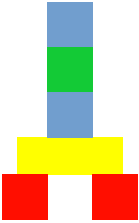
\includegraphics[scale=0.20]{figures/chapter2/task_goal.pdf}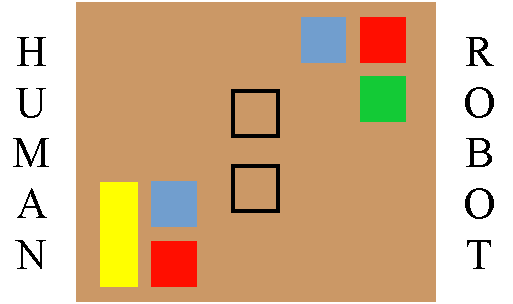
\includegraphics[scale=0.18]{figures/chapter2/task_setup_mini.pdf}}   
	\fancyhead[RO]{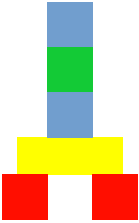
\includegraphics[scale=0.20]{figures/chapter2/task_goal.pdf}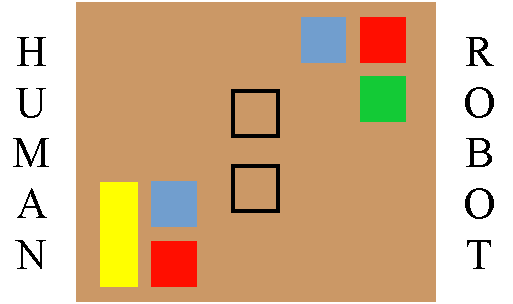
\includegraphics[scale=0.18]{figures/chapter2/task_setup_mini.pdf}\bfseries\thepage}  
	\fancyhead[RE]{\bfseries\nouppercase{\leftmark}}      % Chapter in the right on even pages
	\fancyhead[LO]{\bfseries\nouppercase{\rightmark}}     % Section in the left on odd pages
}%

\usepackage{pdfpages}
\usepackage{makecell}
\usepackage{pdflscape} 
\usepackage{mathtools}
\usepackage[section]{placeins}
\usepackage{afterpage}

%%%%%%%% my commands
\newcommand{\etal}{\textit{et al}.}
\newcommand{\ie}{\textit{i.e.}, }
\newcommand{\eg}{\textit{e.g.}, }
\newcommand{\fact}[3]{\mbox{\textit{#1}(#2, #3)}}
\newcommand{\circledtext}[1]{\raisebox{.5pt}{\textcircled{\raisebox{-.9pt} {#1}}}}
\newcommand{\sparql}{\textsc{SPARQL}}

\newcommand{\algConst}[1]{${\scriptscriptstyle #1}$}
\newcommand{\algNormTextSub}[2]{$\text{#1}_{#2}$}

\newcommand{\aslnumber}[1]{$#1$}
\newcommand{\aslstring}[1]{\textsf{#1}}
\newcommand{\aslvar}[1]{\textcolor{purple}{\textit{#1}}}
\newcommand{\asllabel}[1]{\textbf{#1}}
\newcommand{\annotation}[1]{{\footnotesize #1}}
\newcommand{\rulebody}[1]{\mbox{\hspace{.05\linewidth}}\begin{minipage}[t]{0.9\linewidth}#1.\end{minipage}}
\newcommand{\context}[1]{\begin{minipage}[t]{0.9\linewidth}#1\end{minipage}}
\newcommand{\planbody}[1]{\begin{minipage}[t]{0.9\linewidth}#1.\end{minipage}}
\newcommand{\Jason}[0]{\textbf{\textit{Jason}}}
\newcommand{\sn}{\mbox{\large\textbf{\texttt{\textasciitilde}}}}


\sloppy
\begin{document}
	\setcounter{chapter}{5} %% Numéro du chapitre précédent ;)
	\dominitoc
	\faketableofcontents
	\fi

\chapter{\acrshort{jahrvis} Internal Mechanisms}\label{chapter:chap6}
\minitoc

The objective of this chapter is to present the \acrshort{jahrvis} processes involved in the decision-making and the control of the robot when it is jointly interacting with a human. First, we present the knowledge representations used, then the \acrlong{ism}, the \acrlong{ham}, the Shared Plans Handling composed of two processes, one for the robot (\acrlong{rpm}) and one for the human (\acrlong{hpm}), the \acrlong{aem}, and finally the \acrlong{cm}.

Most of the examples given in this chapter will be based on a collaborative task, the \emph{StackBuildingTask}, which we will now present. It has been inspired by~\cite{devin_2017_decisions}. A human and a robot have to build a block construction together as represented in Figure~\ref{chap6:subfig:task_goal}. At the beginning of the task, the robot and the human have several colored cubes (the yellow one will be referred to as a stick) they can access as in a set-up like the one illustrated in Figure~\ref{chap6:subfig:task_setup}. Two placements are set on the table to indicate where to put the two red cubes which are the base of the stack. Each agent has 3 available actions: Pick, Place and Wait. They can only access to the cube on their side of the table. Figure~\ref{chap6:fig:building_task} is a picture of the task being performed with a human and a PR2 robot. The PR2 robot executes the task fully autonomously, thanks to the robotic architecture presented in Section~\ref{chap3:sec:rob_archi}. A video of the task with the robot running completely autonomously can be seen\footnote{Link to come}.\todo{video}

\begin{figure}[!htb]
%	\centering
	\hspace*{\fill}%
	\subfloat[Goal of the task (side view)]{\label{chap6:subfig:task_goal}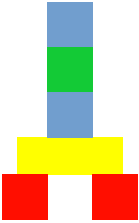
\includegraphics[width=0.2\linewidth]{figures/chapter2/task_goal.pdf}}\hfill
	\subfloat[One initial set-up (top view)]{\label{chap6:subfig:task_setup}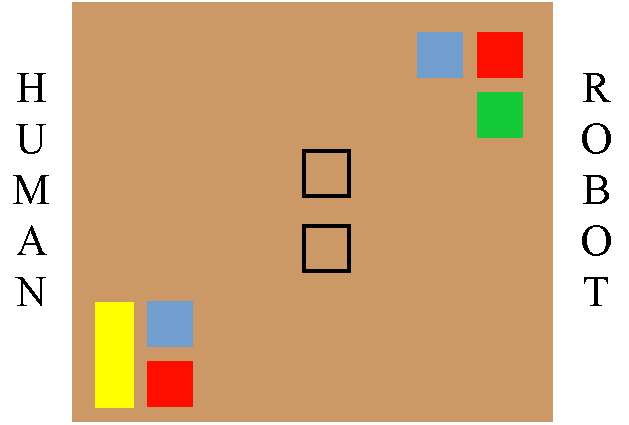
\includegraphics[width=0.5\linewidth]{figures/chapter2/task_setup.pdf}}
	\hspace*{\fill}
	\caption{Description of the blocks building task. The human and the robot have to build the stack together. We assume that the robot and the human know where all the available blocks are. We would like the robot to adapt as much as possible to the human actions and decisions while avoiding useless or tiresome verbal interactions.}
	\label{chap6:fig:task_blocks}
\end{figure}

Figure~\ref{chap6:fig:task_blocks} will be reminded in page headers where the StackBuildingTask example will be mentioned.

\begin{figure}[!ht]
	\centering
	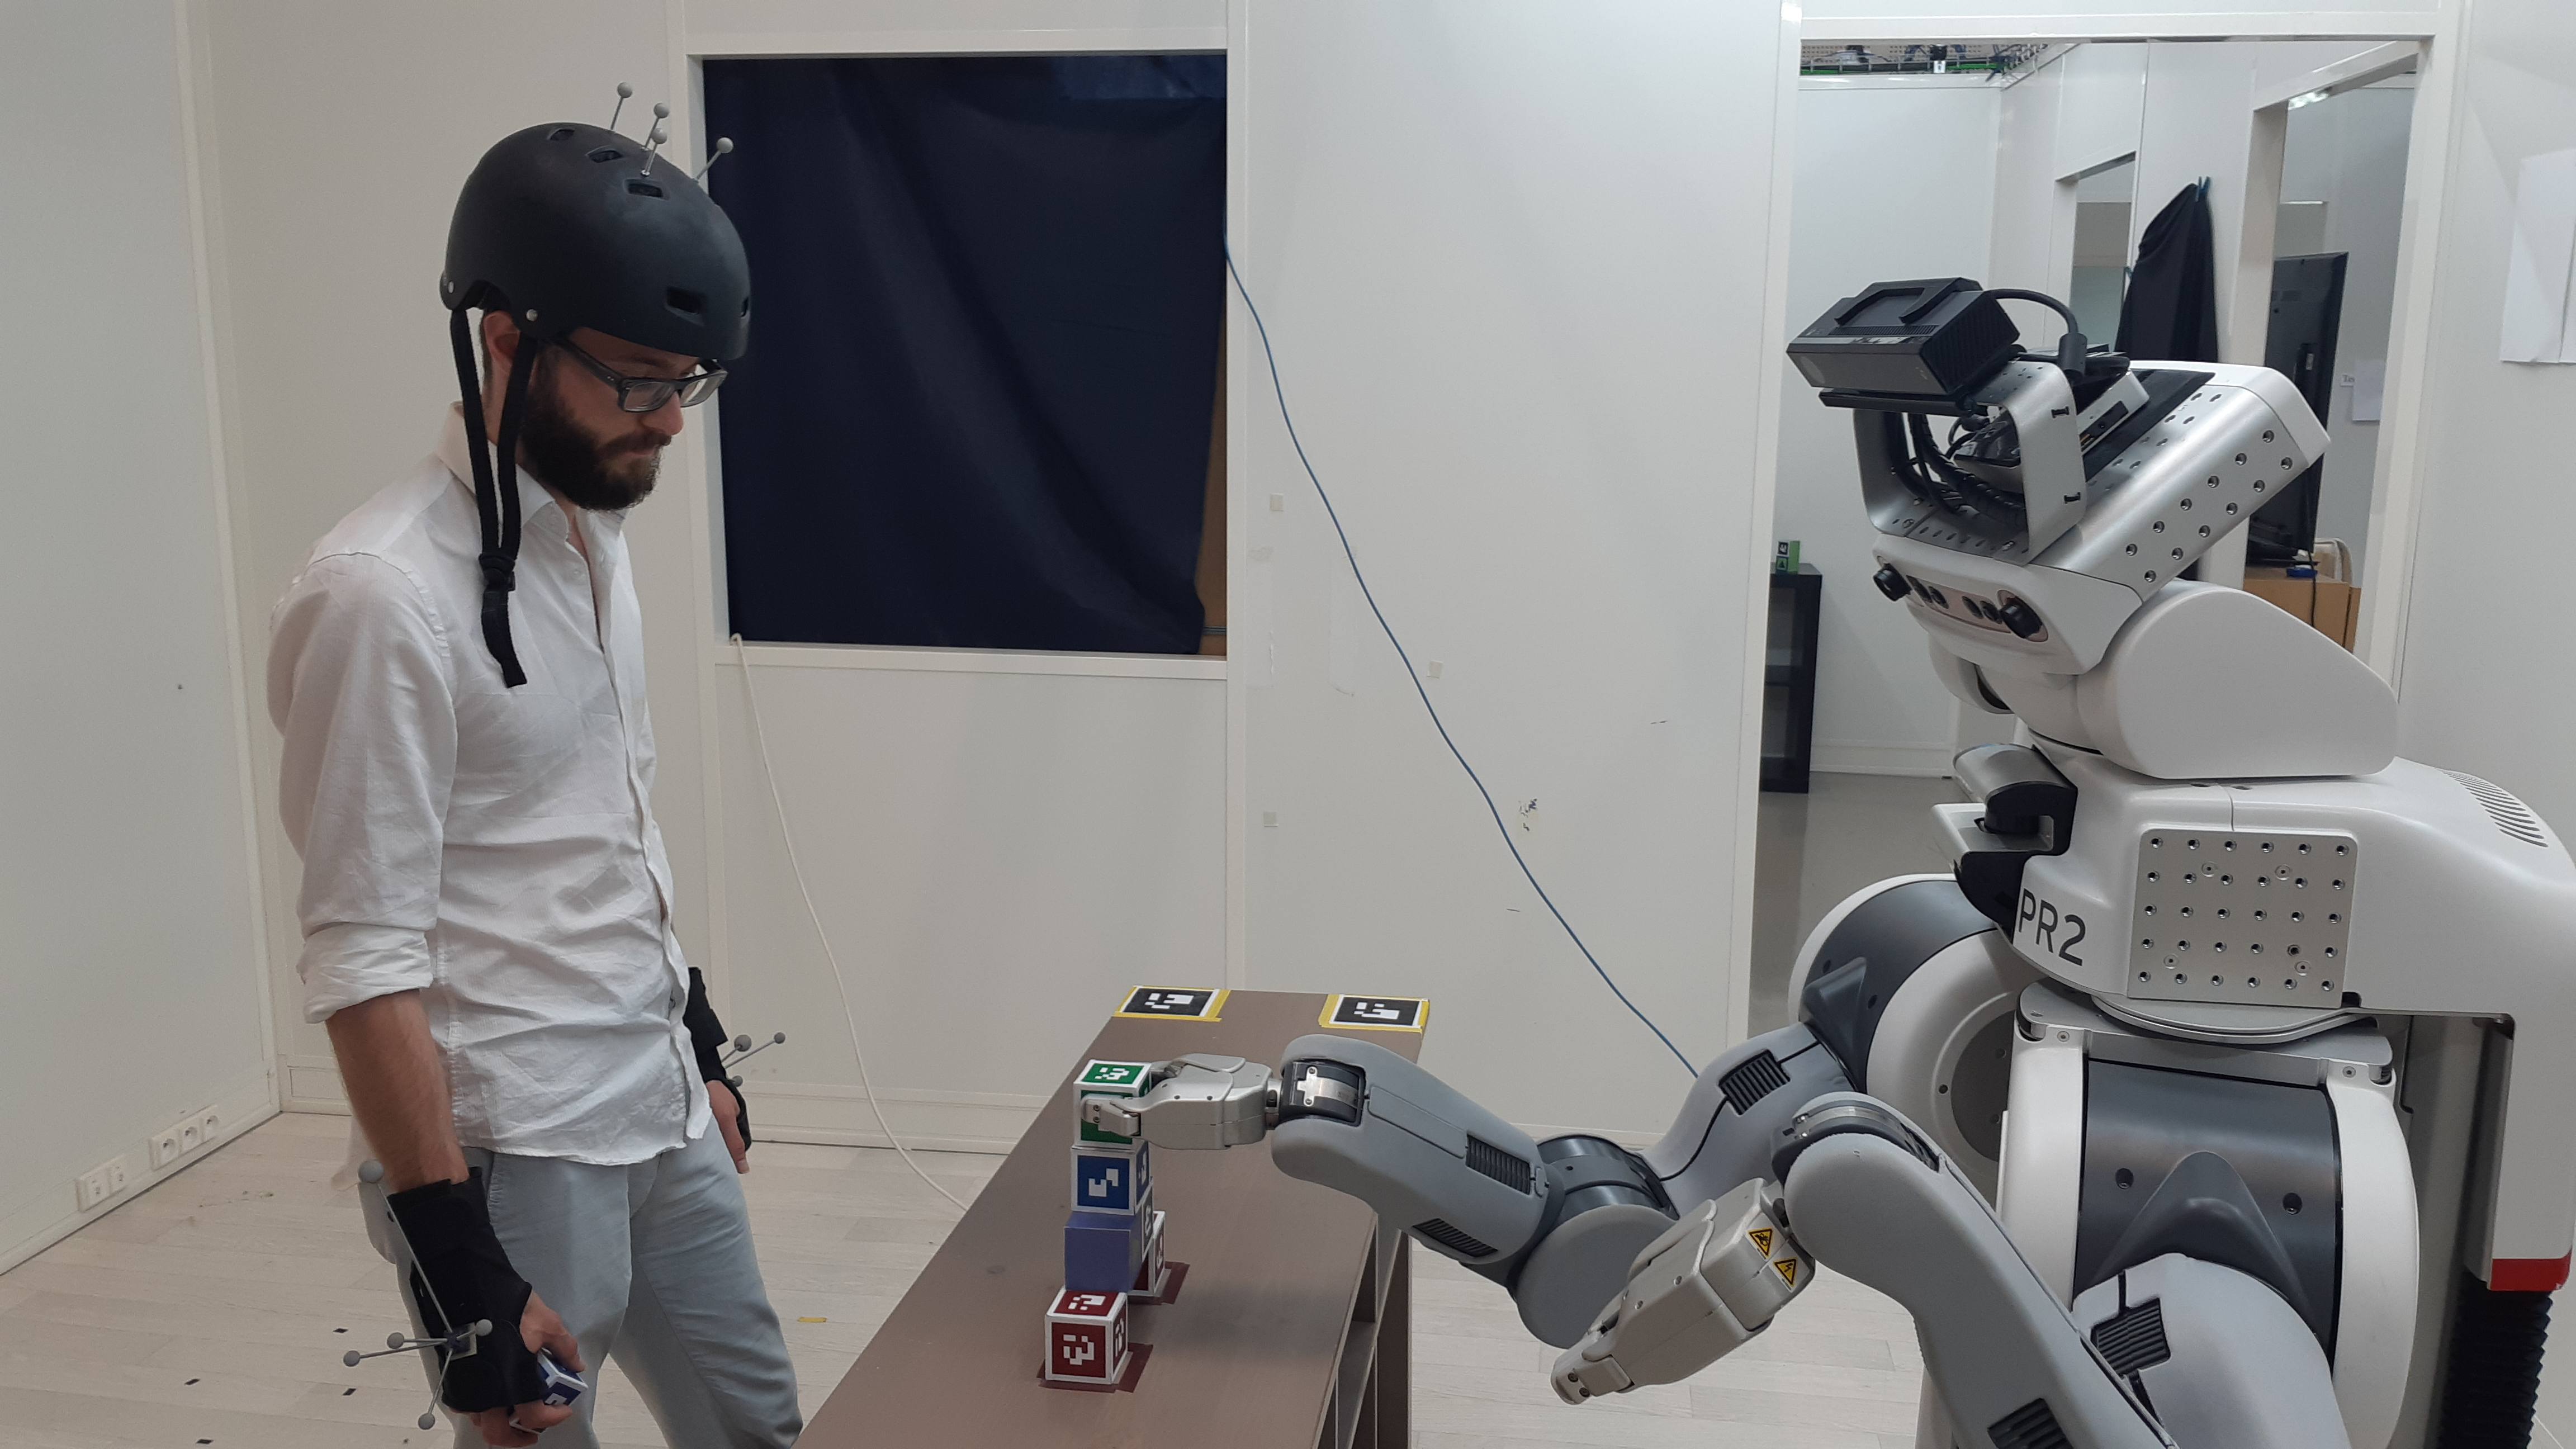
\includegraphics[width=0.7\linewidth]{figures/chapter2/building_task.jpg}
	\caption{The StackBuildingTask being performed by a human and a PR2 robot. The human is perceived through motion capture and the cubes with the Kinect on the robot head.}
	\label{chap6:fig:building_task}
\end{figure}

The task is simple, but still, it involves both agents which will have to collaborate, and there are potential conflicts and decisions to take into account. It brings situations where the robot has to adapt to the human's needs and preferences.

\section{Knowledge Representations and Management}\label{chap6:sec:know}
As shown in Section~\ref{chap1:subsubsec:shared_rep} and Section~\ref{chap1:subsubsec:common_g}, when involved in joint actions, humans maintain shared representations of tasks, actions, goals and have a common ground. Thus, it is important that the robot has such representations.

During an interaction, \acrshort{jahrvis} processes use Knowledge Bases (KB) of two types: internal and external ones. Concerning the first type, each \acrshort{rja} has its own knowledge base that is called belief base in Jason vocabulary. It is used for knowledge which serves to \acrshort{jahrvis} internal computations only. As for the external knowledge bases, there are the ones presented in Section~\ref{chap3:subsubsec:kb} as part of the robotic architecture, Ontologenius and Mementar. Updates from subscription to Ontologenius facts are received through ROS topics and converted as Jason percepts to be added to the subscribing \acrshort{rja} belief base. 

Table~\ref{chap6:tab:data} shows a description of the data circulating between the \acrshort{jahrvis} \acrshort{rja}s and the 2 \acrlong{kb}s, Ontologenius and Mementar.

\begin{landscape}
\begin{table}[]
	\centering
	\begin{tabular}{p{0.34\textwidth}||p{0.39\textwidth}|p{0.43\textwidth}|p{0.2\textwidth}|}
		
		&
		\acrshort{rja} subscription to \acrshort{kb}&
		\acrshort{rja} request/\acrshort{kb} response &
		\acrshort{rja} feeding \acrshort{kb} \\ \hline\hline
		
		\acrlong{ism} &
		\fact{isEngagedWith}{Human}{Robot}\newline
		\fact{isPerceiving}{Robot}{Human}\newline 
		\fact{isLookingAt}{Human}{Robot} &
		 &
		Start and end of interaction sessions \\ \hline
		
		\acrlong{rpm} &
		\fact{isLookingAt}{Human}{Robot} &
		Class of actions\newline SPARQL $\rightarrow$ Object &
		Start and end of abstract tasks \\ \hline
		
		\acrlong{hpm} &
		\fact{isPerceiving}{Human}{Robot}\newline \fact{isPerceiving}{Robot}{Human}\newline \fact{isLookingAt}{Human}{Robot}\newline \fact{isLookingAt}{Human}{Object} &
		Class of actions\newline Existence of action effects\newline SPARQL $\rightarrow$ Object &
		Start and end of primitive tasks \\ \hline
		
		\acrlong{cm} &
		\fact{isPerceiving}{Robot}{Human} &
		Verb conjugation\newline Class of actions and objects\newline Labels of actions and objects\newline Existence of verbalization contexts &
		\\ \hline
		
		\acrlong{ham} &
		Movements of the human action model\newline Progression effects of the human action model\newline Necessary effects of the human action model &
		Class of Objects\newline Existence of preconditions\newline Existence of isReachable(Object) &
		\\ \hline
		
		\acrlong{aem} &
		&
		Class of actions &
		Start and end of primitive tasks \\ \hline
		
	\end{tabular}
	\caption{Data circulating between the Knowledge Bases (Ontologenius and Mementar) and the \acrshort{jahrvis} \acrshort{rja}s. Data in italics are not task-dependent, the other ones are. The types of the latter are loaded from the action models described in Paragraph:~\nameref{chap6:par:act_rep}. For example, the \acrlong{ham} gets from the internal action model that \fact{handMovingToward}{Human}{Pickable} is a movement of the Pick action. Then, it can subscribe to the updates about this fact type to Ontologenius when a task where the human has a Pick action is ongoing.}
	\label{chap6:tab:data}
\end{table}
\end{landscape}

\subsection{Action Representations}\label{chap6:subsec:action_rep}
Action representations allow 
\begin{bulletList}
	\item the robot to recognize human actions
	\item to execute actions
	\item to monitor the human's attention towards its actions and to communicate about them
\end{bulletList} 

We defined three action representations according to these three uses. Actions should be written and loaded by the programmer according to the task they need the robot to perform, following the defined formats in the dedicated files. This allows \acrshort{jahrvis} core to be task-independent.

Human actions to recognize and robot actions to execute are written in an ASL file to benefit from Jason reasoning features. And, the same actions but with other information allowing \acrshort{jahrvis} to communicate about them and to monitor the human's attention towards them are stored in Ontologenius to benefit from the reasoning features. This latter representation is described in the next paragraph.

\paragraph{External Action Representation} (\ie stored in Ontologenius).
For the needs of \acrshort{jahrvis}, we represented actions, their verbal labels and their effects in the semantic \acrshort{kb} managed by Ontologenius. We show in Figure~\ref{chap6:fig:class_actions} a representation of some actions we stored in Ontologenius using the Web Ontology Language (OWL) (see Listing~\ref{chap2:lst:classes}) and in Figure~\ref{chap6:fig:class_effects} a representation of possible action effects.

\begin{lstlisting}[style=OwlTurtle, label={chap2:lst:classes}, caption={Description of ontology classes in the OWL language using the Turtle syntax.} ]
:PhysicalAction	rdf:type owl:Class ;
				rdfs:subClassOf :HtnAction .

:PlaceAction	rdf:type owl:Class ;
			rdfs:subClassOf :PhysicalAction ;
			htn_actions:hasEffect :IsOnTopOfEffect ;
			rdfs:label ``{Agent} @Place {Pickable}'' .

\end{lstlisting}

One of the advantages of using action model stored in Ontologenius is the class inheritance. It allows to define properties for one class that will be transmitted to its child classes (\eg if it exists multiple class representing a Place action, let's say \verb'human_place_cube' and \verb'robot_place_cube', both inherit from the properties of \verb'PlaceAction' such as the label used for the action verbalization). Another advantage is to be able to link classes through properties and to easily query the \acrshort{kb} about it (\eg what are the effects of the \verb'PickAction' and then what types of effects are they?).

\begin{figure}[!ht]
	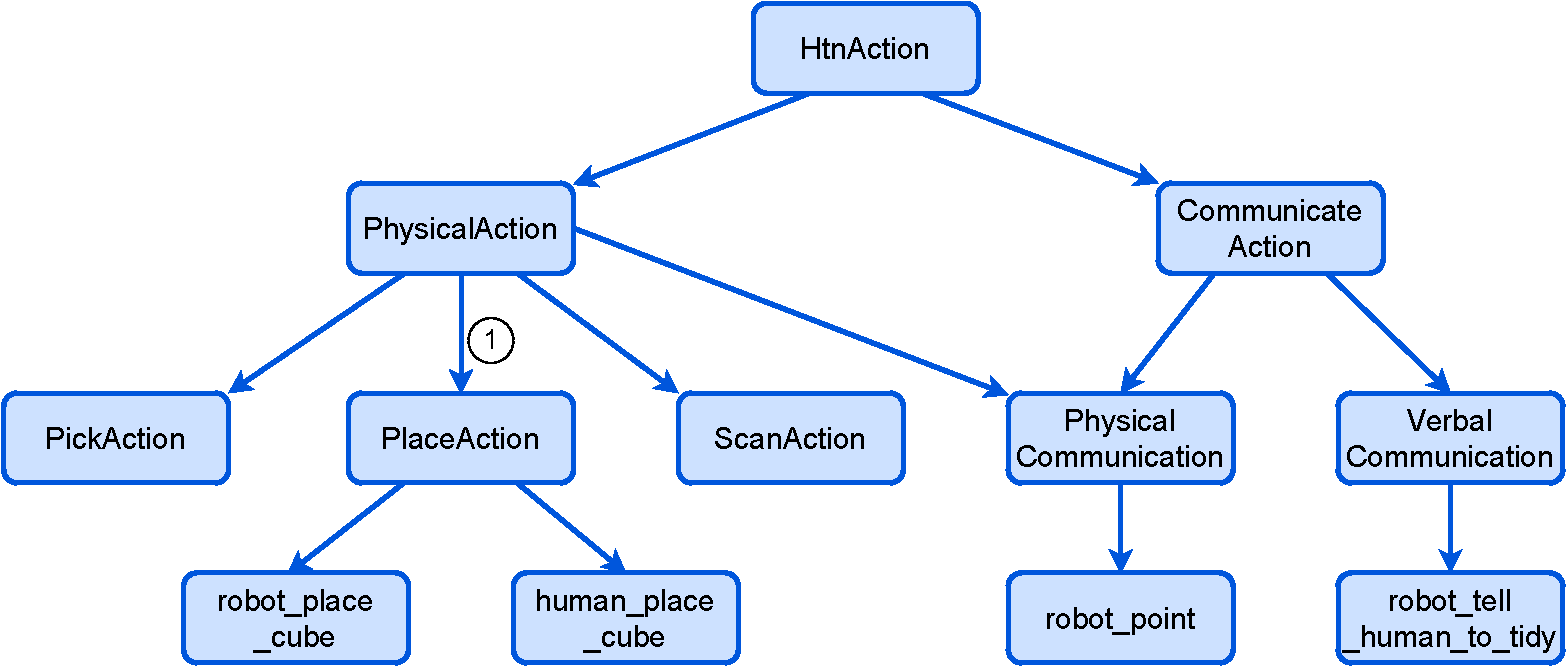
\includegraphics[width=\linewidth]{figures/chapter2/class_actions.pdf}
	\caption{The representation of an extract of the ontology class hierarchy graph of \acrshort{htn} actions. Taking the class PhysicalAction, the arrow \circledtext{1} has to be read	as \textit{``A PlaceAction is a kind of PhysicalAction''}.}
	\label{chap6:fig:class_actions}
\end{figure}

\begin{figure}[!ht]
	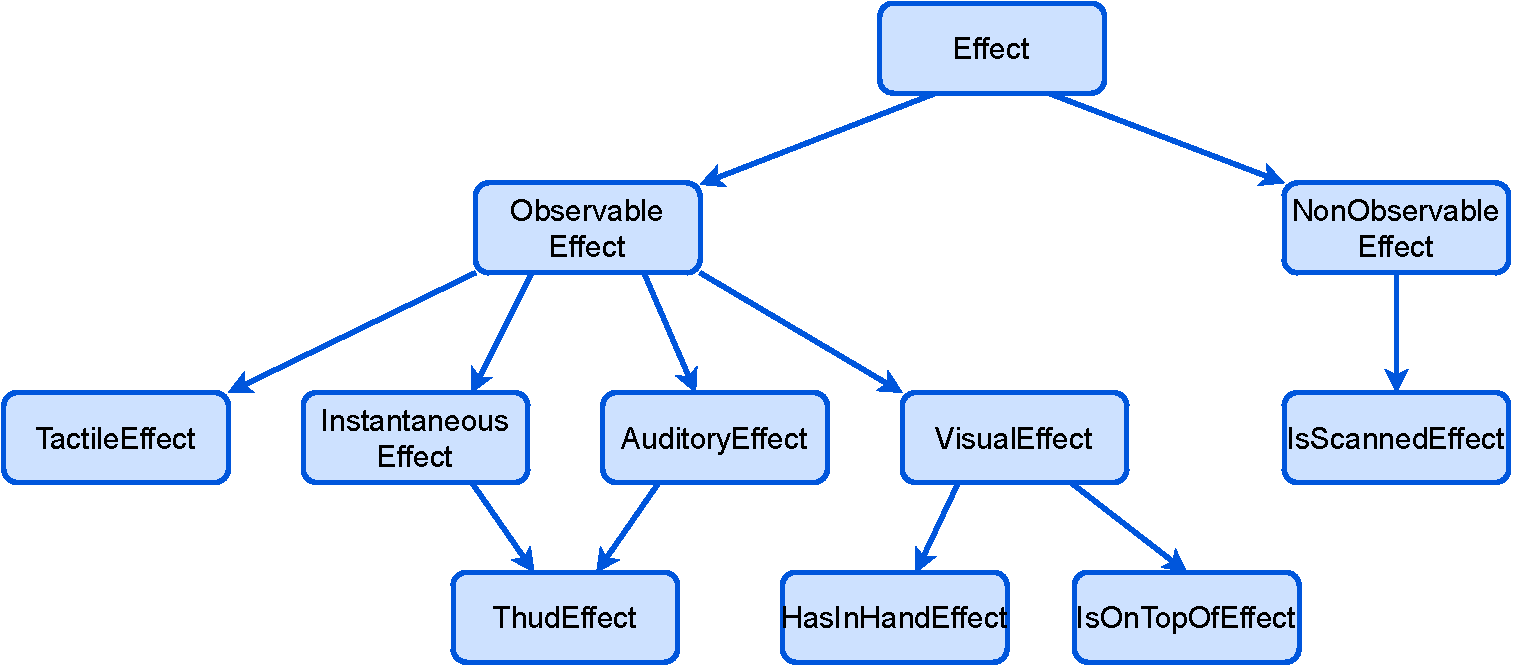
\includegraphics[width=\linewidth]{figures/chapter2/class_effects.pdf}
	\caption{The representation of an extract of the ontology class hierarchy graph of action effects. Taking the class ThudEffect, the arrows \circledtext{1} and \circledtext{2} indicate that ThudEffect is and an InstantaneousEffect and an AuditoryEffect.}
	\label{chap6:fig:class_effects}
\end{figure}

As we know, when an agent performs an action, the other agent may monitor it, if present, in order to follow the task progress and to know when the action is over. A way to know that an action is over is to check if the action effects has been added to the current worldstate or not. Such a mechanism is used by the \acrlong{hpm} as explained in Section~\ref{chap6:subsec:human_plan}. However, effects may be perceived differently according to the agent type as humans and robots does not have the same perception modalities (and even in one given type it can differ). In Figure~\ref{chap6:fig:class_effects}, we represented a possible way to model and classify action effects. And so, because Ontologenius is designed for \acrshort{hri}, it is possible to have different representations for robot agents and human agents. We present now a use case with its illustration in Figure~\ref{chap6:fig:kettle}. An agent may have to perform \verb'HeatWaterInKettleAction'. If it is performed by the human, the robot has to monitor the action effects to know if the action is over or not. However, a robot is not able to observe that a kettle has finished to boil water, thus the action has a non-observable effect for the robot. Then, probably the robot will ask the human if the action is over or will see that the human performs its next action of the plan. Now, if we place ourselves in the case where the robot is the one performing the action -- with a smart kettle --, it wants to check if the human could be aware of the action end (because if they are not aware, it should inform them). The criteria \acrshort{jahrvis} takes into account is, was the effect observable by the human partner? To answer this question, it first needs to know what the observable effects of \verb'HeatWaterInKettleAction' for the human (if there are). Then, it can query the human's belief base in Ontologenius and get the knowledge that for them, the effect of \verb'HeatWaterInKettleAction' belongs to the class \verb'ThudEffect' (when the kettle stops, it produces a thud) and \verb'TactileEffect' (when the kettle boils water, it becomes hot).
	
\begin{figure}[!ht]
	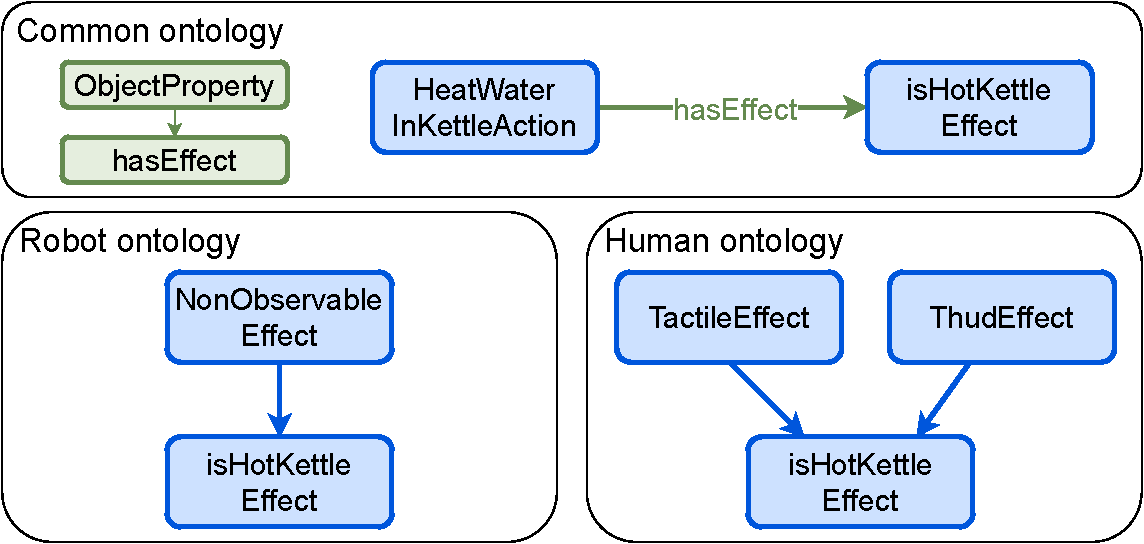
\includegraphics[width=\linewidth]{figures/chapter2/kettle.pdf}
	\caption{Illustration of the human and the robot having differing ontologies. Both have the common knowledge that HeatWaterInKettleAction has isHotKettleEffect as effect. However, in the robot ontology, isHotKettleEffect is defined as a NonObservableEffect whereas in the estimated human ontology it is defined as a TactileEffect and a ThudEffect which are both ObservableEffect as shown in Figure~\ref{chap6:fig:class_effects}.}
	\label{chap6:fig:kettle}
\end{figure}

Finally, as mentioned earlier and as visible in Listing~\ref{chap2:lst:classes}, Ontologenius allows to define label classes and so label for actions. These labels are then used by \acrshort{jahrvis} to verbalize the plan actions and based on a simple grammar we defined. For example, in ``\{Agent\} @Place \{Pickable\}'', elements between braces are to be instantiated at execution time by \acrshort{jahrvis} communication process when needed. Then, the @ symbol indicates that the word is a verb that should be conjugated. Verb conjugations can also be found in the \acrshort{kb} as shown in Listing~\ref{chap2:lst:verb}. Thus, the communication manager could process it leading to ``I placed the blue cube''.

\newpage

\begin{lstlisting}[style=OwlTurtle, label={chap2:lst:verb}, caption={Description of the class describing the verb Place in the third-person present-tense, in the OWL language using the Turtle syntax.} ]
:PlaceTSPSimplePresent	rdf:type owl:Class ;
						rdfs:subClassOf :PlaceSimplePresent ;
						rdfs:subClassOf :ThirdSingularPersonalForm ;
						rdfs:label ``place''@fr ;
						rdfs:label ``places''@en .
\end{lstlisting}

We have seen the possibilities offered by Ontologenius to \acrshort{jahrvis}. Now, we present the two internal action representations, one of the human actions in order to recognize them and the other one is of the robot actions, to allow the robot to estimate the human monitoring activity of its actions. 

\paragraph{Internal Action Representation}\label{chap6:par:act_rep}(\ie stored in \acrshort{jahrvis})\mbox{}

\bigskip
What does \acrshort{jahrvis} need to \textbf{recognize a human action}? We defined a human action as: 
\[Act_H=\langle Action,PrecondL,MoveL,ProgEffectL,NecessEffectL\rangle\] where $Action$ is a predicate in the form of a triplet $ActName(Agent,Params)$ with $ActName$ the action name, $Agent$ the class of the agent performing it (\eg Human or Worker) and $Params$ a list of the action parameter classes; $PrecondL$ the list of the action preconditions; $MoveL$ the list of distinctive movements that the human could do when performing the action; $ProgEffectL$ the list of effects that we coined \textit{progression effects} which are action effects, not enough to rule the action end but allowing the plan managers to estimate that an action is progressing towards its end; and $NecessEffectL$ the list of effects that we coined \textit{necessary effects} which are action effects existing iff the action is over.

Our action model takes the form of Jason beliefs written in an ASL file, added as input of the \acrshort{rja} \acrlong{ham}. For example, the actions Pick and Place for a human are represented as:
\begin{lstlisting}[style=aslDef]
actionModel(pick(Human,[Pickable]),
			[isOnTopOf(Pickable,Support)],
			[handMovingToward(Human,PickableList)],
			[isHolding(Human,Pickable)],
			[~isOnTopOf(Pickable,Support)]).

actionModel(place(Human,[Pickable,Support]),
			[isHolding(Human,Pickable)],
			[handMovingToward(Human,SupportList)],
			[~isHolding(Human,Pickable)],
			[isOnTopOf(Pickable,Support)]).
\end{lstlisting}

The choice to have two kinds of effects has been made in order to allow the \acrlong{ham} to be robust to a potentially unreliable perception. Indeed, for example in the case of a Place action, the perception of an object hold by a human can be jumpy, multiple addition/deletion of the fact \fact{isHolding}{human\_0}{blue\_cube\_1}. But, if the robot perceives that the object has been placed on top of a support, it can assume that the action is really over. The algorithm of the \acrlong{ham} will be more detailed in Section~\ref{chap6:sec:h_moni}.

\bigskip

The action representation for \textbf{robot action execution} allows to match, for a given action, its name and the motion planner and executor needed to execute it. It is possible to specify how the action parameter should be fed to the motion planner and the reaction the robot should have in case of execution failure. The example given in Listing~\ref{chap6:listing:int_rep_act_exec} shows what functions of the motion planner and executor call and how the system should react in case of failure.
\begin{lstlisting}[label=chap6:listing:int_rep_act_exec,style=aslDef, frame=single, caption={Example of an internal action definition for a robot action. The first Jason plan specifies what function to call to execute the Place action. The second plan describes what should be done in case of action planning or execution failure. The third plan is triggered when the first plan has already been tried twice and was requested for a third time. In this case, the failure is signaled at the plan level.}]
// execution limited to 2 trials in a raw
@place[max_attempts(2)] 
+!place(Params) : planPick("armUsed", Arm) <-
			.nth(1, Params, Obj);
			headManager(Obj,environment_monitoring,urgent);
			planPlace(Obj, Arm);
			execute("place").
		
// in case of failure, we try again if did not already
-!place(Params)[error_msg(Msg)] : 
	not .substring(max_attempts,Msg) <-
			+error_msg(Msg);
			!place(Params).

// if we tried to execute the plan three times in a raw,
// the action is dropped	 
-!place(Params)[error_msg(Msg)] : 
	.substring(max_attempts,Msg) <-
			?error_msg(Msg);
			.fail_goal(executeAction,[error_msg(Msg)]).
\end{lstlisting}


\subsection{Shared Plan Representation}\label{chap6:subsec:shared_p_rep}
As explained in Section~\ref{chap5:sec:levels}, we represent shared plans using \acrfull{htn} as \acrshort{hatp} and \acrshort{hatpehda}, the planners we use generate \acrshort{htn}-based plans. This formalism allows to deal with goal-based and situation-based activities at different levels of hierarchy such as task, subtasks -- abstract tasks using planning vocabulary -- and actions -- atomic, primitive tasks -- and consequently to consider different levels of granularity. For example, it may be useful to \acrshort{jahrvis} to be able to request a plan for a given abstract task which failed\footnote{This is future work.}. Another advantage is that it is easy then for the robot to communicate about subtasks and not only about actions without context. However, according to the task or the domain, the \acrshort{htn} expressiveness for this matter raises discussion. Indeed, \acrshort{htn} plans often make use of recursive abstract tasks which becomes useless for replanning because such abstract tasks have no semantic meaning. Indeed, if we take the piece of plan presented in Figure~\ref{chap6:fig:recursive_task}, to communicate to the human that the abstract task PlaceAllObjects has failed does not give a information precise enough since there are several of them.

\begin{figure}[!ht]
	\centering
	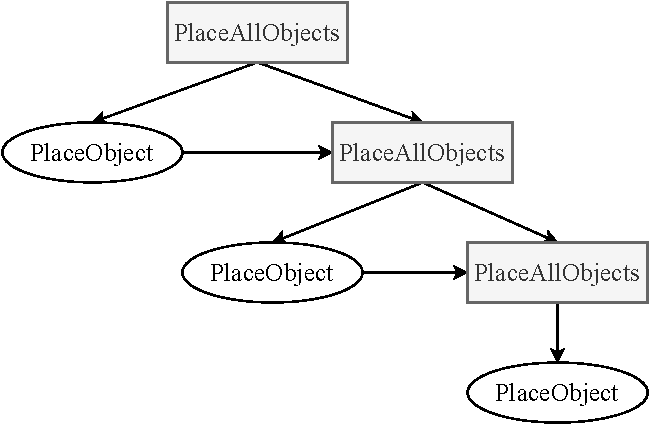
\includegraphics[width=0.6\linewidth]{figures/chapter2/recursive_task.pdf}
	\caption{Example of a recursive abstract task. The white ellipses correspond to primitive tasks while gray rectangles represent abstract ones.}
	\label{chap6:fig:recursive_task}
\end{figure}

Moreover, in the next section (see~\ref{chap6:subsec:feeding}), we show how \acrshort{jahrvis} feeds the episodic ontology, a timeline, with abstract and primitive task executions. It becomes humanly unreadable with recursive tasks. A concept such as the ``iterative task'' proposed by \cite{martinie_2011_structuring} would be interesting if used in a \acrshort{htn} plan for \acrshort{hri}. However, there is currently no such thing, so when manipulating such plans, we have two modalities:
\begin{enumerate}
	\item the domain is written being aware of this issue and thus, \acrshort{jahrvis} takes abstract tasks as input besides primitive tasks (\ie in the current work, plans generated by \acrshort{hatpehda}\footnote{Based on domains intentionally written without recursive tasks by Guilhem Buisan.})
	\item the domain is written with recursive abstract tasks and thus, \acrshort{jahrvis} only selects primitive tasks as tasks being part of the plan (\ie in the current work, plans generated by \acrshort{hatp}\footnote{Reuse of domains written by Sandra Devin.})
\end{enumerate}

We define a shared plan as a sequence of primitive tasks having to be performed by an agent and, abstract tasks. An abstract task $\lambda$ is defined as: 
\[\lambda=\langle id_\lambda,state_\lambda,name_\lambda,\Delta_\lambda\rangle\] 
where $id_\lambda$ is an identification number (id) proper to $\lambda$, $state_\lambda$ is the task state estimated by the robot, $name_\lambda$ is the name of the task and the decomposition id $\Delta_\lambda=id_{\lambda\prime}$ with $id_{\lambda\prime}$ the id of the abstract task $\lambda\prime$ that has been decomposed into other tasks, including $\lambda$.

And, a primitive task $\Pi$ is defined as:
\[\Pi=\langle id_\Pi,state_\Pi,name_\Pi,agent_\Pi,params_\Pi,preds_\Pi,\Delta_\Pi\rangle\]

where $id_\Pi$ is an id proper to $\Pi$, $state_\Pi$ is the task state estimation by the robot, $name_\Pi$ is the name of the task, $agent_\Pi$ is the name of the agent that should perform the task, $params_\Pi$ is the list of parameters required for the task execution, $preds_\Pi={id_{\Pi\prime},...,id_{\Pi\prime\prime}}$ the list of ids of the tasks $\Pi\prime,...,\Pi\prime\prime$ needing to be achieved before the task $\Pi$ can start, and the decomposition id $\Delta_\Pi=id_{\lambda}$ with $id_{\lambda}$ the id of the abstract task $\lambda$ that has been decomposed into other tasks, including $\Pi$.

We defined nine possible values for an abstract or primitive task $state$ which are shown in Table~\ref{chap6:tab:task_states}. 

\begin{table}[h]
	\centering
	\begin{tabular}{l|l}
		State            & Description         \\\hline\hline
		\textsc{planned} & needs to be done later        \\
		\textsc{todo}            & needs to be done now   \\
		\textsc{ongoing}          & is in progress       \\
		\textsc{executed}         & is achieved               \\
		\textsc{suspended}        & needs to be set to \textsc{unplanned}\\ 
		\textsc{unplanned} & is not part of the plan anymore (used with conditional plans) \\
		\textsc{not\_starting}    & was \textsc{todo} but took to much time before starting \\
		\textsc{not\_finished}     & was started but has not been achieved    \\
		\textsc{not\_seen}         & was achieved but has not been observed by the other agent    
	\end{tabular}
	\caption{The nine possible state values of an abstract or primitive task.}
	\label{chap6:tab:task_states}
\end{table}

So, for example, an excerpt of the StackBuildingTask plan in which the human and the robot place the first blue cube of the stack and the green cube, generated by \acrshort{hatpehda} and represented in Figure~\ref{chap6:fig:excerpt_plan}, is:
\thispagestyle{example}
\begin{align*}
&\lambda_{13}=\langle 13,\textsc{Planned},\text{h\_place\_blue\_cube},1\rangle \\
&\lambda_{4}=\langle 4,\textsc{Planned},\text{r\_place\_green\_cube},1\rangle \\
&\Pi_{139}=\langle 139,\textsc{Planned},\text{human\_place\_cube},\text{human\_0}, [\text{blue\_cube\_2,stick}],138,13\rangle \\
&\Pi_{141}=\langle 141,\textsc{Planned},\text{robot\_place\_cube},\text{pr2\_robot},[\text{green\_cube,blue\_cube\_2}], &\\  & &139,4\rangle
\end{align*}\todo{arrange}

\begin{figure}[!ht]
	\centering
	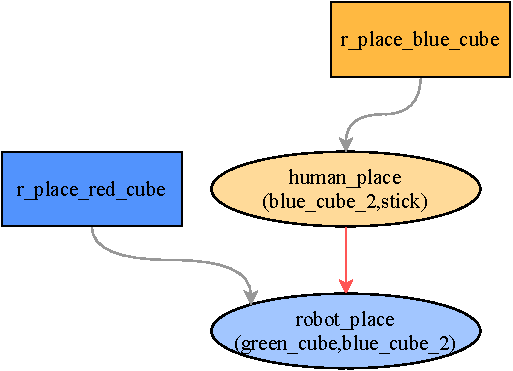
\includegraphics[width=0.5\linewidth]{figures/chapter2/excerpt_plan.pdf}
	\caption{An excerpt of the StackBuildingTask plan. The ellipses correspond to primitive tasks while rectangles represent abstract ones. The blue shapes are robot tasks and the yellow ones are the human ones. Finally, red arrows indicate the sequence of actions in the plans and gray ones represent hierarchical links, \textit{i.e.}~the links between the tasks as defined in the \acrshortpl{htn}.}
	\label{chap6:fig:excerpt_plan}
\end{figure}

\subsection{Feeding the Knowledge Base}\label{chap6:subsec:feeding}
Until now, we stayed focused on semantic knowledge going from the external \acrshort{kb} to \acrshort{jahrvis}. But, as mentioned earlier, one of the external \acrshort{kb} is dedicated to episodic knowledge. This \acrshort{kb} takes the form of a timeline, managed by Mementar. Whereas Ontologenius feeds \acrshort{jahrvis} with knowledge, the flow is inverted for the episodic data, as Mementar is fed by \acrshort{jahrvis} among other components. Indeed, when an abstract or primitive task is started or achieved, this information is sent to Mementar for storage with the associated ID and time stamp. The objective is to have a history of the task proceeding. One of the possible uses of such a history is for the robot to refer to past events during a task when communicating.
Moreover, \acrshort{jahrvis} adds the semantic data associated to a task -- agent and parameters -- to the semantic ontology. 
%We illustrate the timeline in Figure~\ref{chap6:fig:timeline} with the same example as the one above for the plan, one cube is placed by each agent.


%\begin{figure}[!ht]
%	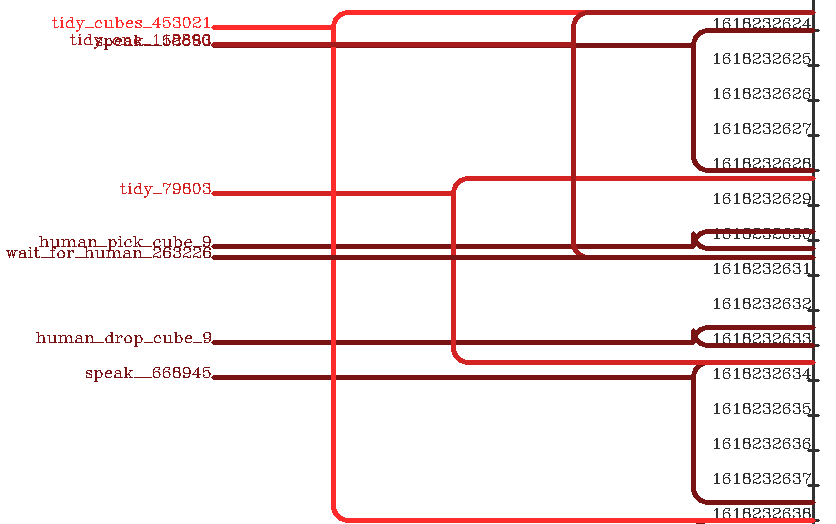
\includegraphics[width=\linewidth]{figures/chapter2/timeline.png}
%	\caption{Piece of timeline of an executed StackBuildingTask plan where the robot and the human had to place a cube each. It has been generated by Mementar after having received data from \acrshort{jahrvis}.}
%	\label{chap6:fig:timeline}
%\end{figure}\todo{refaire et ajouter le temps en legende}


\thispagestyle{example}

\section{Interaction Session Management} 

\begin{figure}[!htb]
	\centering
	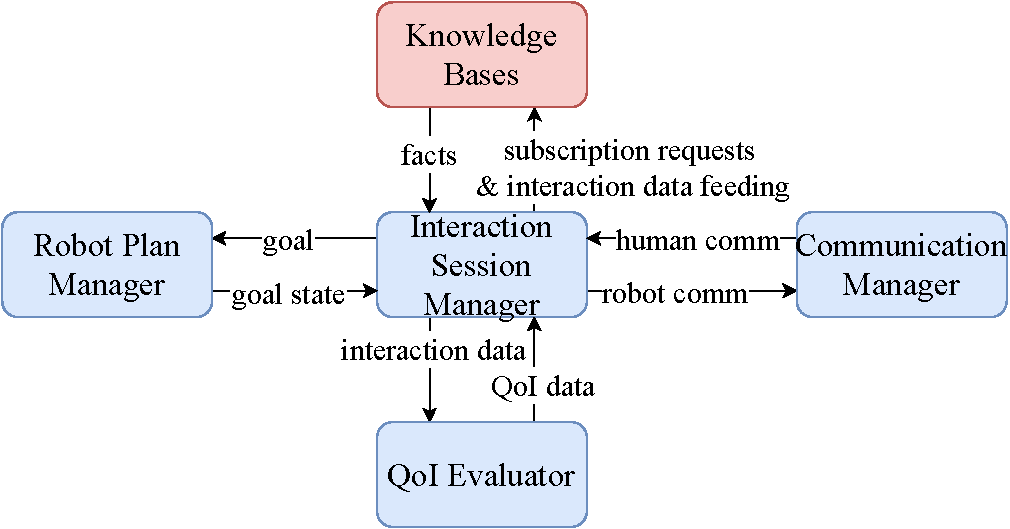
\includegraphics[width=0.7\linewidth]{figures/chapter2/session_manager_zoom.pdf}
	\caption{The \acrlong{ism} and the \acrshort{rja}s (in blue) and the component of the robotic architecture (in red) with which it interacts.}
	\label{chap6:fig:session_manager_zoom}
\end{figure}

The \acrfull{ism} handles the interaction sessions and manages the robot (shared) goals. Figure~\ref{chap6:fig:session_manager_zoom} proposes a focus on the \acrshort{jahrvis} structure and the components of the robotic architecture around the \acrshort{ism}. Figure~\ref{chap6:fig:session_manager} shows the process we designed, modeling the different states in which the robot can be. Moreover, we thought the manager with the ability to consider that a human can join another one during a conversation. However, we have not implemented it yet.

\begin{figure}[!htb]
	\centering
	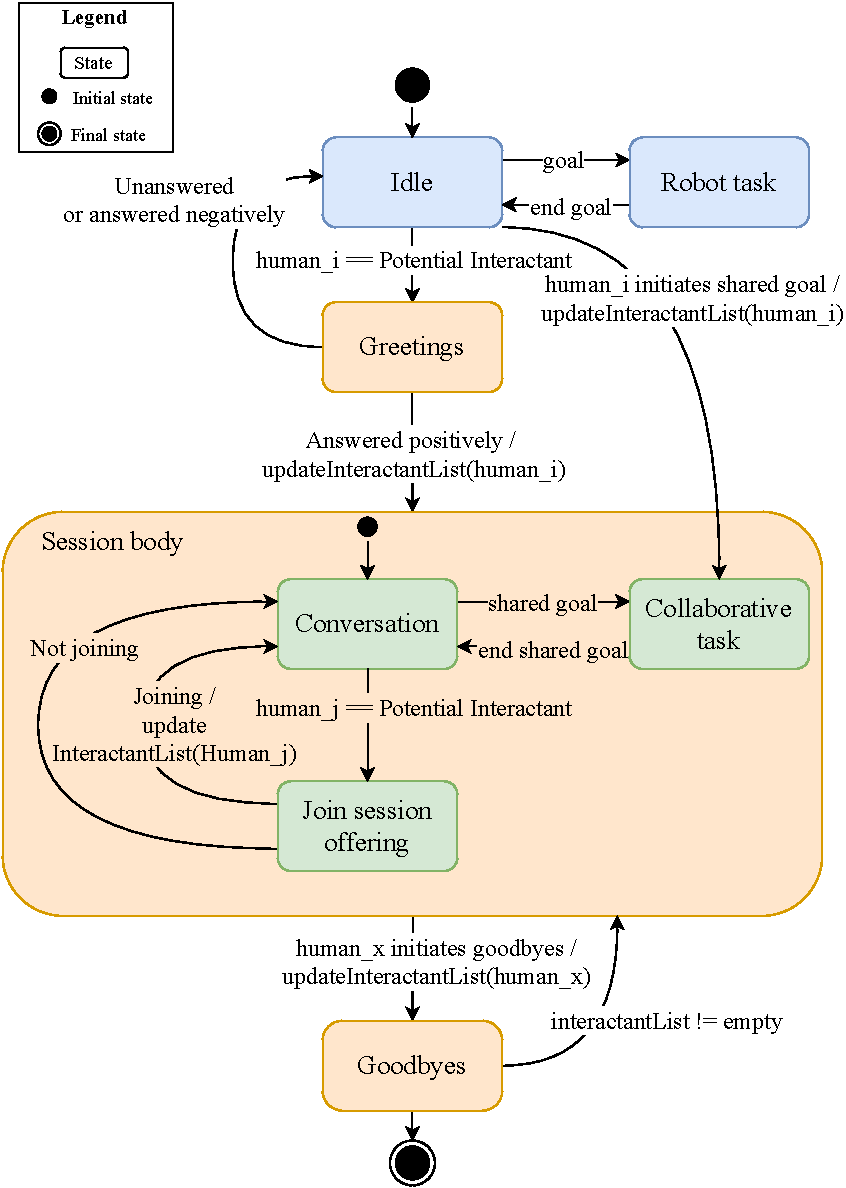
\includegraphics[width=0.8\linewidth]{figures/chapter2/session_manager.pdf}
	\caption{States of the \acrfull{ism}. In blue are represented the states of the \acrshort{ism} when the robot is not in an interaction session. In orange are the states in which the \acrshort{ism} can be during an interaction session. In green are the sub-states of the interaction session body.}
	\label{chap6:fig:session_manager}
\end{figure}

A simpler version works as following. An interaction session is triggered when a human is close enough to start a conversation and seems willing to, \ie when the fact  \fact{isEngagedWith}{human\_i}{robot} is added to the knowledge base and sent to \acrshort{jahrvis}. In this way, the robot tries to respect people that does not want to interact with it. From there, the robot is in the first phase of the interaction session, the \textit{greetings}. The robot says hello to the human and announces the activities it can perform with them, depending on the context they are in. The interaction manager triggers the tracking of the human's head by the robot head. This has two purposes: to signal the robot's engagement and to monitor the human's actions. This behavior is quite similar to the one described by \cite{satake_2015_should}. 


An interaction session stays open as long as the human and the robot perform activities together, \ie as long as the human is engaged in the interaction. This engagement is monitored by the robot in different ways: through the predicate \fact{isEngagedWith}{human\_i}{robot} during dialogue phases outside a task and through what is happening during a task. If at some point the human is not perceived for a while or the human says goodbye, then the manager ends the session. In the latter case, the robot replies with goodbyes. Finally, it returns to its home-base if it has one.

\section{Human Actions Recognition}\label{chap6:sec:h_moni}
\begin{figure}[!hbt]
	\centering
	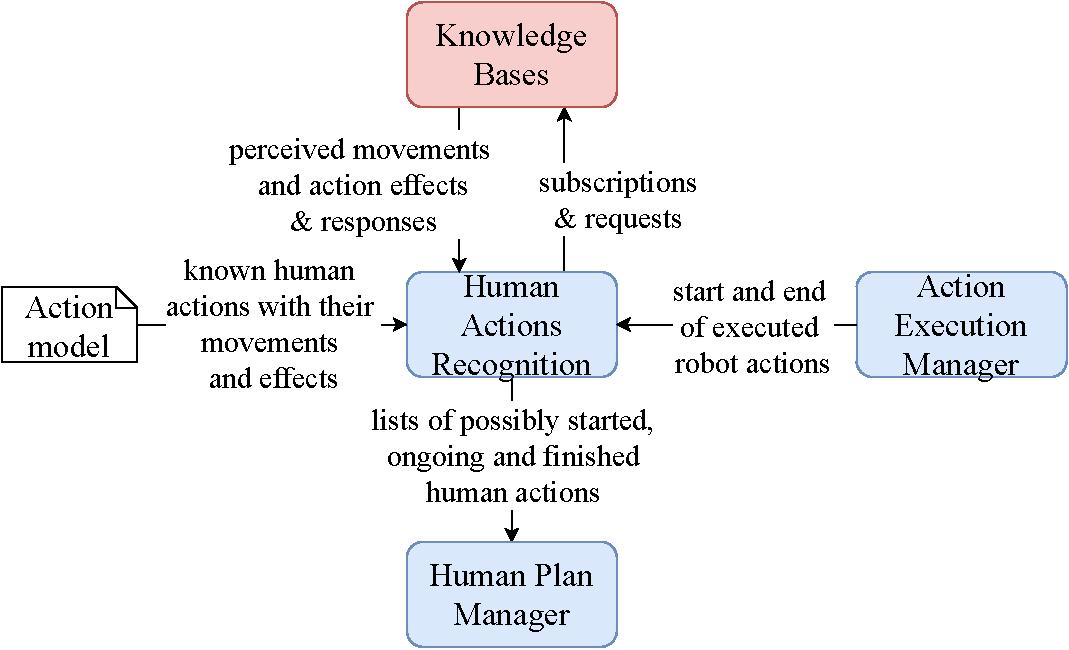
\includegraphics[width=0.8\linewidth]{figures/chapter2/action_reco_zoom.pdf}
	\caption{The \acrlong{ham} and the \acrshort{rja}s (in blue) and the component of the robotic architecture (in red) with which it interacts. It is fed by a file (in white) with description of the human actions the robot should recognize.}
	\label{chap6:fig:action_monitoring_zoom}
\end{figure}

In order to coordinate properly, humans monitor each other's when they are in a joint action (see Section~\ref{chap1:subsubsec:monitoring}). The robot needs the same kind of process to be able to assess if the human is doing the action of the plan it expects or not. This allows to follow the plan progress and to estimate the level of human engagement. Existing solutions exist to recognize human actions but none of them matched all our criteria which are: 
\begin{bulletList}
	\item it should be easy and quick to add a new action that the robot can recognize
	\item the process should output the action parameters
	\item the process should give information about the action progress, \ie modeling the action start and progression when possible and not only the end
	\item it needs to be robust to a potentially unreliable perception
	\item an available open-source code 
\end{bulletList}

Thus, we implemented our own model-based solution with an \acrshort{rja} dedicated to \acrfull{ham}. Figure~\ref{chap6:fig:action_monitoring_zoom} shows its relations with the other \acrshort{rja} of \acrshort{jahrvis}  and components of the robotic architectures. It could be replaced later with a more complex solution meeting the needs, but even though the current one is quite simple, it has interesting properties, matching the criteria presented above.

The \acrshort{ham} relies on the action model presented in Section~\ref{chap6:par:act_rep} which it loads at initiation. We chose to base our action recognition process on human movements and action effects that the robot can observe. As it needs to recognize them, it extracts the predicate types corresponding to those and subscribes to updates about these facts to Ontologenius as explained in Section~\ref{chap6:sec:know}. 

Continuously, the \acrshort{ham} \acrshort{rja} receives facts and human movements that are present in the action model, and sends to the \acrfull{hpm} \acrshort{rja} three types of data about human actions: 
\begin{bulletList}
	\item list of actions that may have started that we coined \emph{possibly started actions}
	\item list of actions that may be progressing that we coined \emph{possibly progressing actions}
	\item list of actions that are estimated as finished that we coined \emph{possibly achieved actions} 
\end{bulletList}

\begin{figure}[!hbt]
	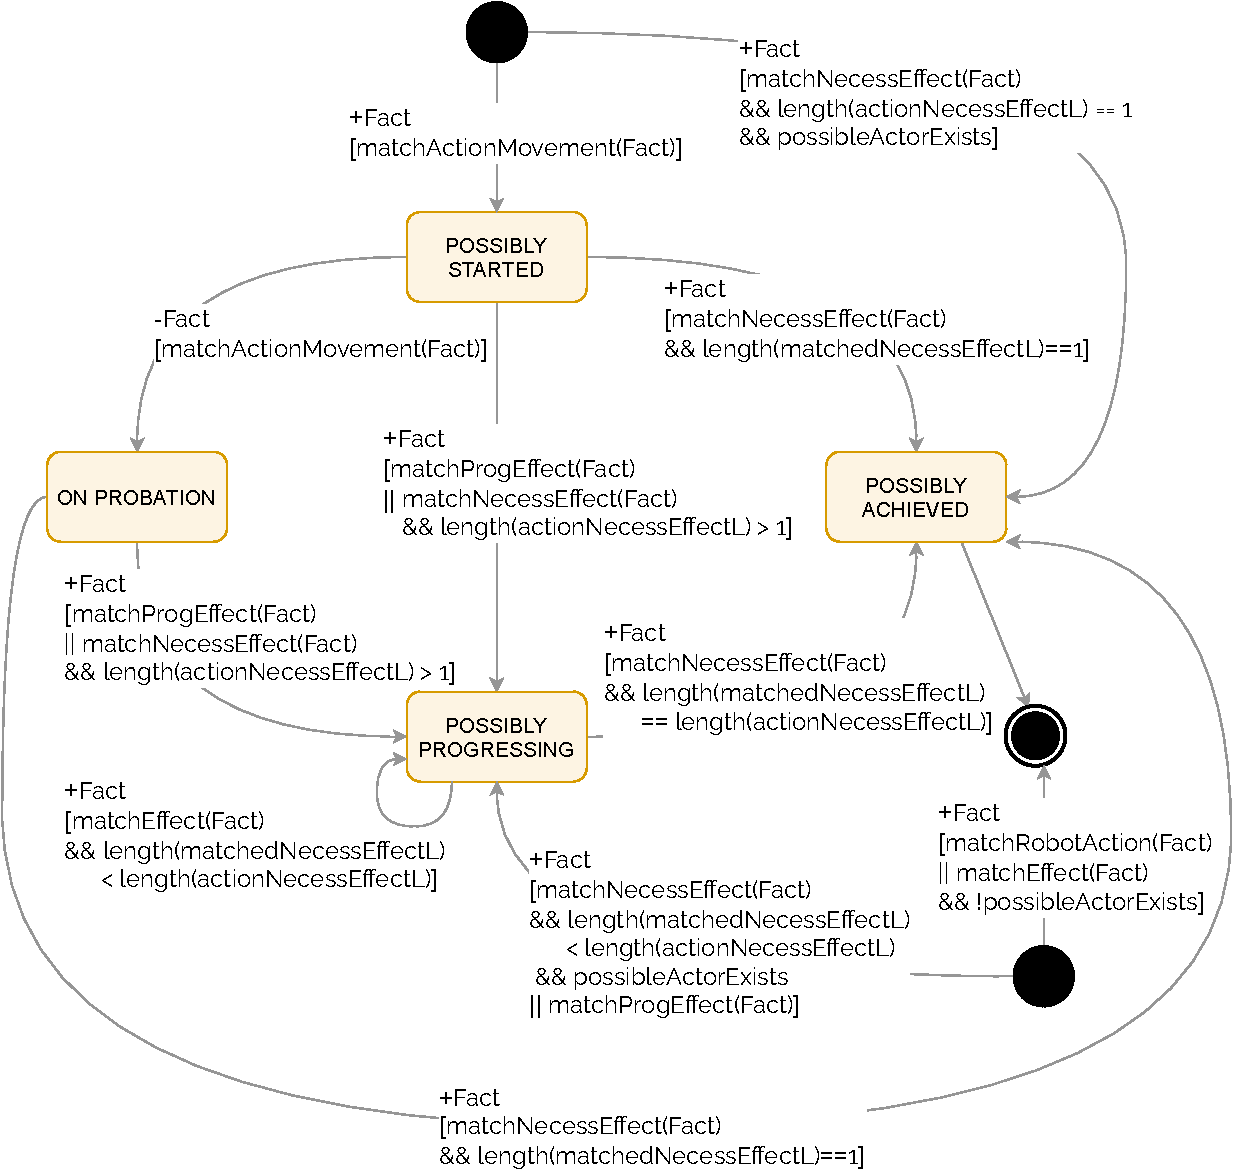
\includegraphics[width=\linewidth]{figures/chapter2/action_sm.pdf}
	\caption{Representation of the \acrfull{ham} \acrshort{rja} in the form of a Finite State Machine representing the state of one action. Transitions are composed of a triggering event (+Fact or -Fact) and a condition between square brackets. Variable names ending with a ``L'' are list of effects, either the necessary effect list of a given action in the model (actionNecessEffectL) or the list of facts in the current worldstate corresponding to the effects of a given action (matchedNecessEffectL).}
	\label{chap6:fig:action_monitoring}
\end{figure}

Action states are updated according to the facts defined in the human action model that the \acrshort{ham} receives. When the state of an action changes to \emph{possibly started}, \emph{possibly progressing} or \emph{possibly achieved}, the affected list is updated and sent to the \acrshort{hpm}. 

We chose to use the term \emph{possibly} to describe these states as the system is aware that some estimations of action states do not correspond to what is happening in the real world (\eg each time the human moves their hand, it can trigger a possibly started action), but they allow the system to have an idea of what might be going on.

The algorithm we developed can be depicted in the form of a Finite State Machine representing the state of one action as shown in Figure~\ref{chap6:fig:action_monitoring} and is implemented in ASL. Many State Machines can run simultaneously, one for each action that is estimated to be in one of the states. The parameters field of an action are filled as it is making progress through the states, according to the movement and effects allocated to this action.


\thispagestyle{example}

Each transition is triggered by the addition or the deletion of a fact. Using Jason rules\footnote{They are quite similar to Prolog rules.}, facts are analyzed to see if they match a movement or an effect of a known action. For example, if we look at the Place action example presented in Section~\ref{chap6:par:act_rep}, when performed by a human, it expects the fact \fact{handMovingToward}{Human}{Support} as a movement. Therefore, receiving \fact{rightHandMovingToward}{human\_0}{placement\_1} will match a Place action movement and will add the action to the list of \emph{possibly started actions}. However, receiving \fact{rightHandMovingToward}{human\_0}{phone} will not, as the phone does not belong to the Support class (but this fact may be useful for recognizing another action).
 
It is not shown on the Figure for clarity reasons, but each state, except \emph{possibly achieved}, has a transition to the final state which is triggered by a time deadline. Currently, this timeout is the same for each action but as every action type might be of different lasting, a deadline could be specifically set for each one. All the other transitions of the state machine are described in Table~\ref{chap6:tab:action_monitoring}.


\newgeometry{left=1in,right=1in,top=1in,bottom=0.5in,includefoot,includehead,headheight=13.6pt}

\begin{landscape}
%	\vspace*{\fill}
	\begin{table}[htb!]
	\caption{Description of the Finite State Machine shown in Figure~\ref{chap6:fig:action_monitoring}. Inputs are triggering events (+Fact or -Fact) and conditions are between square brackets. Variable names ending with a ``L'' are list of effects, either the necessary effect list of a given action in the model (actionNecessEffectL) or the list of facts in the current worldstate corresponding to the effects of a given action (matchedNecessEffectL).}
	\label{chap6:tab:action_monitoring}
	\begin{tabularx}{\linewidth}{| c | c | c | X |}
		Current State & Input and Condition & Next State & Explanation\\ 
		\hline \hline
	\multirow{4}{*}{Initial State}  & +Fact [matchActionMovement(Fact)] & Possibly Started & When a fact matching a movement and filling the preconditions for a given action is received, \acrshort{ham} computes that the human may have initiated an action. \\  
		\cline{2-4}
		&  \makecell{+Fact [matchNecessEffect(Fact) 
			\\ \&\& length(actionNecessEffectL)	== 1
			\\ \&\& possibleActorExists]} & Possibly Achieved & The robot may have missed the movement or the progression effect of an action because it was not looking or the perception did not detect it. Then when a necessary effect is received and that only one exists for the action, the action is estimated as achieved if it is possible to find an agent who may have performed it. For now, the finding function is looking for humans in the vicinity of the effect objects, and if there are several humans, it selects the closest one.\\  
		\cline{2-4}
		&  \makecell{+Fact [matchNecessEffect(Fact) 
		\\ \&\& length(matchedNecessEffectL)
		\\ < length(actionNecessEffectL)
		\\ \&\& possibleActorExists
		\\ || matchProgEffect(Fact)]} & Possibly Progressing & Similarly to the case above, the robot may have missed the movement or the progression effect of an action. However, if this action has several necessary effects, the action is considered as progressing.\\  
		\cline{2-4}
		& \makecell{+Fact [matchRobotAction(Fact)
		\\ || matchEffect(Fact) \&\& !possibleActorExists]} & Final State & The \acrshort{ham} is aware of the actions executing by the robot so it does not mismatch its action effects with the ones of another agent. If an effect matches, nothing happens. Likewise, if an effect is detected but no agent could be found that might have done it.\\  
		\hline 
	\end{tabularx}
\end{table}
\vspace*{\fill}
 \begin{table}[htb!]
 	\caption*{Table~\ref{chap6:tab:action_monitoring}: (continued)}
	\begin{tabularx}{\linewidth}{| c | c | c | X |}
		Current State & Input and Condition & Next State & Explanation\\ 
		\hline \hline
		\multirow{3}{*}{Possibly Started}  
		& \makecell{+Fact [matchProgEffect(Fact)
			\\ || matchNecessEffect(Fact) 
			\\ \&\& length(actionNecessEffectL) > 1]} & Possibly Progressing & When a fact corresponding to a progression effect of the started action is received, or it matches a necessary effect but there are more than one for this action, \acrshort{ham} reinforces its estimation that this action is ongoing by setting it to the progressing state.\\  
		\cline{2-4}
		& \makecell{+Fact [matchNecessEffect(Fact) 
			\\ \&\& length(matchedNecessEffectL) == 1]} & Possibly Achieved 
		& When a fact corresponding to a necessary effect is received and that there is only one for the started action, the action is considered as achieved as the robot is able to observe its effect and that it had observed the human starting it.\\  
		\cline{2-4}
		& -Fact	[matchActionMovement(Fact)] & On Probation & When a movement fact is removed from the belief base without having observed an effect, it might mean that it was a human hesitation or a false estimation and that the action is not starting. However, it might also be the robot perception being sporadic and so the action goes in this temporary state waiting for a potential coming effect.\\  
		\hline
	\end{tabularx}
\end{table}
\vspace*{\fill}
  \begin{table}[htb!]
  	\caption*{Table~\ref{chap6:tab:action_monitoring}: (continued)}
	\begin{tabularx}{\linewidth}{| c | c | c | X |}
		Current State & Input and Condition & Next State & Explanation\\ 
		\hline \hline
		\multirow{2}{*}{On Probation} 
		& \makecell{+Fact [matchProgEffect(Fact)
			\\ || matchNecessEffect(Fact)
			\\ \&\& length(actionNecessEffectL) > 1]} & Possibly Progressing & An effect is detected and the action state is resumed.\\
		\cline{2-4}
		& \makecell{+Fact [matchNecessEffect(Fact) 
			\\ \&\& length(matchedNecessEffectL) == 1]} & Possibly Achieved 
		& A necessary effect is detected and as there is only one for this action, it is considered as achieved.\\
		\hline
		\multirow{2}{*}{Possibly Progressing} 
		& \makecell{+Fact [matchNecessEffect(Fact) 
			\\ \&\& length(matchedNecessEffectL)
			\\ == length(actionNecessEffectL)]} & Possibly Achieved 
		& A necessary effect is received and in total, for this action, there was as many necessary effects received as the ones defined for this action.\\
		\cline{2-4}
		& \makecell{+Fact [matchEffect(Fact) 
			\\ \&\& length(matchedNecessEffectL)
			\\ < length(actionNecessEffectL)]} & Possibly Progressing 
		& When an action effect is received and that either it is another progressing or not the last necessary effect expected for the action, the action state remains progressing.\\  
		\hline
		Possibly Achieved & -- & Final State & When an action is estimated as achieved, this is its final state.\\
		\hline
	\end{tabularx}
	
\end{table}
\vspace*{\fill}
\end{landscape}

\restoregeometry

When the software starts, the \acrshort{ham} extracts from the internal action representation presented in Section~\ref{chap6:subsec:action_rep}, all the types of facts that should be monitored. Then, it queries Ontologenius to send it each update about these facts. Thus, when the robot designers decide that a new action should be recognized by the robot, the only thing to add is the action model in \acrshort{jahrvis} belief base.

Moreover, sometimes new facts are actually effects of robot actions. In order to avoid that robot actions are mistaken for human ones, the \acrshort{aem} signals to the \acrlong{ham} when the robot executes a given action of the plan. 

Finally, all the functions to check if a new fact update matches an action effect are Jason rules. They rely on the external knowledge base, here Ontologenius, as there is a need to compare the predicate object and subject expected classes of an action effect with the received ones.

\thispagestyle{example}
\subsection*{Examples}
Now, we give an insight of what happens in the system when the human performs pick and place actions, based on the StackBuildingTask example. We will present several cases in pictures and one completed with a timeline and a sequence diagram.

\begin{figure}[!htp]
	\subfloat[The human has his hand moving toward the blue cube and the stick (the longer blue cube ).]{\label{chap6:fig:action_monitoring_photos_toward}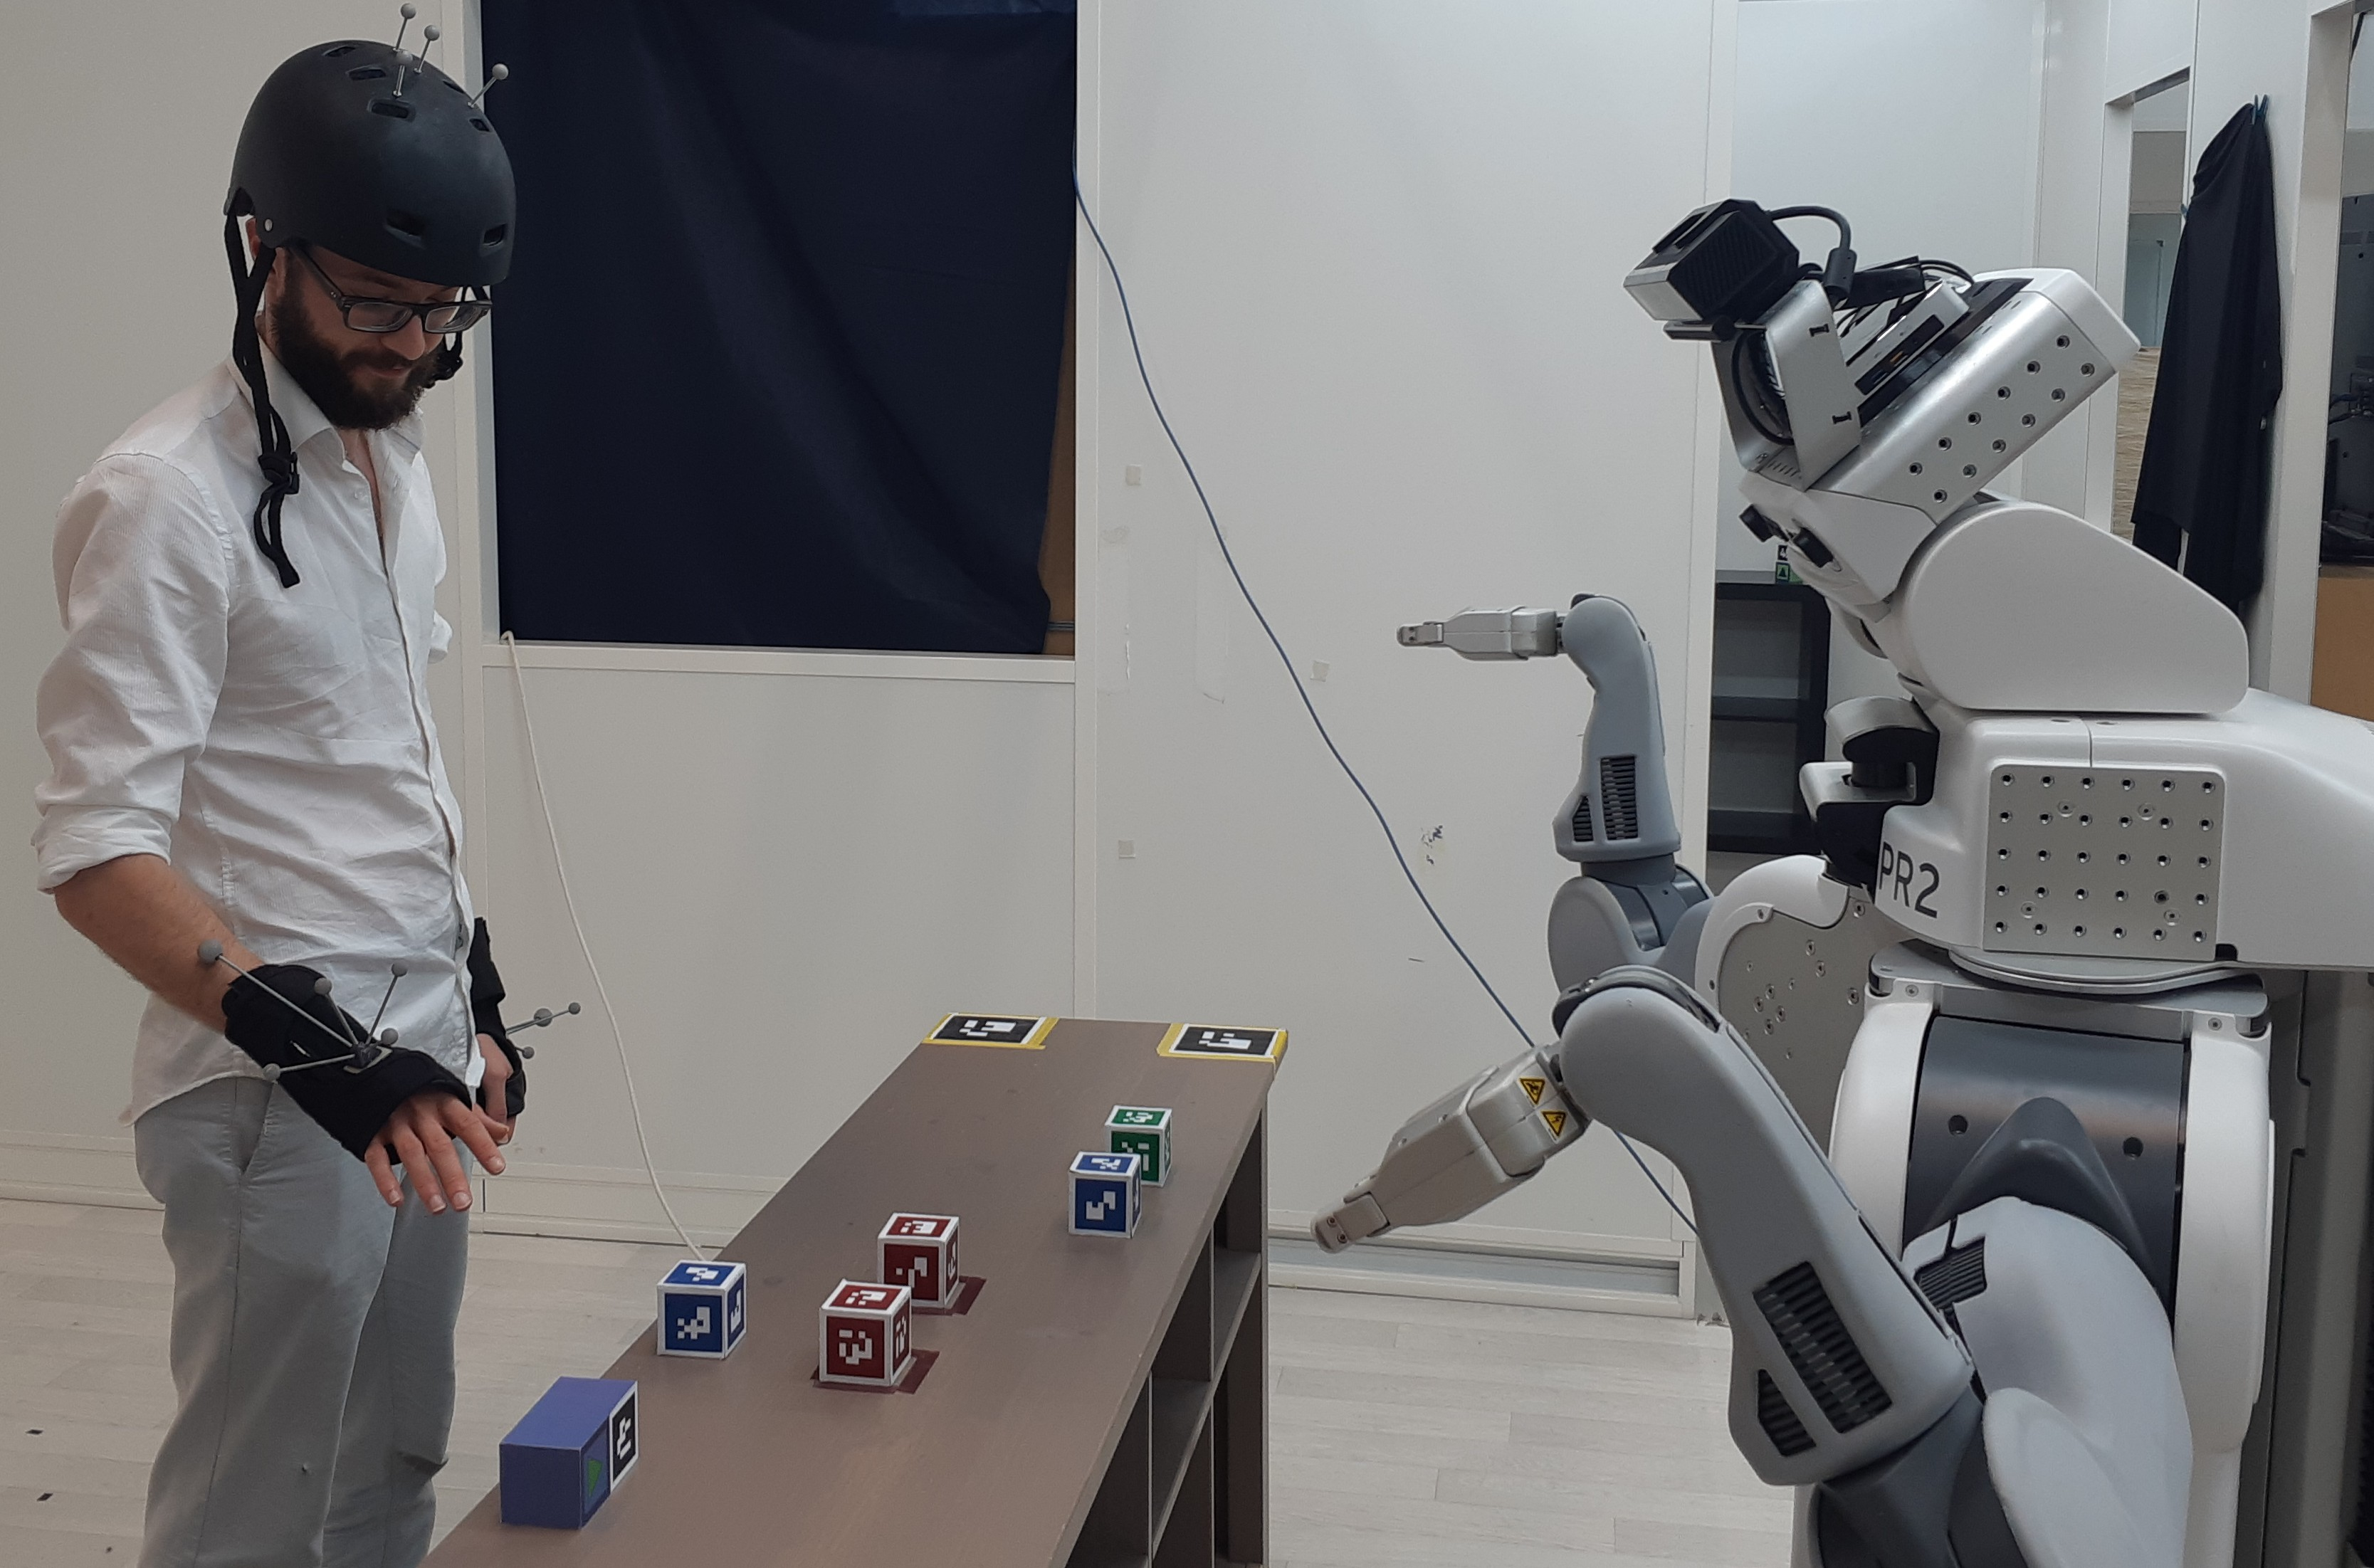
\includegraphics[width=0.3\linewidth]{figures/chapter2/moving_toward.jpg}}\hfill
	\subfloat[The human is holding the stick.]{\label{chap6:fig:action_monitoring_photos_holding}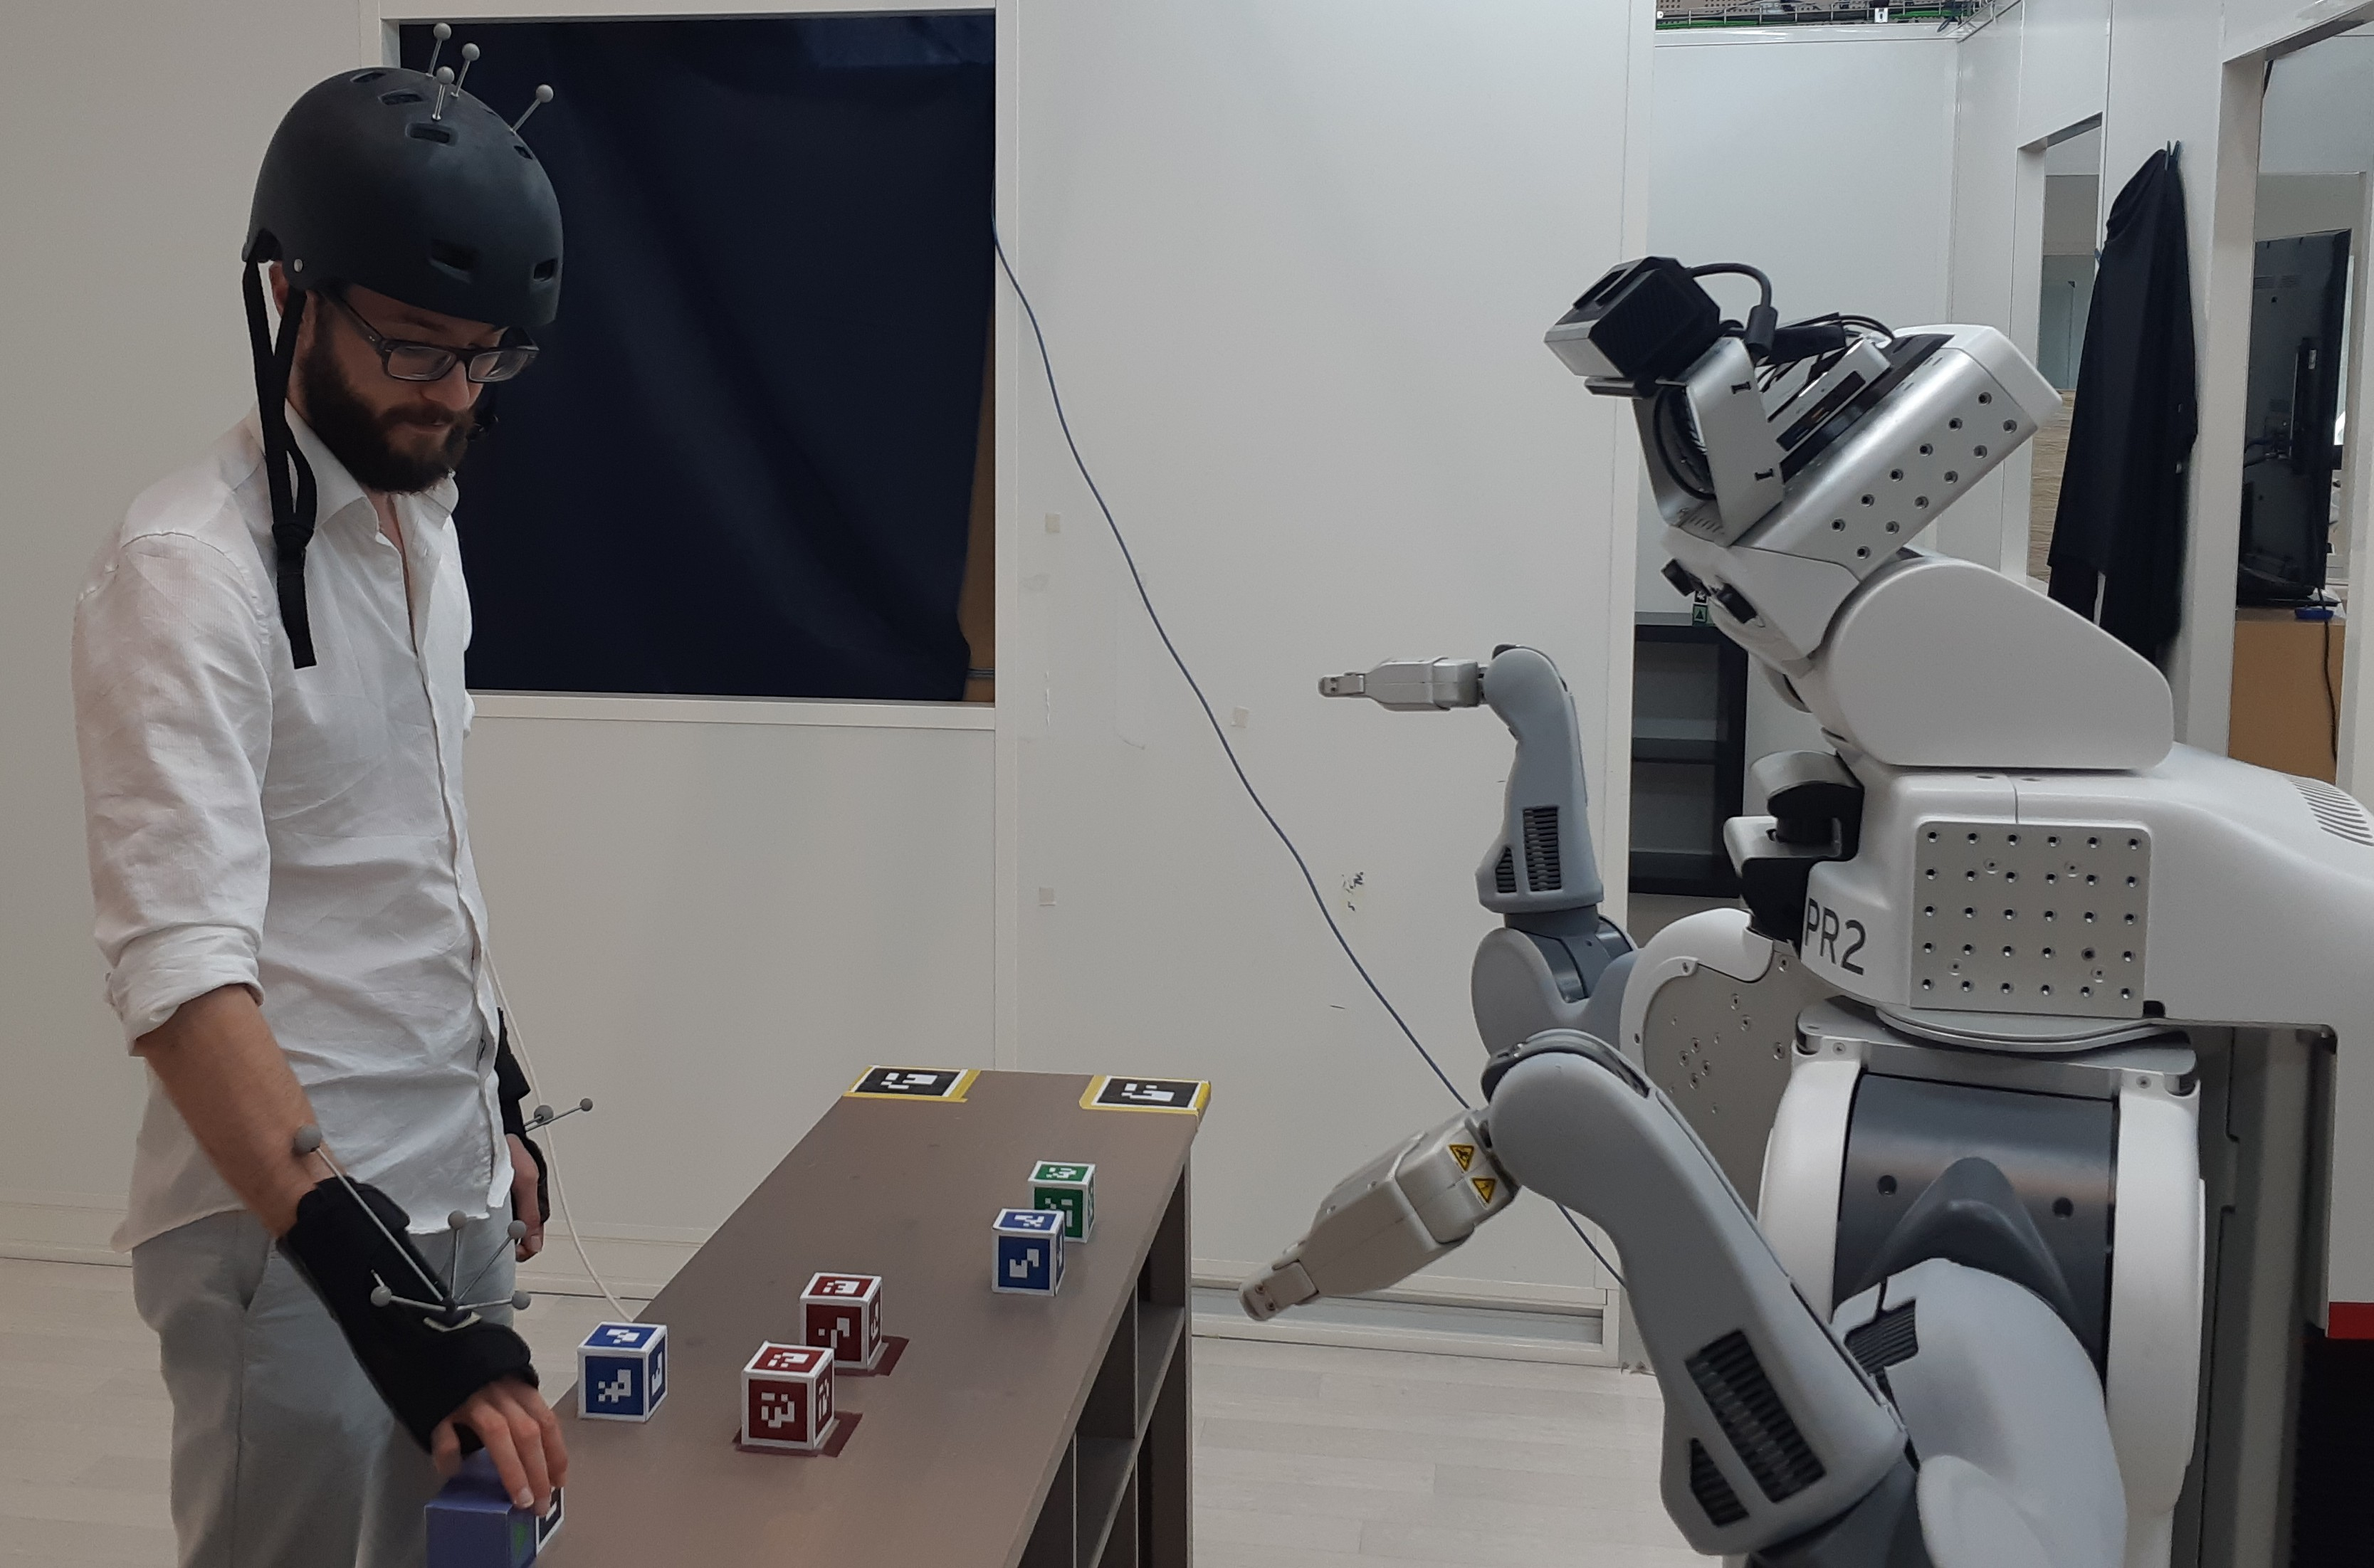
\includegraphics[width=0.3\linewidth]{figures/chapter2/holding_stick.jpg}}\hfill
	\subfloat[The human picked the stick, it is not of top of the table anymore.]{\label{chap6:fig:action_monitoring_photos_not_top}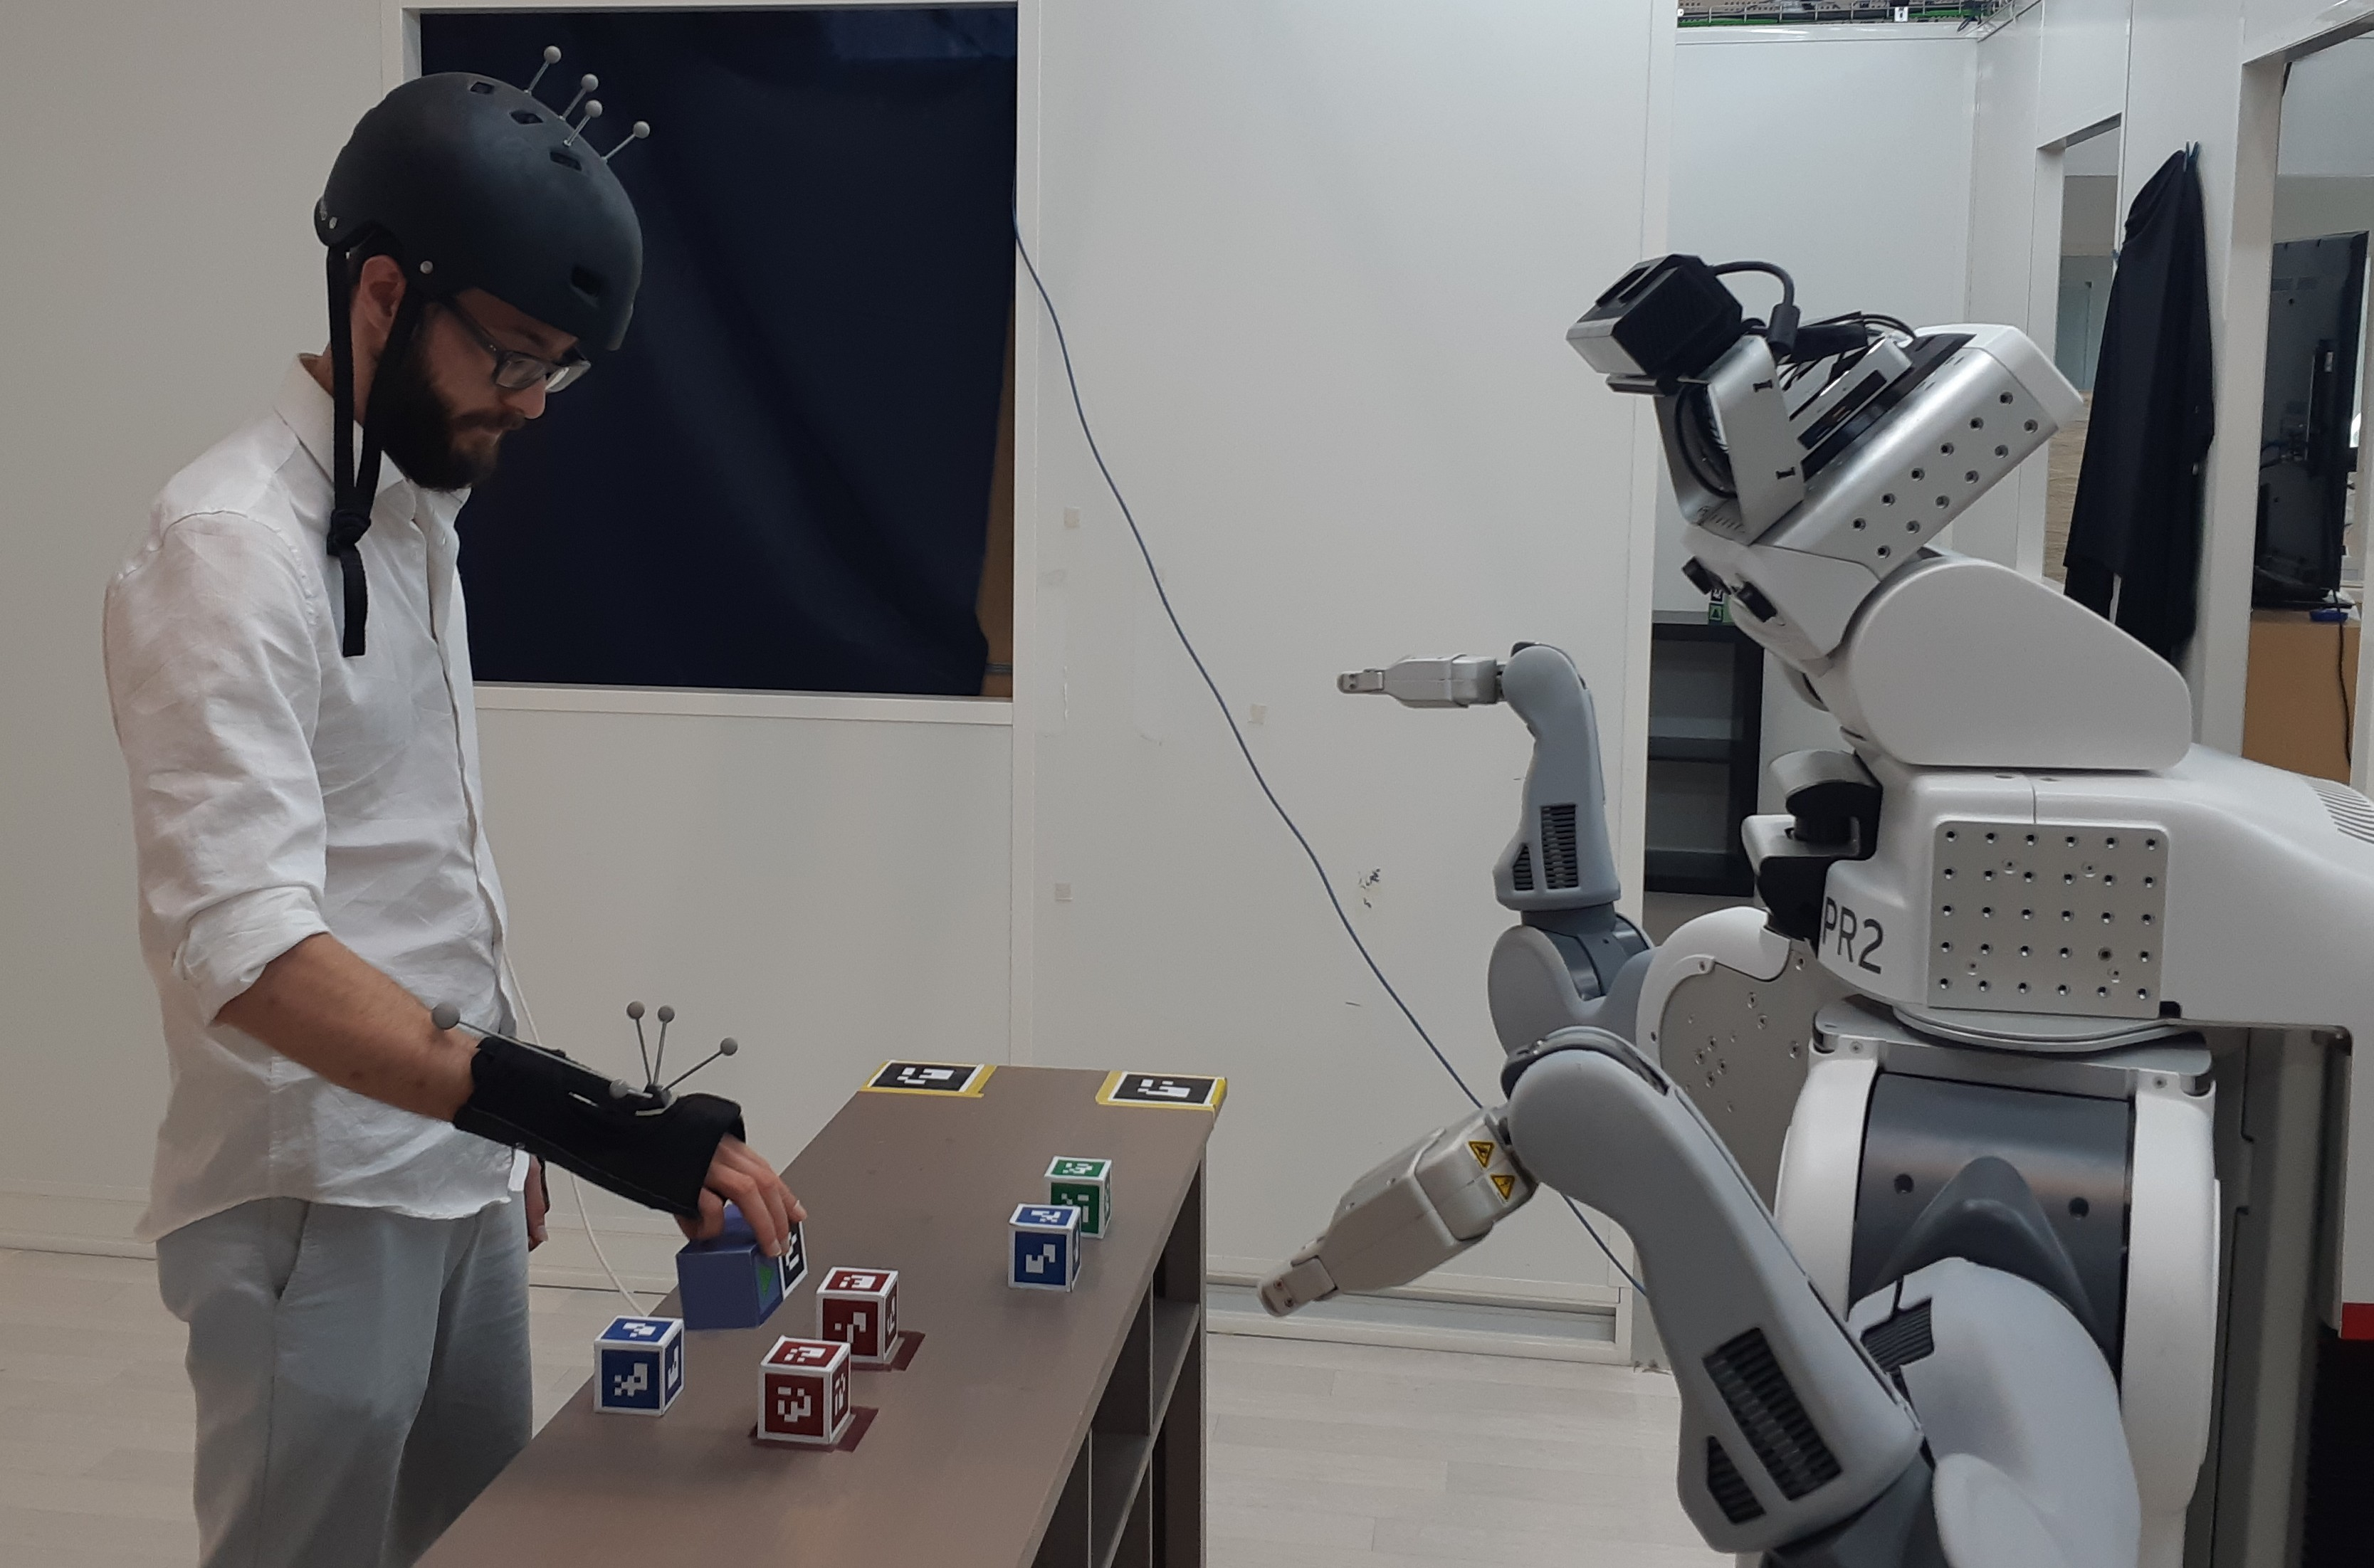
\includegraphics[width=0.3\linewidth]{figures/chapter2/not_top_stick.jpg}}\hfill
	\caption{Decomposition of a pick action of the stick.}
	\label{chap6:fig:action_monitoring_photos_pick}
\end{figure}

\paragraph{The human has to pick the stick}

The scene is depicted in Figure~\ref{chap6:fig:action_monitoring_photos_pick}. There are two cubes on the human side: the stick and the blue cube. Both red cubes are on their placements so this is the moment where the human should pick the stick. Figure~\ref{chap6:fig:action_reco_ex1_timeline} is a timeline showing on the right the facts arrived from the situation assessment, fed to the \acrshort{kb}, and then sent to the \acrshort{ham}. First, the human starts to move his hand towards the table and the cubes (Figure~\ref{chap6:fig:action_monitoring_photos_toward}). No fact is received by the \acrshort{ham} about the table as it has subscribed to \fact{handMovingToward}{Human}{Pickable} and the table is not a Pickable. We can notice that the received facts are with the predicate \textit{rightHandMovingToward} which is a subproperty of \textit{handMovingToward}. Thus, as we can see in Figure~\ref{chap6:fig:action_reco_ex1}, it triggers the possible start of two pick actions, one for the stick and the other one for the blue cube. Then, the human has the stick in his hand but it is still on the table (Figure~\ref{chap6:fig:action_monitoring_photos_holding}), thus the pick action with the stick is considered as possibly progressing and the pick action with the blue cube remains as possibly started. Finally, the human withdraws his hand, holding the stick and so the stick is not on the table anymore (Figure~\ref{chap6:fig:action_monitoring_photos_not_top}). Therefore, the action is estimated as possibly achieved. As it was the one expected to be the next action to perform, the \acrlong{hpm} left aside the started action with the blue cube and selected the one with the stick as the one that was ongoing. It fed Ontologenius with the action and its associated parameters and Mementar with the start and end times as we can see in Figure~\ref{chap6:fig:action_reco_ex1_timeline}.

\paragraph{The human picks the blue cube while the robot is not looking} 

The scene is depicted in Figure~\ref{chap6:fig:action_monitoring_photos_missing}. The robot is not looking as it is picking the green cube as shown in Figure~\ref{chap6:fig:action_monitoring_photos_not_looking}. Then, as it places its cube on the stack (Figure~\ref{chap6:fig:action_monitoring_photos_now_looking}), it looks in the direction of the blue cube former position. Thus, the Situation Assessment produces the deletion of the fact \fact{isOnTopOf}{blue\_cube\_2}{table\_1} which is signaled to the \acrshort{kb}s which information is sent to the \acrshort{ham}. Then, the \acrshort{ham} evaluates if a human agent could be at the origin of this change in the environment, associated to a pick action according to the human action model. And, the answer is yes and a pick action of the blue cube is allocated to the present human.
\thispagestyle{example}
\begin{figure}[!hbtp]
	\subfloat[The human is picking the blue cube while the robot is not looking as it is picking the green cube. Consequently, the robot does not know that the human performed an action. ]{\label{chap6:fig:action_monitoring_photos_not_looking}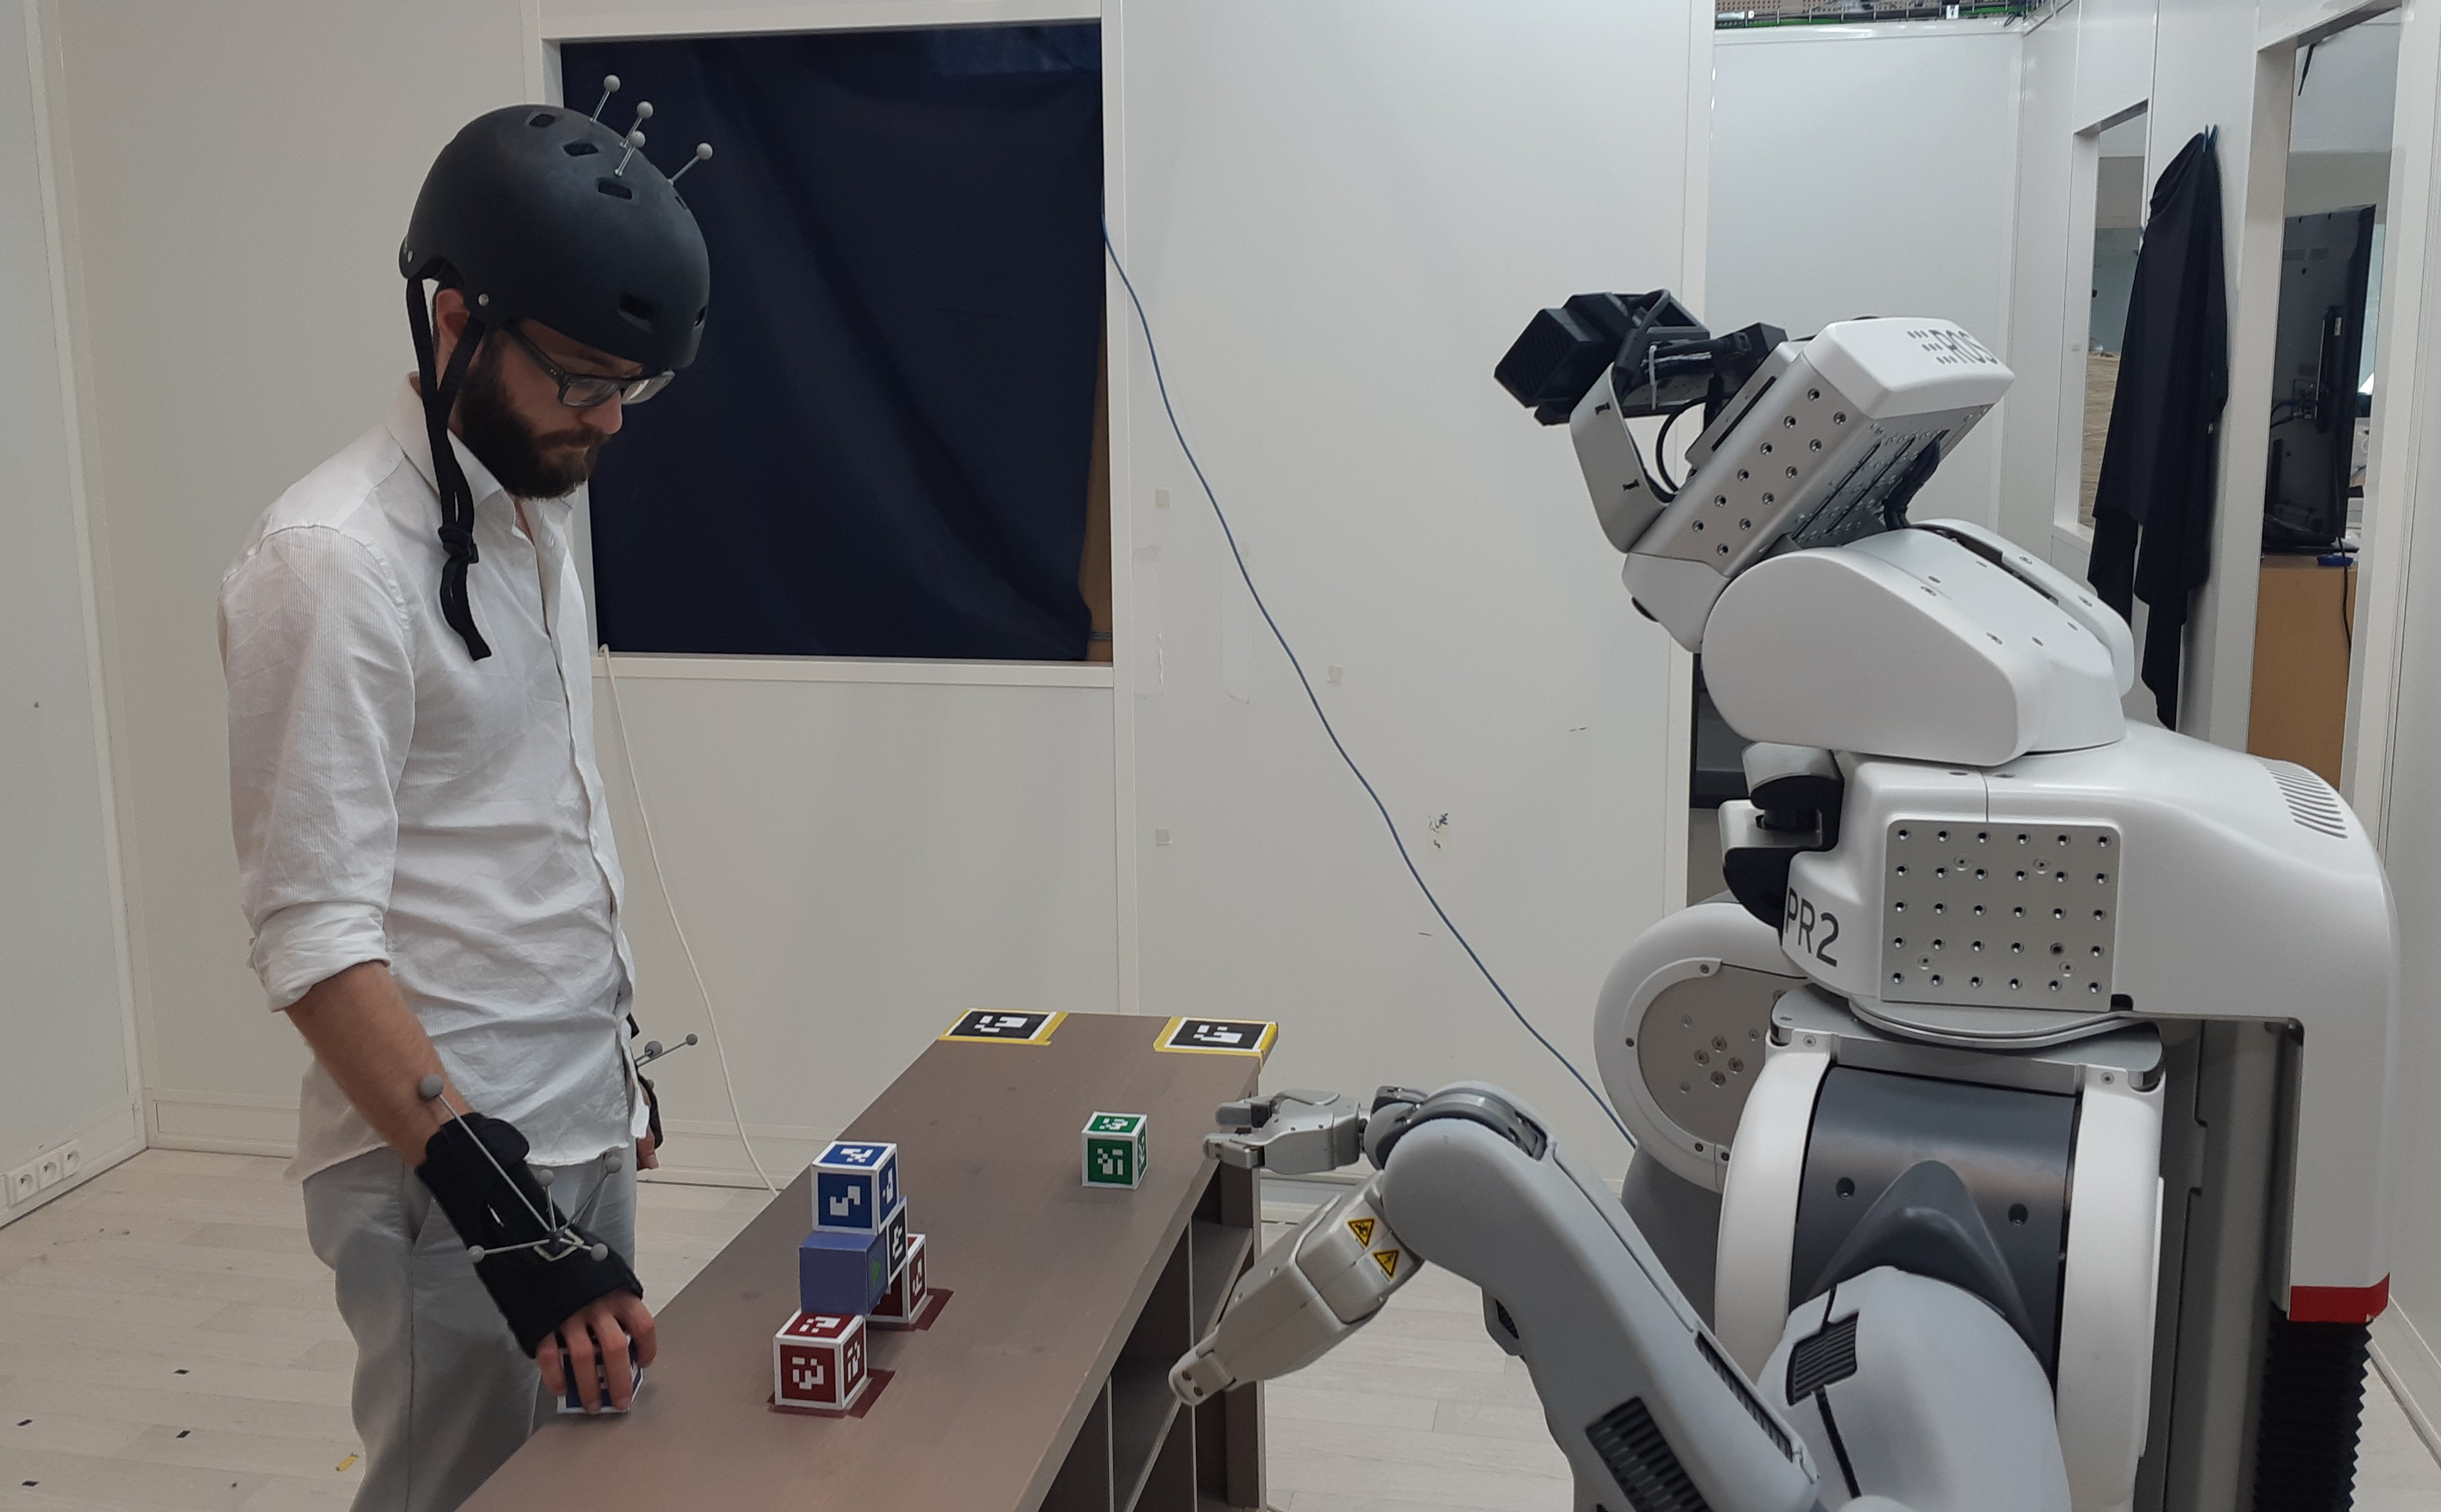
\includegraphics[width=0.45\linewidth]{figures/chapter2/looking_somewhere_else.jpg}}\hfill
	\subfloat[The robot is looking again in the human direction and observes that the blue cube is not on the table anymore. It deduces that the human has taken it and so performed the action in the plan.]{\label{chap6:fig:action_monitoring_photos_now_looking}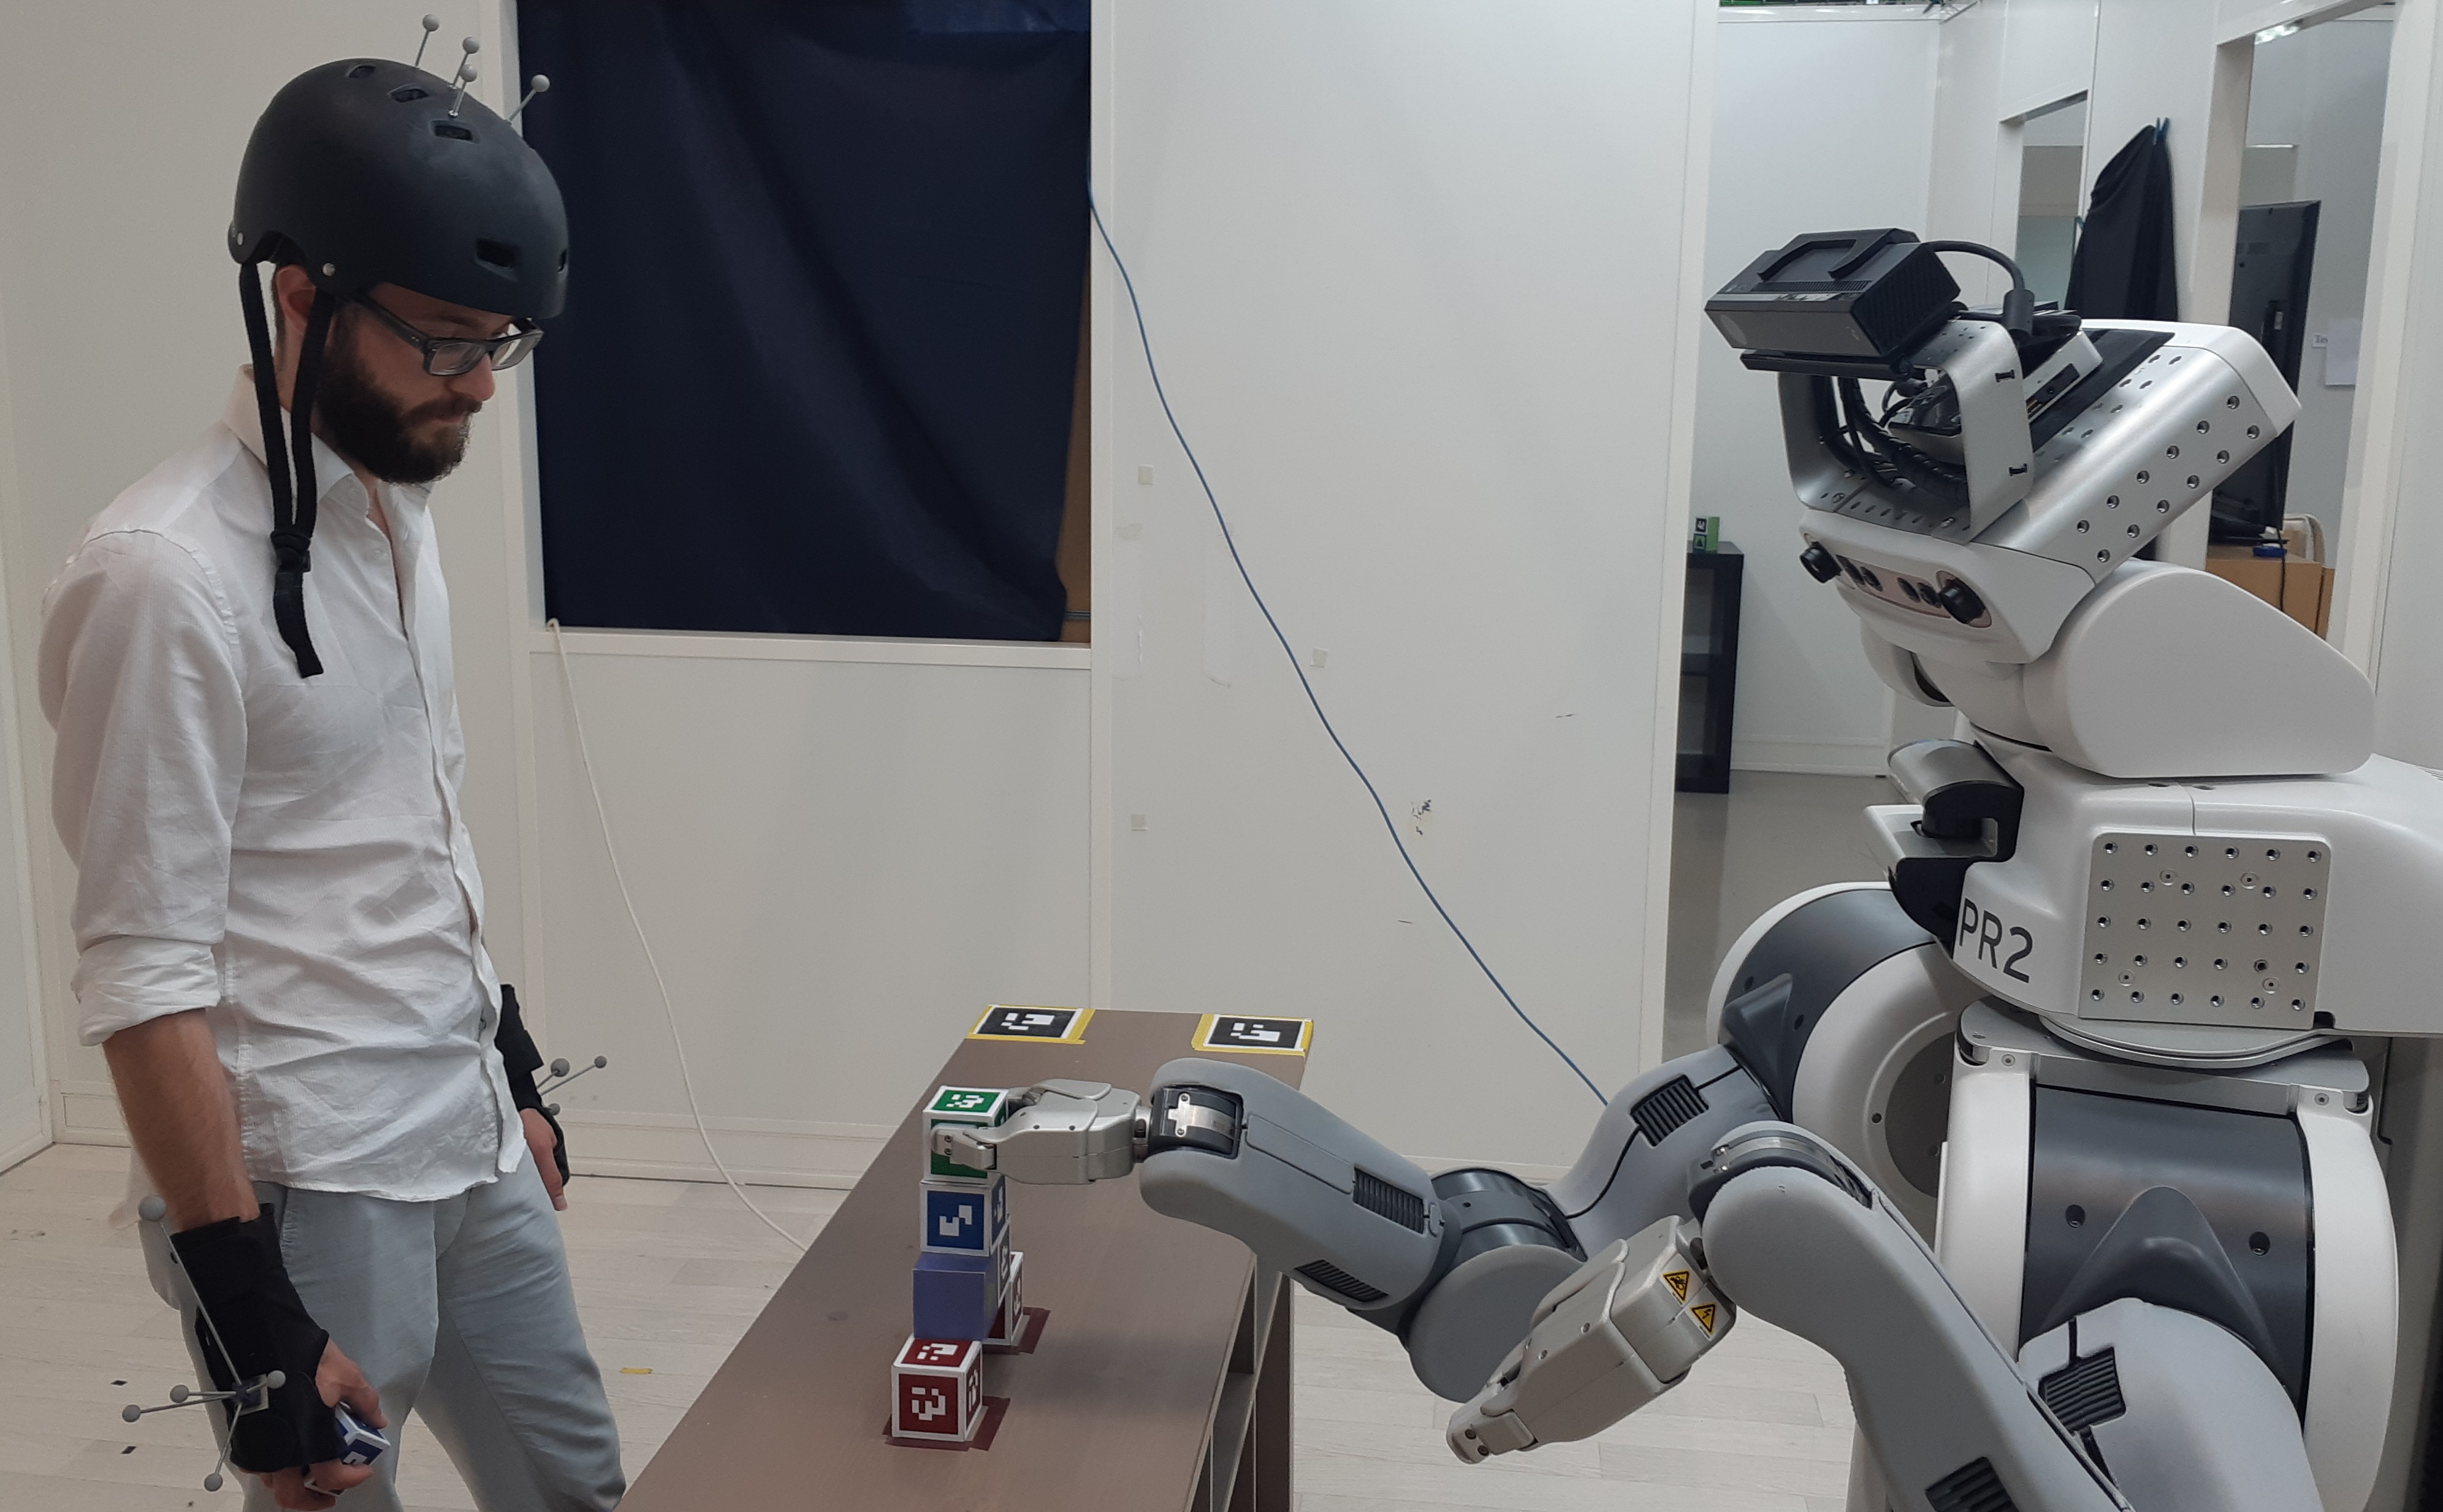
\includegraphics[width=0.45\linewidth]{figures/chapter2/now_looking.jpg}}\hfill
	\caption{The robot does not see the human picking the blue cube but then it deduces that he is the one to have performed the action.}
	\label{chap6:fig:action_monitoring_photos_missing}
\end{figure}
	
\newgeometry{left=0.9in,right=0.9in,top=1.1in,bottom=0.5in}
\begin{landscape}
	\begin{figure}[!htb]
		\centering
		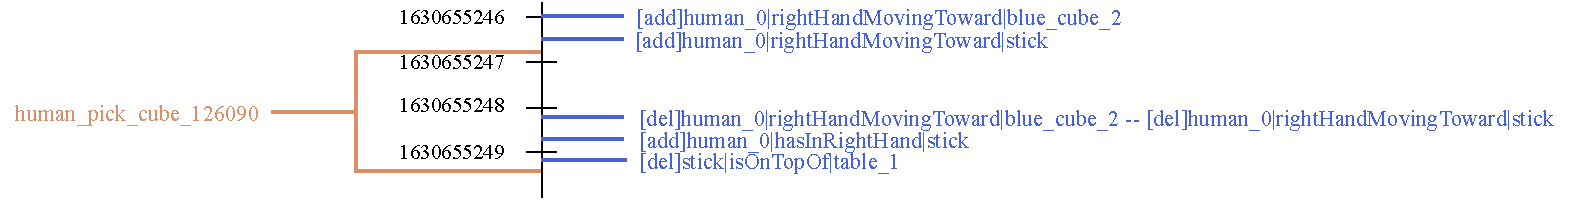
\includegraphics[width=0.9\linewidth]{figures/chapter2/action_reco_1.pdf}
		\caption{Timeline produced by Mementar on which appear facts from perception (blue, on the right) and the action added by the \acrlong{hpm} based on data from the \acrlong{ham} (orange, on the left). Numbers on the axis are time in milliseconds (epoch time).}
		\label{chap6:fig:action_reco_ex1_timeline}
	\end{figure}
	
	\begin{figure}[!htb]
		\centering
		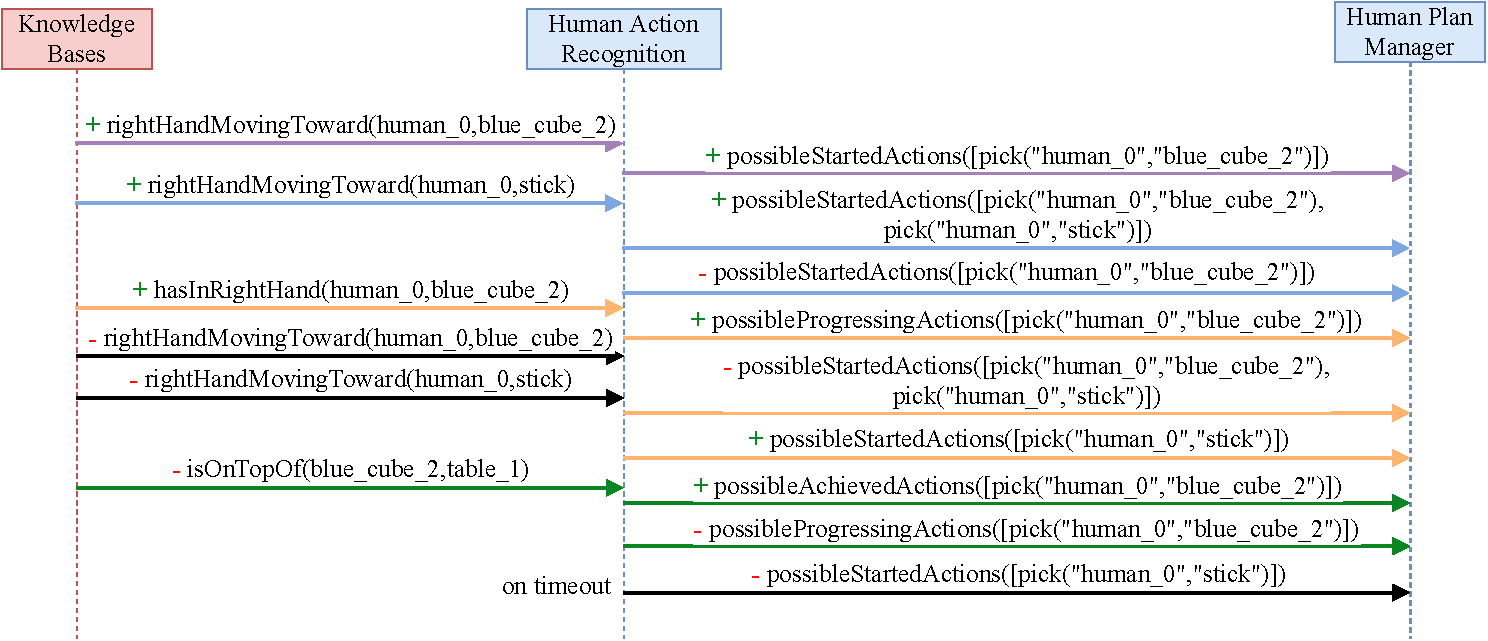
\includegraphics[width=0.75\linewidth]{figures/chapter2/action_monitoring_ex1.pdf}
		\caption{Sequence diagram for a pick action. The \acrshort{kb}s sends to the \acrshort{ham} the perceived facts to which the \acrshort{ham} subscribed. The \acrshort{ham} processes these facts through State Machines as presented above. Then it output action states which are sent to the \acrfull{hpm}. Arrows from the \acrshort{ham} to the \acrshort{hpm} of the same color (except black) than an arrow going from the \acrshort{kb}s to the \acrshort{ham} are triggered by it. A green plus sign means that it is a belief addition in the \acrshort{rja}, a red minus sign means that it is a belief deletion.}
		\label{chap6:fig:action_reco_ex1}
	\end{figure}
\end{landscape}
\restoregeometry

\section{Shared Plans Handling}\label{chap6:sec:plan_handling}
In order to correctly perform collaborative tasks with humans, the robot needs to know how to perform them. One way is to have a planner with a domain, computing a plan at execution time based on its current knowledge about the environment and interaction. Then, the robot must be endowed with a way to manage the execution of this ``recipe''. As we place ourselves in the context of joint action, plans manipulated by the robot are shared plans, as presented in Section~\ref{chap6:subsec:shared_p_rep} (to differentiate from the ASL plans presented in Section~\ref{chap4:subsec:jason} which code all the \acrshort{rja}). We make the assumption that the human knows how to create their own plan in order to reach the shared goal. So, we consider it is not necessary to verbalize it from the outset.

We claim that the robot ability to handle and execute shared plan is enhanced when endowed with \acrfull{tom} (see Sections~\ref{chap1:sec:tom} and~\ref{chap2:subsec:tom_hri}), as shown by \cite{devin_2016_implemented}. It allows the robot to be aware of false beliefs or belief divergences in the human's point of view. When such things happen, it can react appropriately, either by acting or communicating. We gave the robot such an ability\footnote{The robot has a first-order \acrshort{tom}, it estimates the human knowledge about the task but it does not compute what the human thinks of the robot knowledge about the task (second-order \acrshort{tom})}, \textit{via} two processes: the \acrfull{rpm} and the \acrfull{hpm} (see Figure~\ref{chap5:fig:sup_overview}). Therefore, the first one handles the robot's beliefs about the plan and the action execution while the second handles the estimation of the human's beliefs about the plan and the communication with the human. The \acrshort{rja}s implementing these processes are presented in Sections~\ref{chap6:subsec:robot_plan} and~\ref{chap6:subsec:human_plan}.

As we designed \acrshort{jahrvis} to be as generic as possible, it can manage different kinds of human-robot plans as input: 
\begin{bulletList}
	\item shared plans in which each action is allocated to an agent as well as action parameters are given objects,
	\item shared plans in which actions might not be allocated to an agent at planning time and parameters might refer to objects with a semantic query, and
	\item conditional plans which anticipate different possibilities for the human decision/action. 
\end{bulletList} 

To generate these plans, we worked with two planners, \acrshort{hatp} and \acrshort{hatpehda} presented in Section~\ref{chap3:subsubsec:task_planner}.

\paragraph{``Usual'' shared plans with HATP and HATP/EHDA} The first type of shared plans handled are what we could call ``usual'' shared plans. Each action is allocated to an agent as well as action parameters are given objects. Thus, in this kind of plan, no decision is left to \acrshort{jahrvis} about who should execute the action or with what object.

\paragraph{AgentX shared plans with HATP}
The second type of shared plans is an extension of the work of Devin about postponing some decisions from planning time to execution time about the actor of some actions and some parameters~\citep{devin_2017_decisions}. In work previous to Devin, all the actions of the computed plans were allocated and completely instantiated during plan elaboration. 

We re-implemented her idea of \emph{AgentX} in our plan managers (with some modifications, for example we do not replan once an action is allocated as we are able to identify in real-time if a next action is still feasible or not), enabling the \emph{choice} of the agent who should perform the action at execution time when the planner has computed that both agents could do it. This a mean to specify a goal in a more abstract way. Thus, when an action can indifferently be done by both agents, the planner returns  $\Pi=\langle id_\Pi,state_\Pi,name_\Pi,\text{AgentX},params_\Pi,preds_\Pi,\Delta_\Pi\rangle$. In this case, according to what \acrshort{jahrvis} estimates the human wants to do, it can allocate the action to itself or to them. Therefore, in the StackBuildingTask example, instead of having the planner arbitrary choosing which agent, the human or the robot, will place the first blue cube on the stick, it allocates it to AgentX.
\thispagestyle{example}

Then, a similar idea has also been developed by Devin for the parameters. Indeed, with usual \acrshort{hatp} plans, still with the StackBuildingTask example, the planner would have generated a plan where it is already decided that the robot should place, for example, its red cube on the placement 1 and the human should place theirs on the placement 2. We could have:
\begin{align*}
	\Pi_1=\langle id_{\Pi_1},\textsc{Planned},\text{human\_place\_cube},\text{human\_0}, [\text{red\_cube\_2,placement\_2}],&\\ preds_{\Pi_1},\Delta_{\Pi_1}\rangle&\\
	\Pi_2=\langle id_{\Pi_2},\textsc{Planned},\text{robot\_place\_cube},\text{pr2\_robot}, [\text{red\_cube\_1,placement\_1}],&\\ preds_{\Pi_2},\Delta_{\Pi_2}\rangle&
\end{align*}
  
However, actually, it does not matter here where which agent place their red cube. Thus, Devin introduced the use of the notion of object similarity: two \emph{similar} objects will have the same role in the task, they are functionally equivalent. With this new notion, instead of having the planner arbitrary deciding which individual should be used when two of them are equivalent, it manipulates object high-level names. Thus, in the StackBuildingTask, for the two first actions, we have:
\begin{align*}
\Pi_1=\langle id_{\Pi_1},\textsc{Planned},\text{human\_place\_cube},\text{human\_0}, [\text{red\_cube\_2,placement}],&\\ preds_{\Pi_1},\Delta_{\Pi_1}\rangle&\\
\Pi_2=\langle id_{\Pi_2},\textsc{Planned},\text{robot\_place\_cube},\text{pr2\_robot}, [\text{red\_cube\_1,placement}],&\\ preds_{\Pi_2},\Delta_{\Pi_2}\rangle&
\end{align*}

To have more expressiveness, we brought a new modification to the plans returned by \acrshort{hatp}, in collaboration with Guillaume Sarthou. Indeed, instead of returning an object generic name, it returns a \sparql{} query with the constraints used in the domain. Thus, keeping the same example as previously, the robot and human actions become:
\begin{align*}
\Pi_1=\langle & id_{\Pi_1},\textsc{Planned},\text{human\_place\_cube},\text{human\_0}, \\
&{}[\text{red\_cube\_2,?0 isA Placement NOT EXISTS \{ ?0 isUnder ?2. ?2 isA Cube \}}],\\ &preds_{\Pi_1},\Delta_{\Pi_1}\rangle\\
\Pi_2=\langle & id_{\Pi_2},\textsc{Planned},\text{robot\_place\_cube},\text{pr2\_robot}, \\
&{}[\text{red\_cube\_1,?0 isA Placement NOT EXISTS \{ ?0 isUnder ?2. ?2 isA Cube \}}],\\  &preds_{\Pi_2},\Delta_{\Pi_2}\rangle
\end{align*}
\thispagestyle{example}
This allows the \acrshort{rpm} to directly request Ontologenius to get an object list matching this query and to select an object among it at execution time. And, when the human performs an action with a \sparql{} query as parameter, the \acrshort{hpm} can check if the object on which the human is acting matches the query. We can see that this solution is enhanced compared to the one presented by Devin. Indeed, \verb'red_cube' does not tell that it should be reachable by an agent and that it should not be on the top of another cube yet but \verb'?0 isA Cube. ?0 hasColor red. ?0 isReachableBy ?1' \verb'NOT EXISTS { ?0 isOnTopOf ?2. ?2 isA Cube }' does. For example, in Devin, the reachability test was written in the plan manager of the supervisor, in a hard-coded manner. 

The plan for the StackBuildingTask example is presented in Figure~\ref{chap6:fig:plan_hatp}.

\begin{figure}[!htb]
	\centering
	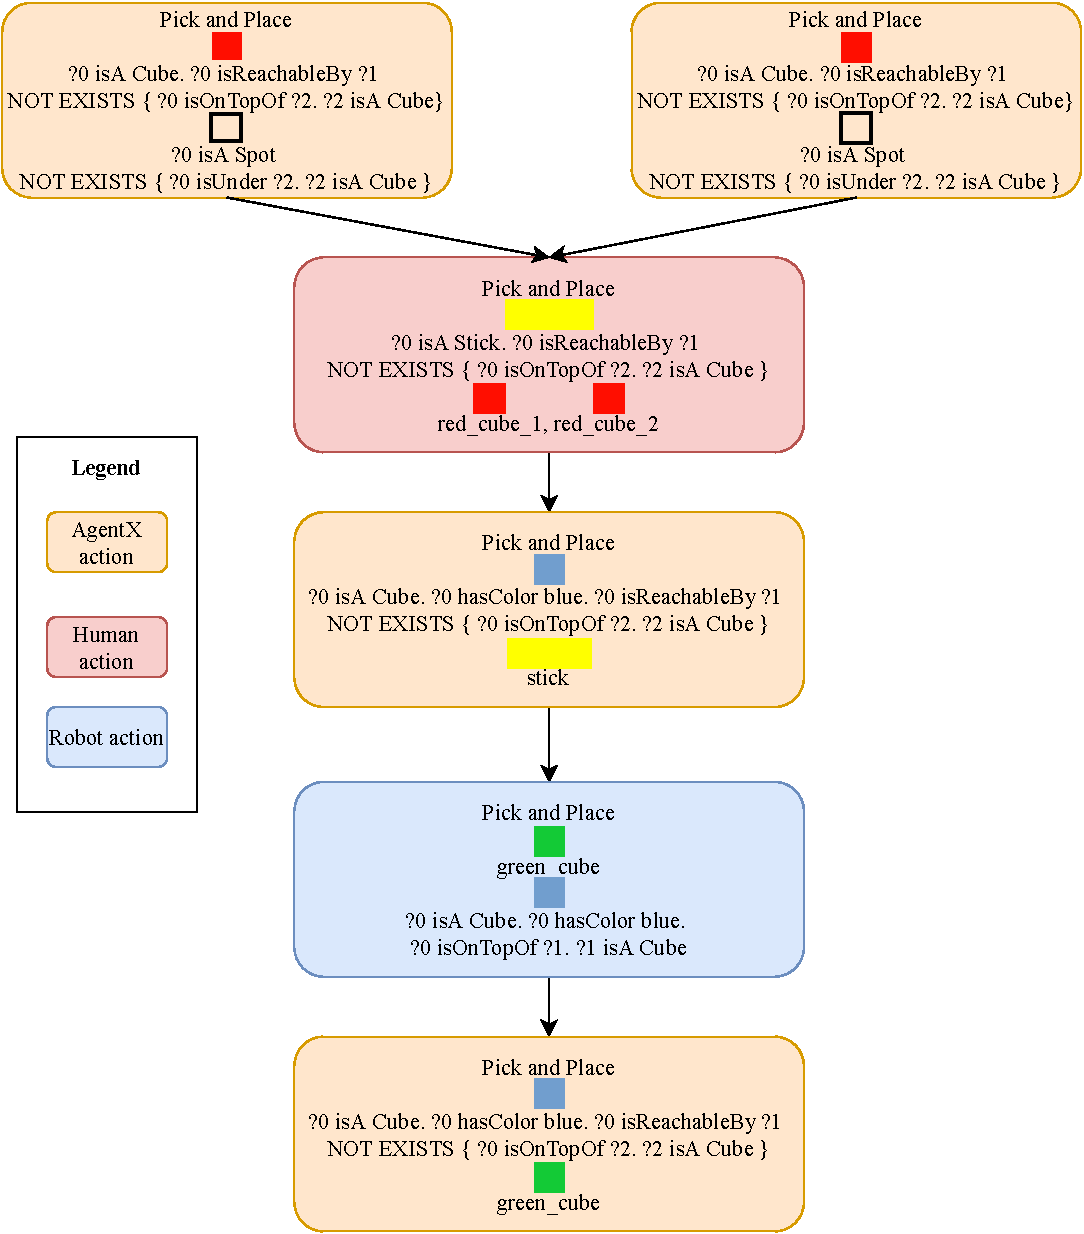
\includegraphics[width=\linewidth]{figures/chapter2/plan_hatp.pdf}
	\caption{A shared plan for the StackBuildingTask computed by \acrshort{hatp} with modifications to generate \sparql{} queries instead of object names as action parameters.}
	\label{chap6:fig:plan_hatp}
\end{figure}
\thispagestyle{example}
\paragraph{Conditional shared plans with HATP/EHDA}
Finally, the last type of shared plans we manipulated is conditional plan, generated by \acrfull{hatpehda}~\citep{buisan_2021_human}. It is another mean to postpone decision at execution time about an agent actor or parameters, with plans where branch junctions concern human decision. Moreover, it gives a better insight about the human's choices and decisions as they are formalized with the plan. For example, in Figure~\ref{chap6:fig:plan_building2}, is shown a conditional plan computed by \acrshort{hatpehda}\footnote{The domain for this plan was written by Guilhem Buisan} (we illustrate in Section~\ref{chap6:sec:example} how plans are handled by \acrshort{jahrvis} with an execution of the first actions of the plan). The plan is the one computed for the StackBuildingTask. Twice during the task, the human has a choice. First, they can choose where to place their red cube or to wait for the robot to choose for the placement. The second choice happens for the positioning of the first blue cube of the stack, either the human can place it on the stick or leave it to the robot. Thus, at planning time, the planner does not know the choice the human will make, but thanks to the conditional plan, all possible solutions are considered and it is up to \acrshort{jahrvis} to ``follow'' the proper branch depending on the human action detected during execution.

\todo{put on left and right pages}
\newgeometry{left=1in,right=1in,top=1.1in,bottom=0.5in}
\begin{landscape}
	\thispagestyle{example}
	\begin{figure}[!hp]
		\centering
		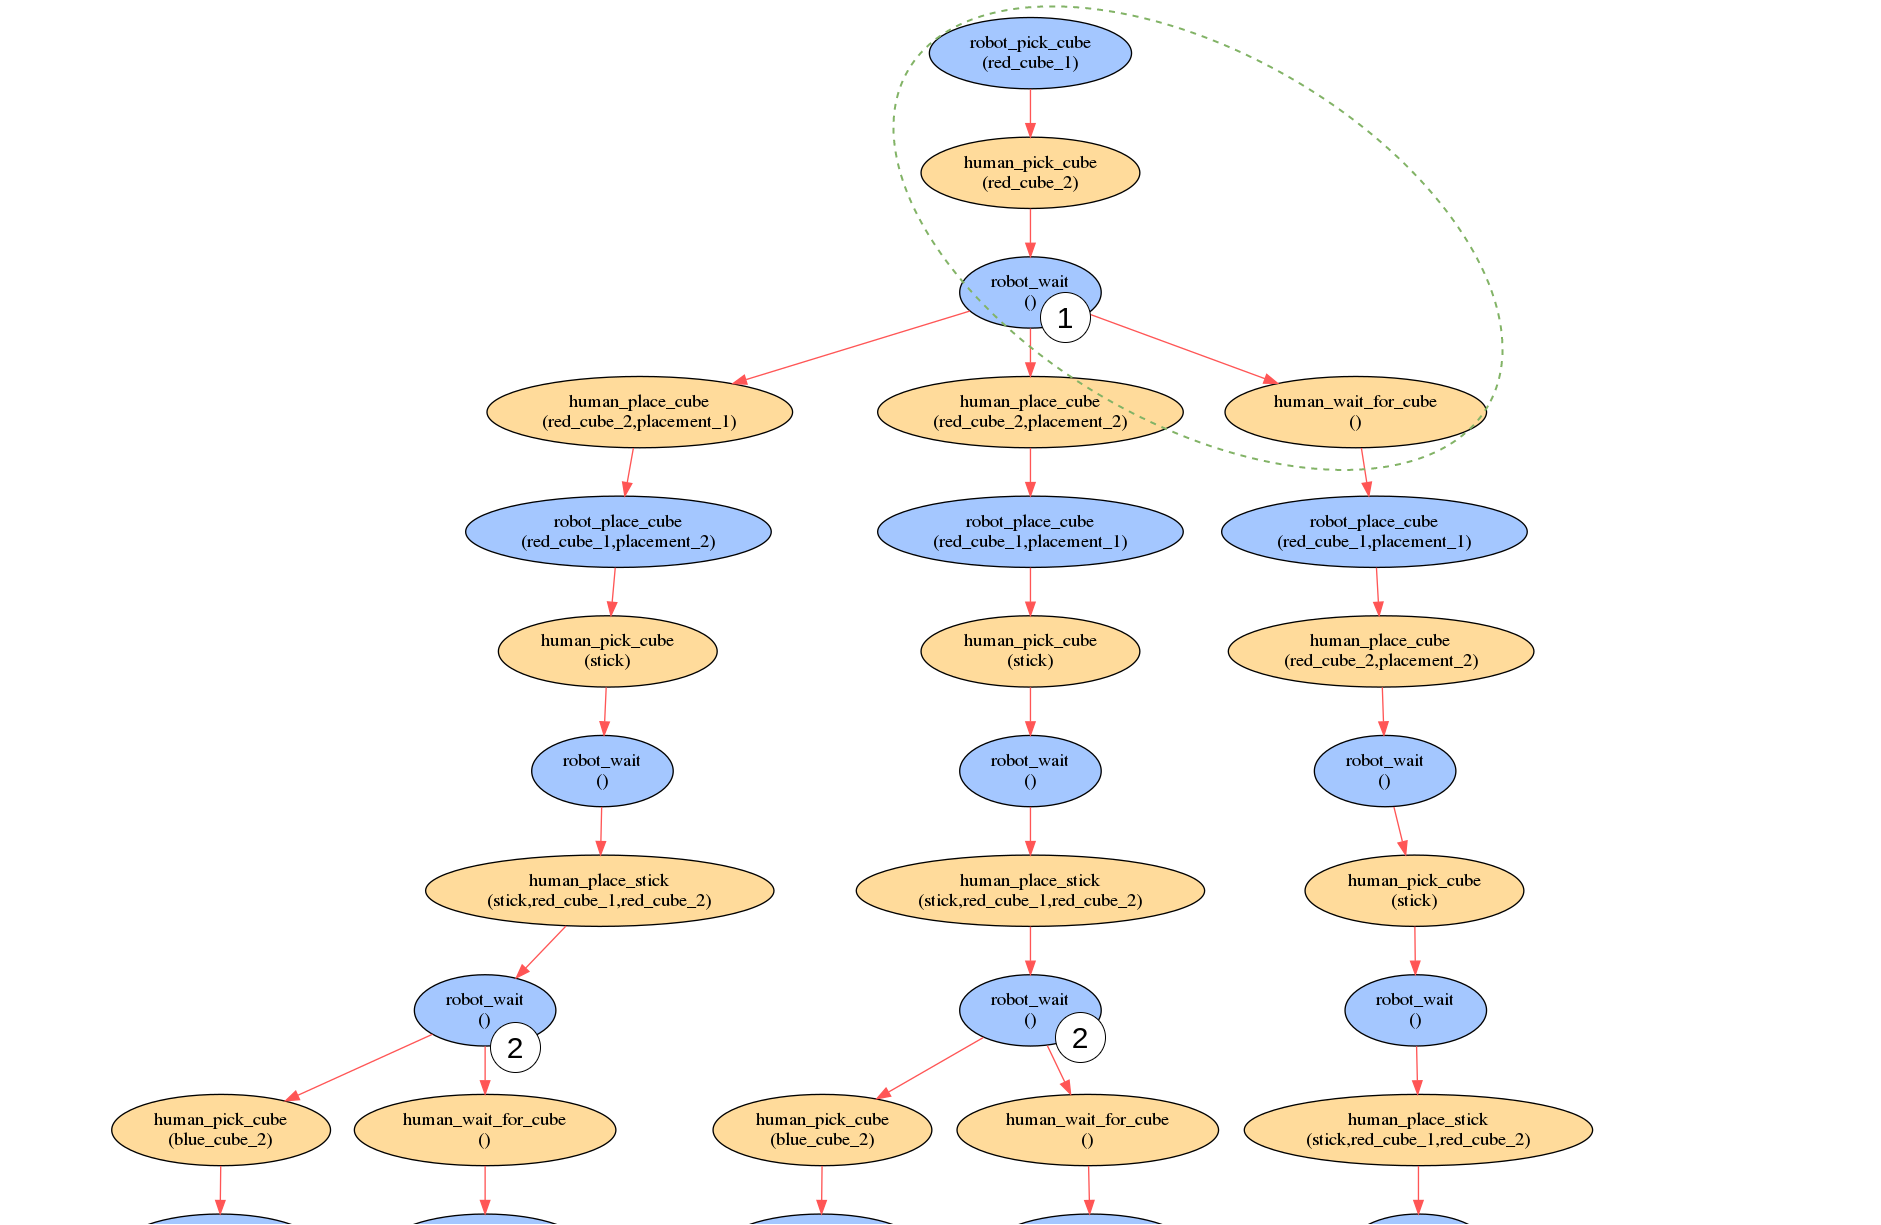
\includegraphics[scale=0.35]{figures/chapter2/plan_building.png}
	\end{figure}
\end{landscape}

\begin{landscape}
	\thispagestyle{example}
	\begin{figure}[!hp]
		\centering
		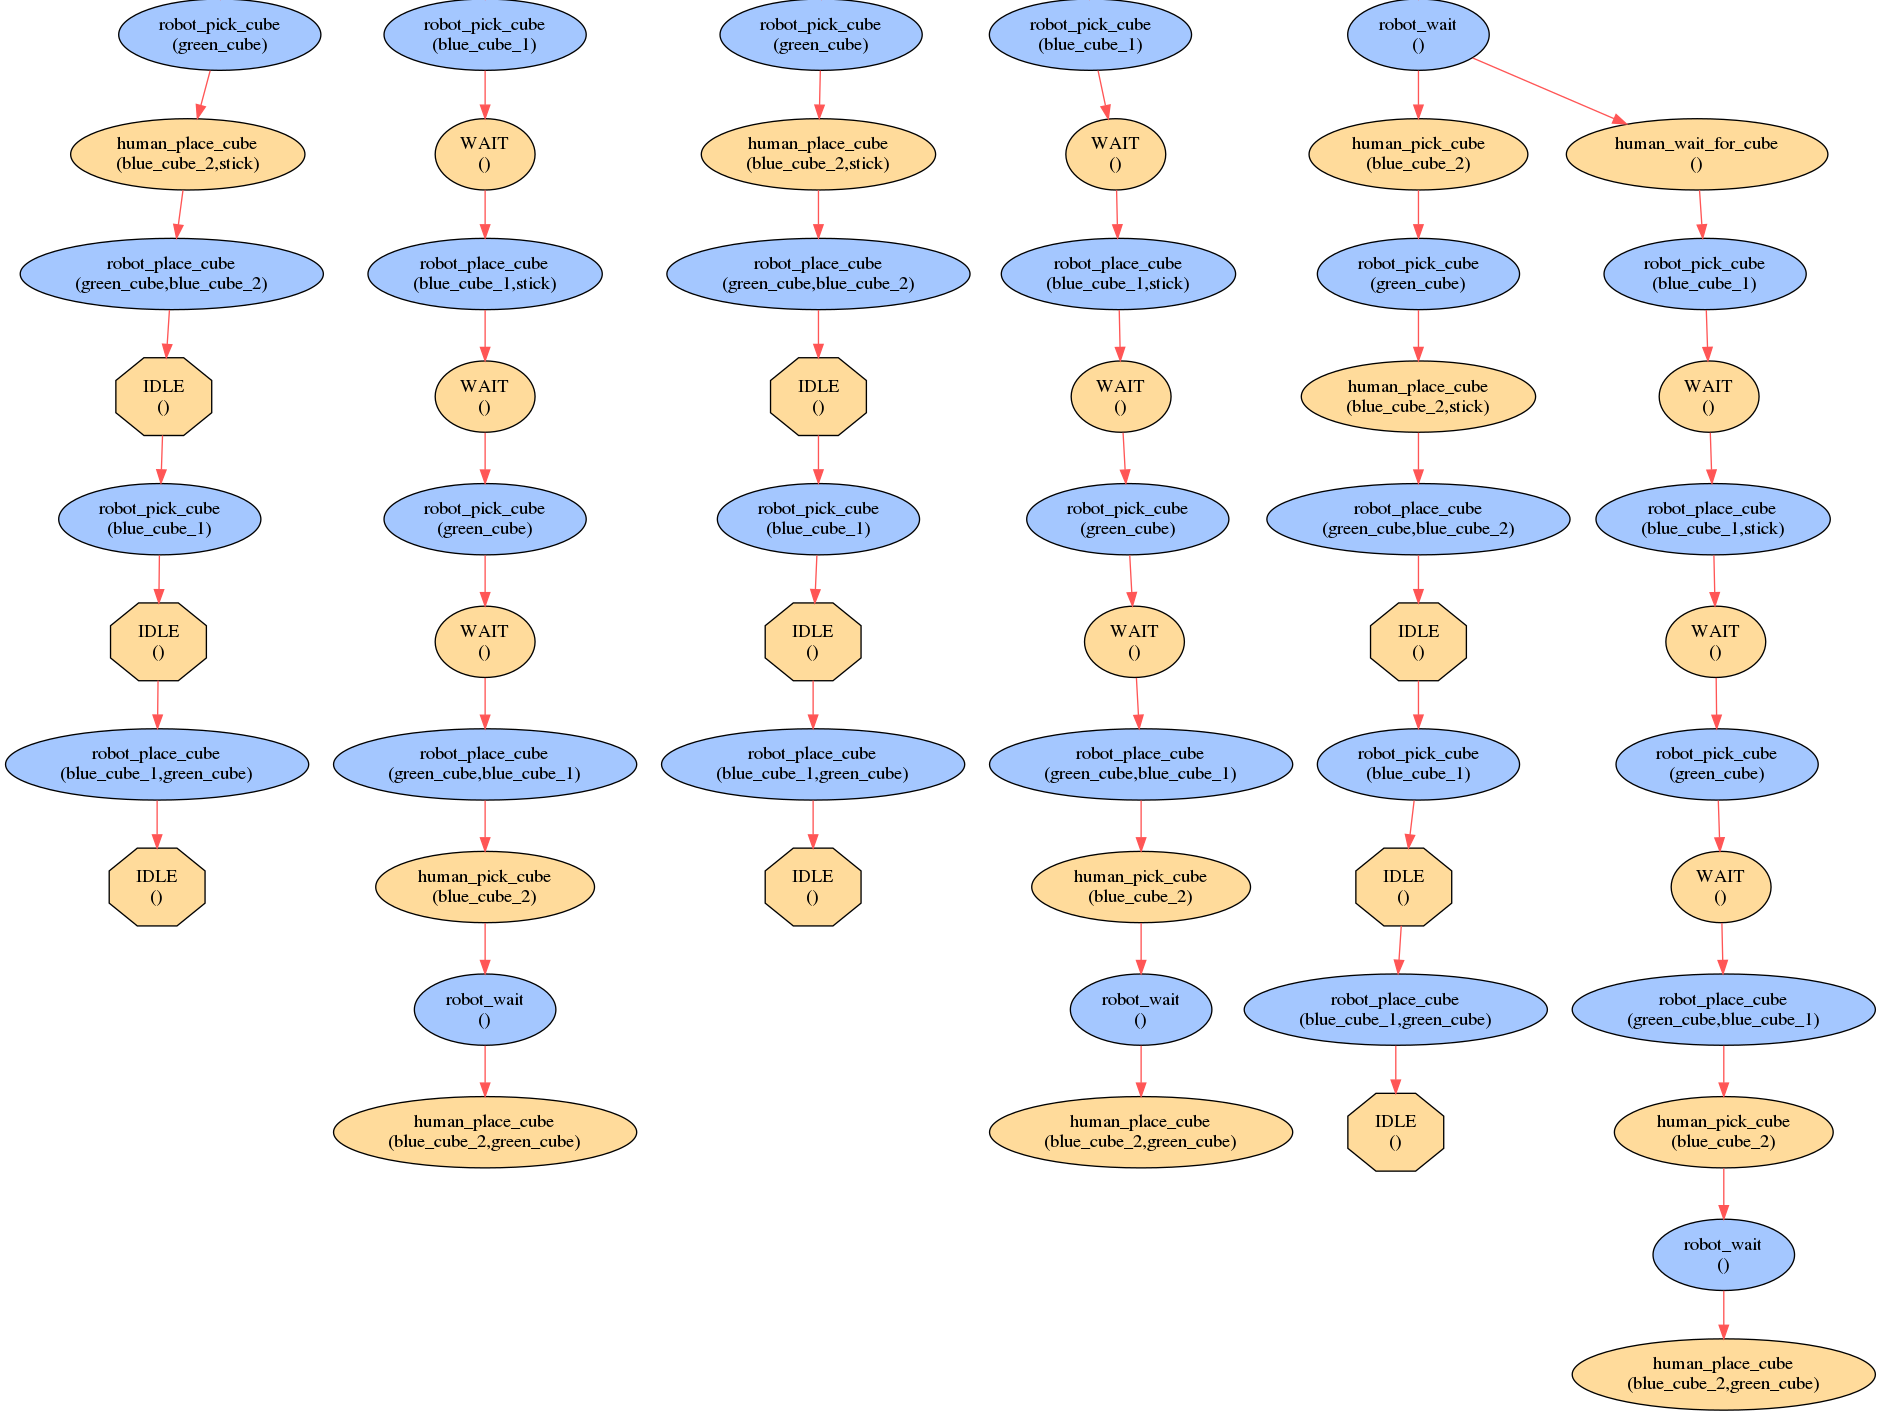
\includegraphics[scale=0.31]{figures/chapter2/plan_building2.png}
		\caption{A conditional plan for the StackBuildingTask. Twice during the task, the human has a choice. First, they can choose where to place their red cube or to wait for the robot to choose for the placement, \circledtext{1} on the figure. The second choice happens for the positioning of the first blue cube of the stack, either the human can place it on the stick or leave it to the robot, \circledtext{2} on the figure. \textit{robot\_wait}, \textit{WAIT} and \textit{IDLE} are default actions, immediately resolved as \textsc{executed} when they are \textsc{todo}. The green dotted ellipse is the plan executed in the example presented in Section~\ref{chap6:sec:example}.}
		\label{chap6:fig:plan_building2}
	\end{figure}
\end{landscape}
\restoregeometry

\bigskip
\acrshort{jahrvis} could be used to execute plans from other \acrshort{htn} planners than \acrshort{hatp} and \acrshort{hatpehda} by adding a Java class to format abstract and primitive tasks as presented in Section~\ref{chap6:subsec:shared_p_rep} -- \acrshort{hatp} and \acrshort{hatpehda} have a dedicated Java class each, for action formatting, but their plans are handled with the same code in the plan managers.

Now, we will present the two processes in charge of the shared plan management, one to handle the plan on the robot side, \ie its updates and the action execution, and the other one to handle the estimated human mental states about the shared plan. When either the robot or the human starts and finishes an action execution, facts corresponding to these events, are added to Ontologenius and Mementar to keep track of what happened during the interaction. It also registers the data about the abstract task. Then, a component of the robotic architecture used to generate communication about elements, the \acrfull{reg}, can use such information when invoked by \acrshort{jahrvis} to refer to the past (\eg ``the cube you took'').

When we will mention the robot monitoring with its head, it is done through a component described in Section~\ref{chap6:par:act_rep}.

\subsection{Robot Plan Management}\label{chap6:subsec:robot_plan}

\begin{figure}[!hbt]
	\centering
	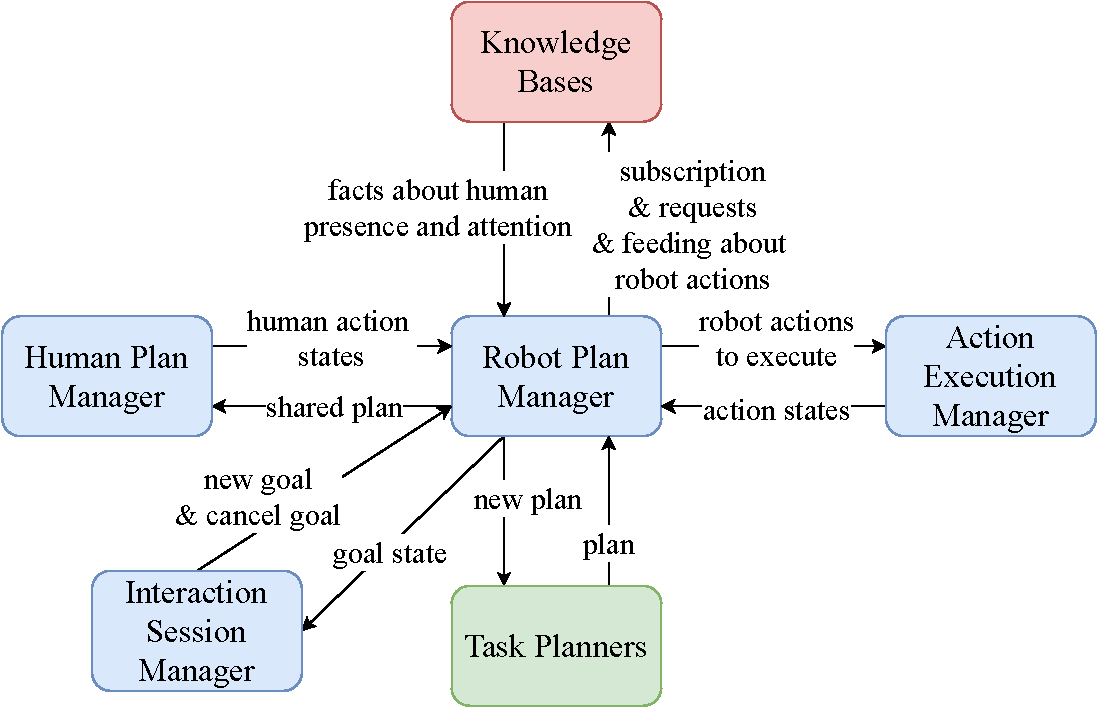
\includegraphics[width=0.85\linewidth]{figures/chapter2/robot_manager_zoom.pdf}
	\caption{The \acrlong{rpm} and the \acrshort{rja}s (in blue) and the components of the robotic architecture (in red and green) with which it interacts.}
	\label{chap6:fig:rob_manager_zoom}
\end{figure}

As explained earlier, there are two processes to manage the shared plans. One of them is the \acrfull{rpm}. It is in charge of the plan updates, maintaining the robot knowledge about the ongoing goal, and deciding which action should be performed by the robot and when. Figure~\ref{chap6:fig:rob_manager_zoom} shows its relations with the other \acrshort{rja} of \acrshort{jahrvis} and components of the robotic architecture.

\paragraph{Update of a plan}
When it receives a new goal from the \acrlong{ism}, it queries the Task Planner for a plan. This plan is a sequence of abstract and primitive tasks as described in Section~\ref{chap6:subsec:shared_p_rep}. First, when receiving the plan, and then at each end of action execution, the abstract and primitive task states of the plan are screened in order to find the next primitive task to perform. The found ones have their state set to \textsc{todo}. The implemented algorithm to do so is presented in Algorithm~\ref{chap6:algo:UP}. 

\begin{algorithm}[!htb]
	\caption{Update of a plan}
	\label{chap6:algo:UP}
	\begin{algorithmic}
		\Function{UpdatePlan}{}
		\ForEach{$\Pi_i$ with $state_i=$ \textsc{planned}}{Plan}
		\State $preds$ $\coloneqq$\textsc{FindAll}($id_j$) 
		\\\hfill such as $\Pi_j \in Plan, id_j \in preds_i,state_j\neq$ \textsc{executed} 
		\If{$preds = \emptyset$}
		\State $state_i\coloneqq$ \textsc{todo} 
		\State \textsc{UpdateAbstractTasksToOngoing($\Delta_i$)}
		\EndIf
		\EndFor
		\If{$\forall \Pi_x \in$ Plan, $state_x=$ \textsc{executed} or $state_x=$ \textsc{unplanned}}
		\State GoalState $\coloneqq$\textsc{succeeded}
		\EndIf
		\EndFunction
		\Statex
		\Function{UpdateAbstractTasksToOngoing}{$\lambda_i$}
		\If{$\exists \lambda_i$ with $state_i=$ \textsc{planned}}
		\State $state_i \coloneqq$ \textsc{ongoing} 
		\State \textsc{UpdateAbstractTasksToOngoing($\lambda_{\Delta_i}$)}
		\EndIf
		\EndFunction
	\end{algorithmic}
\end{algorithm}

\paragraph{TODO action event}
As we used Jason, a process can react to events (see Section~\ref{chap4:subsec:jason}). Every abstract or primitive task state update triggers an event. We represented what happened when a primitive task is updated to \textsc{todo} in Algorithm~\ref{chap6:algo:todo}. There are three possible cases, either an action is to be performed by the human, or the robot, or it is undefined which is represented by the AgentX. 

When an \textbf{action should be performed by the human} and if the robot does not have an action to do at the same time, the robot has to monitor them, or rather the parameters of their action, in order to be aware of what they are doing. To monitor, robot can use several modalities when they exist. Indeed, it can monitor with the camera on its head but also with a (lidar) scanner for example. As the most important thing for the \acrshort{rpm} is to monitor parameters and not how to monitor them, it sends to a component in charge of the robot resources the objects of interest for the given action. In the current state of the work, only one parameter among the parameter list is selected to be monitored. The function to select this object of interest among the action parameters is simple, we take the first of the list, but it could be refined. Or, as explained earlier, parameters can be in the form of \sparql{} queries. If it is the case, the robot chose to monitor the human closest one among the ones returned by Ontologenius. Then, it waits an update on the action state -- which is updated by the \acrfull{hpm} and then sent to the \acrshort{rpm}.


\begin{algorithm}[!htb]
	\caption{Event action todo in \acrshort{rpm}}
	\label{chap6:algo:todo}
	\begin{algorithmic}
	\Function{On}{$\Pi_i$} with $state_i=$\textsc{todo}
	\If{$agent_i \in$ Human and $name_i \in$ PhysicalAction}
	\State $objM \coloneqq$ \textsc{ChooseObjectToMonitor($params_i$)}
	\State \textsc{SetMonitorObject($objM$)}
	\State \textsc{WaitForPrimTaskStateToChange($\Pi_i$)}
	\ElsIf{$agent_i \in$ Robot or $agent_i \in$ AgentX}
		\If{$\exists p \in params_i, p$ is a \sparql{} query}
		\State $oneAgentOnly,newParams\coloneqq$ \textsc{InstantiateParams}($\Pi_i$)
		\State $params_i \coloneqq newParams$
		\EndIf
		\If{$oneAgentOnly \neq \varnothing$}
			\State $agent_i \coloneqq oneAgentOnly$ \Comment{Triggers a new \textsc{On} function as \\\hfill \textsc{todo} action updated}
		\Else
			\State \textsc{AllocatePrimTask}($\Pi_i$)
			\If{$agent_i \notin$ Human}
			 \State \textsc{SendMessage}(ActionExecutionManager,$\Pi_i$)
			 \EndIf
		\EndIf
	\EndIf
	\EndFunction
	\Statex
	\Function{InstantiateParams}{$\Pi_i$}
	\ForEach{$p$}{$params_i$}
	\If{$p$ is a \sparql{} query}
		\State $sparqlQ \coloneqq$ \textsc{SparqlToElementList($p$)} \Comment{$sparqlQ$ is a list of lists. }
		\State $oneAgentOnly = \varnothing$
		\If{$\exists a \in sparqlQ, a \in $Agent and  $a$ is unique}
			\State $oneAgentOnly \coloneqq a$
		\EndIf
		\State add $sparqlQ$ in $newParams$
	\Else
		\State add $p$ in $newParams$
	\EndIf
	\EndFor
	\State \Return $oneAgentOnly,newParams$
	\EndFunction
	\algstore{todo}
\end{algorithmic}
\end{algorithm}

When an \textbf{action should be performed by the robot or the AgentX}, first it needs to check if all action parameters are already instantiated and not a \sparql{} request. When a parameter is a \sparql{} request, it queries Ontologenius to get all the objects matching it, and eventually, the agents, in the form of a list of list. For example, if the \sparql{} request is \verb'?0 isA Cube. ?0 hasColor red', then the result could be \verb'[[red_cube_1],[red_cube_2]]'. Or, in case where there is another element in addition to the object, such as an agent, \eg \verb'?0 isA Cube. ?0 hasColor red. ?0 isReachableBy ?1', the result could be \verb'[[red_cube_1,robot],[red_cube_2,human]]'. Sometimes, an agent action is allocated to the AgentX but the environment may have changed since planning time. Then, there may be one agent only, either the human or the robot, returned in the object list (\eg \verb'[red_cube_1,robot]' if for some reason \verb'red_cube_2' is not reachable by the human anymore). In this case, the agent action value will be updated with this agent (\eg the robot). 

Next, the action has to be allocated to an agent if it is not already the case. If the agent value corresponds to the robot, the only thing to do is to select the parameters to execute the action in case some of them are object list. In the current work, the function is simple, the robot choses the first one of the list. 

If the agent value corresponds to the AgentX, then the \acrshort{rpm} checks if another action exists with the same parameters and the \textsc{todo} state. Indeed, the human cannot perform two actions at the same time so the \acrshort{rpm} can allocate one to the robot. In case there is no other action, as we think the robot as a human helper, it should leave the choice to them if they want to perform the action or not. \cite{devin_2017_decisions} showed that naive users preferred when the robot asked them what they wanted to do but \cite{macmillan_2004_communication} showed that unnecessary communication can reduce the team efficiency. Therefore, we chose the adaptive option, where the robot waits a few seconds to see if the human starts to perform the action. If they do, the action is allocated to the human and if they do not, the \acrshort{rpm} allocates the action to the robot. 

Finally, when an action is allocated to the robot, it is sent to the \acrlong{aem} that will handle the action execution as indicated by its name.


\begin{algorithm}[!htb]
	\ContinuedFloat
	\caption{Event action todo in \acrshort{rpm}(continued)}
	\begin{algorithmic}
	\algrestore{todo}
	\Function{AllocatePrimTask}{$\Pi_i$}
		\If{$agent_i \in $Robot or ($\exists \Pi_j$ with $j \neq i$, $state_j=$\textsc{todo}, $params_i=params_j$,\\\hfill $agent \in$ AgentX)} 
			\State \textsc{AllocatePrimTaskToRobot($\Pi_i$)}
		\Else
			\While{$t_{current} < T_{max\_wait}$ or \\\hfill ($state_i=$ \textsc{ongoing} or $state_i=$ \textsc{executed}) and $agent \in$ Human}\\\Comment{$\Pi_i$ state may be updated by the Human Plan Manager}
			\EndWhile
			\If{$agent \notin$ Human}
				\State \textsc{AllocatePrimTaskToRobot($\Pi_i$)}
			\EndIf
		\EndIf
	\EndFunction
	\Statex
	\Function{AllocatePrimTaskToRobot}{$\Pi_i$}
	\ForEach{$p$}{$params_i$}
		\State \textsc{SelectParams($params_i$)}
		\State $agent_i \coloneqq$ Robot
	\EndFor
	\EndFunction
	\end{algorithmic}
\end{algorithm}

\thispagestyle{example}
\paragraph{EXECUTED action event}
We represented what happened when a primitive task is updated to \textsc{executed} in Algorithm~\ref{chap6:algo:executed}. As explained above, the manipulated plans can be conditional plans. Thus, at the end of each action execution, the \acrshort{rpm} looks if at place of the plan, the human had the choice between the action they just executed and other actions. If it is the case, these other actions and all their descendants are set to \textsc{unplanned} as they should not be executed. For example, let's look at the \acrshort{hatpehda} plan in Figure~\ref{chap6:fig:plan_building2} and the first choice the human can do. The robot detected that the human placed their red cube on \verb'placement_1'. Thus, the action with them placing the cube on  \verb'placement_1', and the one where they wait, as well as the all the other abstract and primitive tasks of these two branches, are not part of the plan anymore. 

\thispagestyle{example}
Then, the plan is updated to find the next actions \textsc{todo} as presented in Algorithm~\ref{chap6:algo:UP}.
%To do so, it tries to find if the agent and the predecessor of the action which just finished are the same than the ones of another action. If it is the case, all the abstract and primitive task descendant of this found action are set \textsc{unplanned}.

\begin{algorithm}[!htb]
	\caption{Event action executed in \acrshort{rpm}}
	\label{chap6:algo:executed}
	\begin{algorithmic}
	\Function{On}{$\Pi_i$ with $state_i=$\textsc{executed}}
		\State \textsc{EndObjectMonitoring($params_i$)}
		\State \textsc{RemoveParallelBranches($agent_i$,$preds_i$)}
		\State \textsc{UpdateAbstractTaskState($\Delta_i$,\textsc{executed})}
		\State \textsc{UpdatePlan} \Comment{see Algorithm~\ref{chap6:algo:UP}}
	\EndFunction
	\Statex
	\Function{RemoveParallelBranches}{$agent_i$,$preds_i$}
		\State $primTasksToUnplan \coloneqq$ \textsc{FindAll}($\Pi_x$) \\\hfill with $agent_x=agent_i, preds_x=preds_i,$ \\\hfill$(state_x=$ \textsc{todo} or $state_x=$ \textsc{suspended})
		\State \textsc{RemovePrimTasks}($primTasksToUnplan$)
	\EndFunction
	\Statex
	\Function{RemovePrimTasks}{$primTasksToUnplan$}
		\ForEach{$\Pi_i$}{$primTasksToUnplan$}
			\State $state_i\coloneqq$ \textsc{unplanned} 
			\State \textsc{UpdateAbstractTaskState($\Delta_i$,\textsc{unplanned})}
			\State \textsc{RemoveChild($\Pi_i$)}
		\EndFor
	\EndFunction
	\Statex
	\Function{RemoveChild}{$\Pi_i$}
		\State $primTasksToUnplan \coloneqq$ \textsc{FindAll}($\Pi_j$) with $id_i \in preds_j$ 
		\State \textsc{RemovePrimTasks}($primTasksToUnplan$)
	\EndFunction
	\Statex
	\Function{UpdateAbstractTaskState}{$id_x$,$newState$}
		\If{$ \forall \lambda_i$,$\Pi_i$ with $\Delta_i=id_x$, ($state_i=$ \textsc{executed} or $state_i=$ \textsc{unplanned})}
			\State $state_x \coloneqq newState$
			\State \textsc{UpdateAbstractTaskState($\Delta_x$,$newState$)}
		\EndIf
	\EndFunction	
	\end{algorithmic}
\end{algorithm}		

\clearpage
\subsection{Human Plan Management}\label{chap6:subsec:human_plan}

\begin{figure}[!hbt]
	\centering
	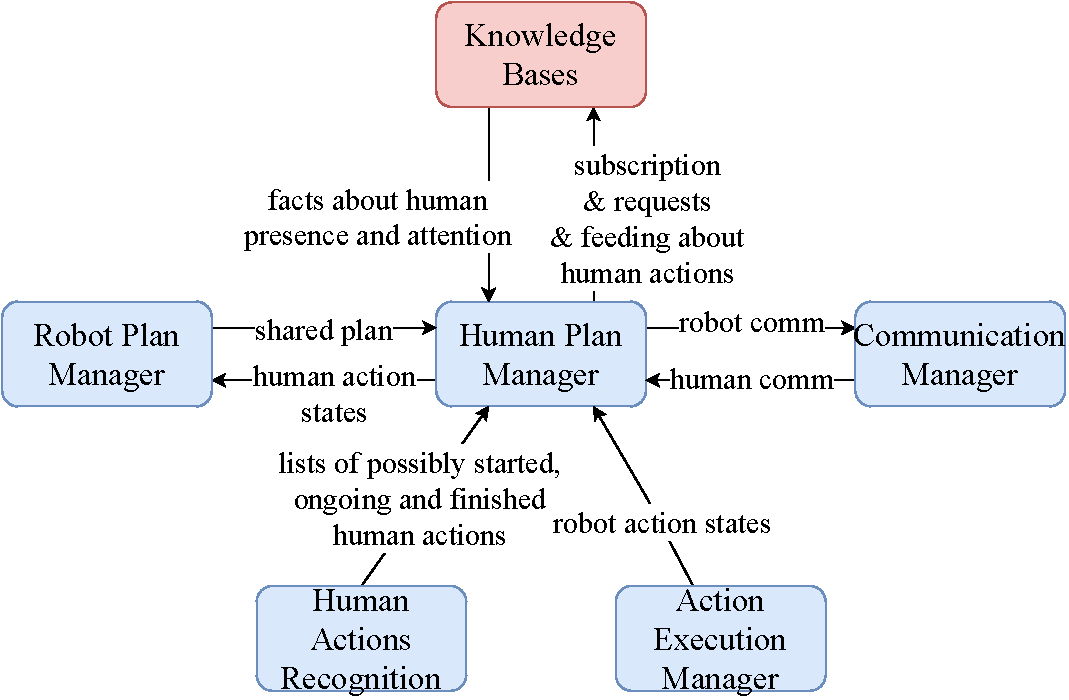
\includegraphics[width=0.85\linewidth]{figures/chapter2/human_manager_zoom.pdf}
	\caption{The \acrlong{hpm} and the \acrshort{rja}s (in blue) and the component of the robotic architecture (in red) with which it interacts.}
	\label{chap6:fig:human_manager_zoom}
\end{figure}

The \acrfull{hpm} keeps track of the estimated human mental state about the ongoing shared plan, endowing the robot with \acrlong{tom} (see Section~\ref{chap1:sec:tom}). The role of this process is central, as it receives the data about the recognized human actions, deduces what the human might or might not know about the plan or action executed by the robot, and requests the communication to perform to the \acrfull{cm}. Figure~\ref{chap6:fig:human_manager_zoom} shows its relations with the other \acrshort{rja} of \acrshort{jahrvis} and components of the robotic architecture.

When a shared goal starts, it receives from the \acrshort{rpm} the list of primitive tasks composing the plan. The action states are updated with the same algorithm as the \acrshort{rpm}, Algorithm~\ref{chap6:algo:UP} (with the function updating the abstract tasks being not used). We distinguish two cases of \textsc{todo} actions, the actions to be performed by the human and the ones to be performed by the robot.

\paragraph{Action to be performed by the human} We present Algorithm~\ref{chap6:algo:h_todo}, describing what happens in the~\acrshort{hpm} when it computes that the human has an action to perform, with effects that are VisualEffects (see Section~\ref{chap6:subsec:action_rep}). It only shows when everything goes well, \ie that the human performs the right action in the allocated time. The way the robot reacts if the human is not acting, by communicating, is described with Algorithm~\ref{chap6:algo:h_todo_conting_1} for the case where the action never started and with Algorithm~\ref{chap6:algo:h_todo_conting_2} for the case where the robot detected the start but cannot see the final action effects.

As we can see in Algorithm~\ref{chap6:algo:h_todo}, when the \acrshort{hpm} estimates the human is aware that they have an action to perform, it checks if action data received from the \acrlong{ham} matches it. The function comparing the \textsc{todo} action with monitored actions communicated by the \acrshort{ham} is a Jason rules, comparing the agent names, the action classes and the parameters. If the \textsc{todo} action has \sparql-like parameters, the rule allows to check if it can correspond to the parameters of a given recognized action. Moreover, because \acrshort{jahrvis} enables the use of conditional plan where the branch choices are made by the human, when the human makes one of this choice, the other branches have to be \textsc{suspended} and then \textsc{unplanned}.

\begin{algorithm}[!htb]
	\caption{Event action todo by human in \acrshort{hpm}}
	\label{chap6:algo:h_todo}
	\begin{algorithmic}
	\Function{On}{$\Pi_i$} with $agent_i \in$ Human and $state_i=$ \textsc{todo}
	\State $matchingAction \coloneqq false$
	\While{$t_{current} < T_{timeout,start}$ and not $matchingAction$}
		\If{\textsc{Match}($\Pi_i$,$monitoredAction_{\text{STARTED,PROG,ACHIEV}})$}
		\State $matchingAction \coloneqq true$
		\EndIf
	\EndWhile
	\If{$t_{current} > T_{timeout,start}$} \Return \EndIf
	\If{\textsc{Match}($\Pi_i$,$monitoredAction_{\text{STARTED,PROG}})$}
	\State $state_i \coloneqq$ \textsc{ongoing}
	\State \textsc{SendMessage}(RobotPlanManager,$\Pi_i$)
	\State $matchingAction \coloneqq false$
	\EndIf
	\State $primTasksToSuspend \coloneqq$ \textsc{FindAll}($\Pi_j$) with $id_i \in preds_j$ 
	\State \textsc{SuspendPrimTasks}($primTasksToSuspend$)
	\While{$t_{current} < T_{timeout,achiev}$ and not $matchingAction$}
		\If{\textsc{Match}($\Pi_i$,$monitoredAction_{\text{ACHIEV}})$}
		\State $matchingAction \coloneqq true$
		\EndIf
	\EndWhile
	\If{$t_{current} > T_{timeout,achiev}$} \Return \EndIf
	\State  $state_i \coloneqq$ \textsc{executed} 
	\State \textsc{SendMessage}(RobotPlanManager,$\Pi_i$)
	\State \textsc{RemoveParallelBranches}(human,$preds_i$) \Comment{see Algorithm~\ref{chap6:algo:executed}}
	\State \textsc{UpdatePlan} \Comment{see Algorithm~\ref{chap6:algo:UP}}
	\EndFunction	
	\end{algorithmic}
\end{algorithm}	

When the robot estimates that the human knows they should perform an action but this does not happen, it initiates a communication through the \acrlong{cm} in order to indicate to the human that they have this given action to do. Thus, it updates once again its estimation of the human mental state about the action, setting it to \textsc{todo} since it informed them. It is described by Algorithm~\ref{chap6:algo:h_todo_conting_1}.

\begin{algorithm}[!htb]
	\caption{Handling of action todo timed out on wait for started/progressing action by human in \acrshort{hpm}}
	\label{chap6:algo:h_todo_conting_1}
	\begin{algorithmic}
		\Function{NotDoing}{List of $\Pi$ with $state=$ \textsc{todo}}
		\If{first time for these actions}
			\ForEach{$\Pi_i$}{List of  $\Pi$}
			\State $state_i\coloneqq$ \textsc{not\_starting} 
			\EndFor
			\State \textsc{SendMessage}(CommManager,List of primTask)
			\ForEach{$\Pi_i$}{List of $\Pi$}
			\State$state_i\coloneqq$ \textsc{todo} 
			\EndFor
		\Else
			\State \textsc{Negociation} or \textsc{StopGoal} \Comment{Negociation not implemented}
		\EndIf
		\EndFunction
	\end{algorithmic}
\end{algorithm}		

A bit similarly, when the robot observed the beginning of an action, it asks the human if they did it, as it might have missed the end of the action execution and/or for some reason might not be seeing the action necessary effect. If the human answers yes, the robot updates the action state as well as the actions effects in Ontologenius. In the other case, the robot set the action to \textsc{todo} as the human knows they should do it. This function could be enhanced with a more sophisticated dialog. 
			
\begin{algorithm}[!htb]
	\caption{Handling of action todo timed out on wait for achieved action by human in \acrshort{hpm}}
	\label{chap6:algo:h_todo_conting_2}
	\begin{algorithmic}
		\Function{NotDoing}{$\Pi_i$} with $agent_i \in$ Human and $state_i=$ \textsc{todo}
		\If{first time for this actions}
			\State $state_i\coloneqq$ \textsc{not\_finished} 
			\State $answer \coloneqq$ \textsc{SendMessage}(CommManager,$\Pi_i$)
			\If{$answer=$ no}
				\State $state_i\coloneqq$ \textsc{todo} 
			\Else
				\State $state_i\coloneqq$ \textsc{executed} 
				\State \textsc{UpdateOntologenius($necessEffectL_i$)}
			\EndIf
		\Else
			\State \textsc{Negociation} or \textsc{StopGoal}
		\EndIf
		\EndFunction
	\end{algorithmic}
\end{algorithm}		

Sometimes, it can happen that the \acrshort{hpm} receives from the \acrshort{ham} that a human action has been achieved whereas no human primitive task is in a \textsc{todo} state. This recognized action might be matching a \textsc{planned} action which would have been the next to be set to \textsc{todo}. Such a situation arises because \acrshort{hatpehda} is still a prototype and does not give the causal links between actions. Then currently, we can see the human performing an action which preconditions are met whereas in the plan it appears after a given robot action not executed yet. In a plan with causal links, this type of action would be parallel to the robot action and not following. But, meanwhile we are waiting for a planner update, we implemented the handling of such a case. If this happens, the primitive task is set to \textsc{executed} and the plan state is updated with Algorithm~\ref{chap6:algo:UP}.

Moreover, as we can see in the plan represented in Figure~\ref{chap6:fig:plan_building2}, the human has sometimes \verb'WAIT' actions allocated to them in the plan. Contrarily to \verb'IDLE' for situations in which the human cannot act without the robot action or has finished their part of the plan, the human can be acting during \verb'WAIT' actions, performing their next non-wait action. Indeed, it is also a case where causal links should be used. Thus, we circumvented the issue by checking if a human recognized action matches an action following \verb'WAIT' actions in the plan. If so, the action is set to \textsc{executed} and the plan state is updated with Algorithm~\ref{chap6:algo:UP}.

Finally, if a human action recognized as achieved but does not match the two situations explained in the previous paragraphs, the \acrshort{hpm} requests a replanning to the \acrshort{rpm}.


\paragraph{Action to be performed by the robot} Now, the \acrshort{hpm} should also handle when an action is to be performed by the robot. Thanks to the class action we defined (see Section~\ref{chap6:subsec:action_rep}), actions on the environment and communication actions can be process differently. For the latter, human attention is monitored by the \acrlong{cm}. 

The handling of an action performed by the robot depends on the estimated establishment of a (simple) joint attention (see Section~\ref{chap1:subsubsec:joint_att}) between the human and the robot. An activity diagram presented in Figure~\ref{chap6:fig:robot_action_hpm} shows that when the \acrshort{hpm} is informed by the \acrfull{aem} of a robot ongoing action, it monitors, if the human is in its field of view, their attention towards the action parameters or the robot. When the \acrshort{hpm} estimates that the human sees what is going on, then it updates the human's mental state about this action. When it estimates that they have not seen the action, then it considers that the human has a false belief about the action, as in the robot's belief base the action is executed but not in the human's one, there is a belief divergence (see Section~\ref{chap1:sec:tom}). Thus, it communicates to realign the human's beliefs. Moreover, even if the robot was in the human's field of view (FoV), sometimes some action effects are non-observable (see Section~\ref{chap6:subsec:action_rep}), so this is another case where the robot will communicate about an action it executed. Then, when an action is set as \textsc{executed} in the human's mental state, it updates the plan with the function presented in Algorithm~\ref{chap6:algo:UP}.

\begin{figure}[!ht]
	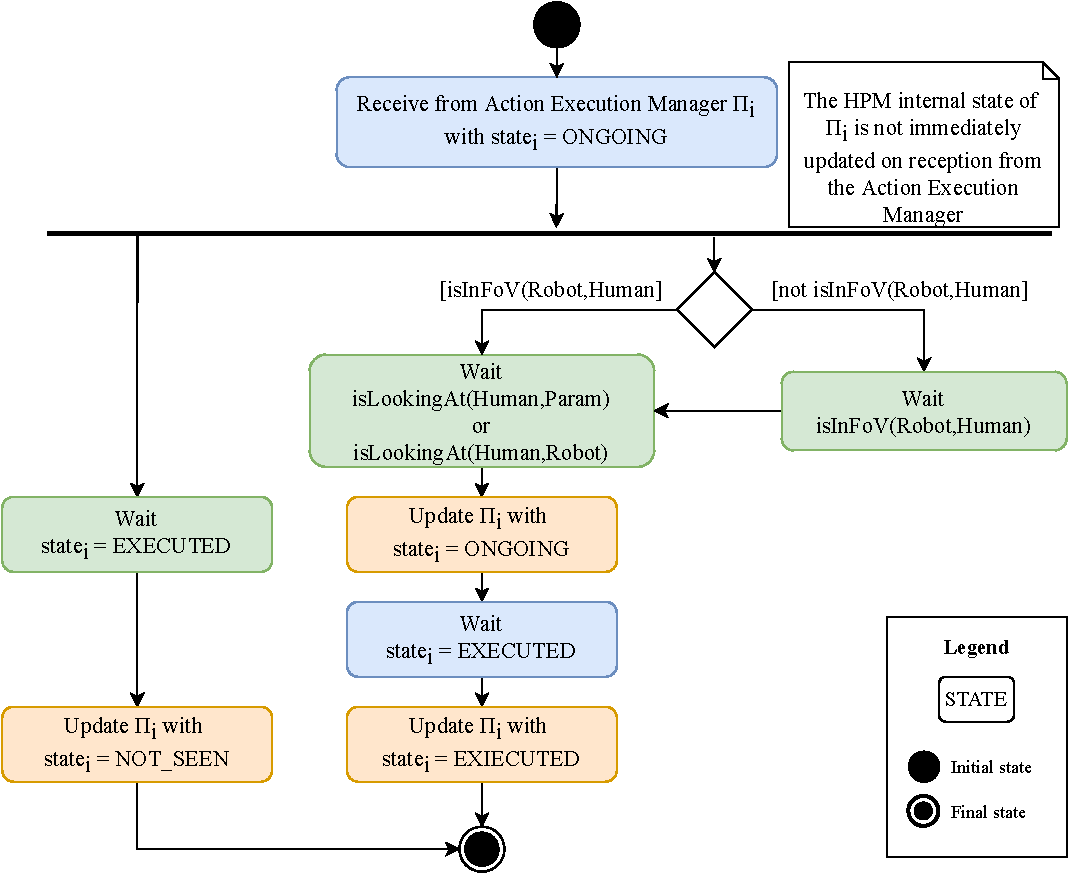
\includegraphics[width=\linewidth]{figures/chapter2/robot_action_hpm.pdf}
	\caption{Activity diagram representing what happens when the \acrfull{aem} sends to the \acrshort{hpm} that the robot started to execute an action. We represent in blue the nodes receiving data from the \acrshort{aem}, in green the ones receiving data from Ontologenius and in orange the ones updating the action state in the \acrshort{hpm} belief base.}
	\label{chap6:fig:robot_action_hpm}
\end{figure}

\clearpage

\section{Action Execution Management}\label{chap6:sec:aem}

\begin{figure}[!hbt]
	\centering
	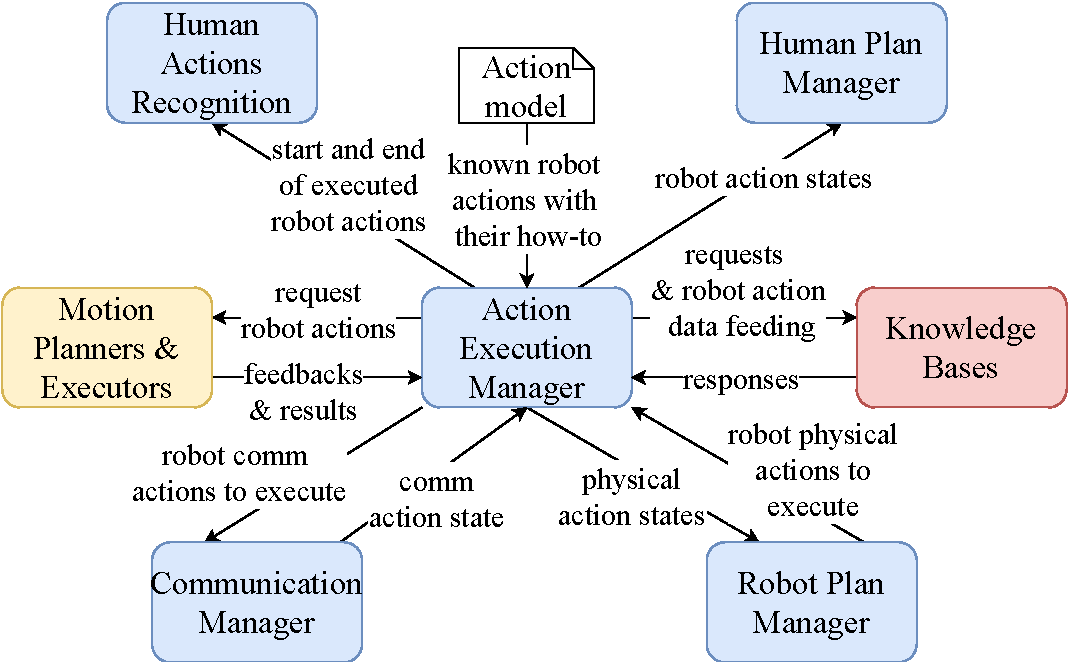
\includegraphics[width=0.85\linewidth]{figures/chapter2/action_exe_manager_zoom.pdf}
	\caption{The \acrlong{aem} and the \acrshort{rja}s (in blue) and the components of the robotic architecture (in red and yellow) with which it interacts. It is fed by a file (in white) with description of the robot actions the robot can do and how.}
	\label{chap6:fig:action_exe_zoom}
\end{figure}

Deciding is not enough, the robot needs to be able to act. Thus, \acrshort{jahrvis} has a \acrfull{rja} called the \acrfull{aem}. Figure~\ref{chap6:fig:action_exe_zoom} shows its relations with the other \acrshort{rja} of \acrshort{jahrvis} and components of the robotic architecture. The \acrshort{aem} is composed of a generic part managing the general flow of an action execution, described in Algorithm~\ref{chap6:algo:exe_manage}, and of a task-specific part, specifying the distinctive characteristic of given actions which are instantiations of the \textsc{Execute} function in a separate ASL file as explained in Section~\ref{chap6:par:act_rep}. Moreover, all actions of the type PhysicalAction are realized based on action clients to communicate with the Motion Planners and Executors (see Figure~\ref{chap3:fig:archi}) which allows a fine management of the execution through feedbacks and error codes. Finally, each instantiation of a PhysicalAction automatically starts and ends with the setting of the action parameters monitoring by the robot head, based on the head management presented in the next paragraph. For CommunicateAction, their parameters are reorganized and then the action is sent to the \acrshort{cm} for execution. 

\begin{algorithm}[!htb]
	\caption{Action execution management}
	\label{chap6:algo:exe_manage}
	\begin{algorithmic}
	\Function{ExecuteAction}{$\Pi_i$} with $agent_i \in$ Robot
	\If{$name_i \in$ PhysicalAction}
		\State \textsc{SendMessage}([\acrshort{rpm},\acrshort{hpm},\acrshort{ham}], $\Pi_i$) with $state_i=$ \textsc{ongoing}
	\ElsIf{$name _i \in$ CommunicateAction}
		\State \Comment{\textsc{ongoing} state set by the \acrshort{cm}}
		\State \textsc{SendMessage}(CommManager,$\Pi_i$) with $state_i=$ \textsc{todo}
	\EndIf
	\State $action \coloneqq$ \textsc{ActionParsing($name_i$,$params_i$)}
	\State \textsc{Execute($action$)}
	\If{$name_i \in$ PhysicalAction}
		\State \textsc{SendMessage}([\acrshort{rpm},\acrshort{hpm},\acrshort{ham}], $\Pi_i$) with $state_i=$ \textsc{executed}
	\ElsIf{$name \in$ CommunicateAction}
		\State \textsc{SendMessage}([\acrshort{rpm},\acrshort{hpm}], $\Pi_i$) with $state_i=$ \textsc{executed}
	\EndIf
	\EndFunction
	\end{algorithmic}
\end{algorithm}	



\paragraph{Robot Resource Management}\label{chap6:para:resource_m}

The correct handling of the resources (head, arms, base...) of a robot is critical to perform a task, but it can be cumbersome for a deliberative component, such as \acrshort{jahrvis}, to do all the micro-management required. To tackle this issue, a physical resource management system has been designed by Guillaume Sarthou and Guilhem Buisan, inspired by \cite{devin_2017_decisional}. For each of the identified resources is instantiated a component called \emph{Resource Manager}, having two types of input: permanent channels, that can be preempted at any time (\eg look at the head of the human interacting with it) and finite state machines which are not preemptable (\eg set of commands to scan a table). A component called \emph{Resource Synchronizer} deals with actions requiring multiple resources such as the human-aware navigation which uses the head and the base. The synchronizer also reports the status of the ongoing coordination signal to \acrshort{jahrvis} to monitor the progress of the action. Finally, a priority scheme has been implemented to handle multiple active inputs at the same time for one resource. 

Such component allows \acrshort{jahrvis} to be agnostic about the used robotic platform, as it offers the same interface for whichever one. Moreover, it enables joint attention with a nice head control as \acrshort{jahrvis} can switch priorities between three types of permanent channels that have been defined, depending on where we are in the task: environment monitoring, human head monitoring and human hand monitoring. The two latter are set with the head and hand of the human the robot is interacting with as point to follow, whereas the environment monitoring channel receives new point of focus according to the needs of the task (\eg the cube the robot should pick or the box in which the human has to put an object). Thus, when the agents are talking together, \acrshort{jahrvis} will set the human's head with the highest priority, but when the robot has to pick a cube, it will be the environment monitoring that will have priority. Finally, the head behavior can be controlled not only based on visual inputs but also on laser inputs for example if it has some. Indeed, according to the task context, it can be interesting for the robot to know what is going on around it. In this case, a channel can be instantiated so the robot can react when it detects moves with its laser and then looks in this direction.

\section{Communication Management}\label{chap6:sec:comm}

\begin{figure}[!hbt]
	\centering
	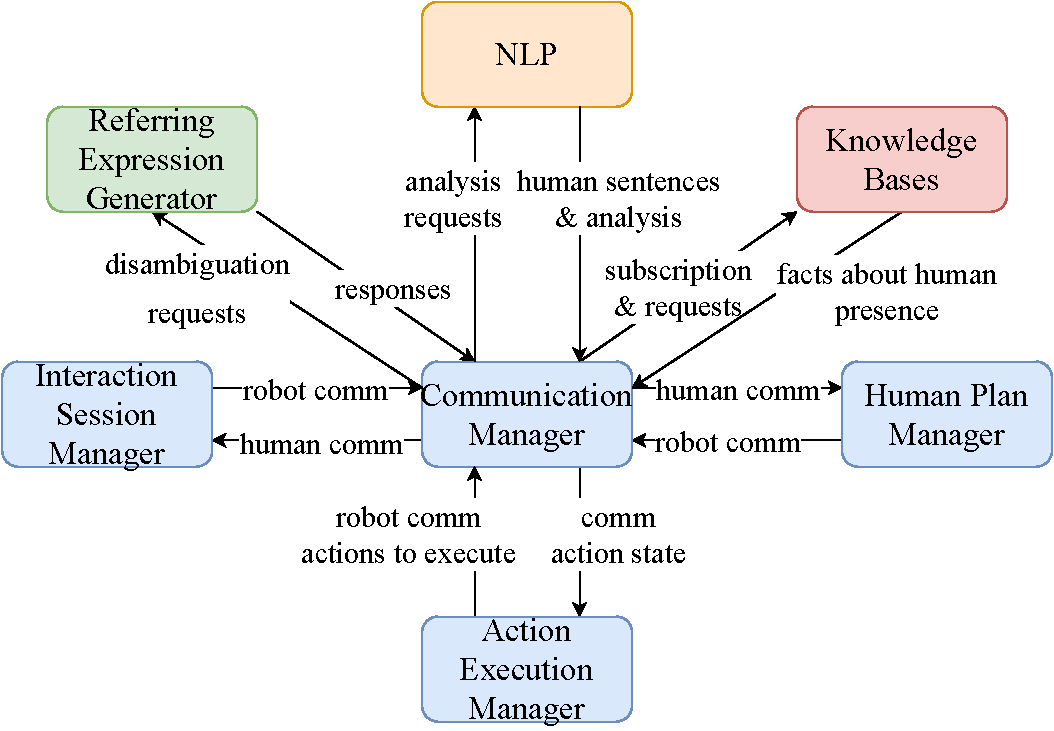
\includegraphics[width=0.85\linewidth]{figures/chapter2/comm_manager_zoom.pdf}
	\caption{The \acrlong{cm} and the \acrshort{rja}s (in blue) and the components of the robotic architecture (in red, green and orange) with which it interacts.}
	\label{chap6:fig:comm_manager_zoom}
\end{figure}

The last \acrshort{rja} involved in the robot decision and control is the \acrfull{cm}. It is not dedicated to complex talks with the human but to enable the robot to perform and interpret communication during collaborative tasks, because as shown in Section~\ref{chap1:sec:comm}, it is important. This process is based on a software for Natural Language Processing (NLP) and closely linked to a domain-specific planner called \acrfull{reg}. This latter has been developed by Guillaume Sarthou and Guilhem Buisan~\citep{buisan_2020_efficient, sarthou_2021_extending}. It aims, regarding the current symbolic state of the world, at finding the minimal set of relations to communicate and allows, when interpreting a communication, to identify a given entity. For example, if the robot wants to talk about a green cube on a table but there is another green one on a close shelf and a red cube on the table, how can it do? Well, it queries the \acrshort{reg} which answers with a nominal group such as ``the green cube on the table''. Figure~\ref{chap6:fig:comm_manager_zoom} shows its relations with the other \acrshort{rja} of \acrshort{jahrvis} and components of the robotic architecture.


\subsection{What information to communicate? How to communicate it and when?}\label{chap6:subsec:info_comm}
As shown above, three other processes, the \acrlong{ism}, the \acrlong{hpm} and \acrlong{aem}, can query the \acrshort{cm} to issue a communication to the human. We defined several types of verbal communicative acts the robot can do:
\begin{enumList}
	\item to do social chat for interaction session opening and closing (\eg ``hello''),
	\item to give information about its abilities/role (\eg ``I'm here to help you find your way''),
	\item to initiate a shared goal (\eg ``Let's do this package''),
	\item to give information about the ongoing task (\eg ``I cleaned the table''),\label{chap6:emum:comm1}
	\item to ask information about the ongoing task (\eg ``Have you cleaned the table?''),
	\item to request the human to perform an action (\eg ``Can you clean the table?''), and\label{chap6:emum:comm2}
	\item to give up the shared goal (\eg ``I'm sorry I give up, I'm failing'')
\end{enumList}

We focus on the communicative acts \ref{chap6:emum:comm1} and \ref{chap6:emum:comm2} with the verbalization of actions presented in Algorithm~\ref{chap6:algo:action_verba}, developed in collaboration with Guillaume Sarthou. 

As the communication is important, it is essential to minimize the risk that it gets lost. Thus, when the \acrshort{cm} receives a communication to perform from another \acrshort{rja}, it ensures that it perceives the human before issuing the communication, so it has more chance to get the human's attention. Therefore, it sets the monitoring channel of the Robot Resource Manager on the human head monitoring (see Section~\ref{chap6:para:resource_m}).

Moreover, when the robot needs to inform the human that it executed a given action or to ask them to perform one, it needs to verbalize it properly. Still in the spirit of a generic system, the algorithm that we developed is not task or action specific. Action labels (presented in Section~\ref{chap6:subsec:action_rep} and verb conjugation) are stored in Ontologenius which can be manually fed with new ones when needed.

Let's take an example where instead of making a stack, the agents have to remove the cubes from the table to put them in a green box. Then, we put ourselves in the case where the robot informs the human it has performed a Drop action \verb'robot_drop_cube' in the plan, with \verb'red_cube_1' and \verb'green_box' as parameters. 

First, the \acrshort{cm} queries Ontologenius to get the closest class in the hierarchy with labels. Here, it is \verb'DropAction'. There are three possible labels for this action, so the robot has the possibility to communicate about it with different action parameters: \verb'[{Agent} @Drop {Cube},' \verb'{Agent} @Drop in {Container},' \verb'{Agent} @Drop {Cube} in {Container}]'. Thus, the \acrshort{cm} finds which label matches its parameters, based on the parameter number and on their class. Then, in our case, this is \verb'{Agent} @Drop {Cube} in {Container}'. 

Next, for each parameter, it tries to find the right verbalization, either it will be a Referring Expression or the parameter label stored in Ontologenius, and replace them in the class action label. So, we would have something like \verb'{Agent} @Drop the red cube on the table in the box'. 

Finally, it replaces \verb'{Agent}' with the action actor and \verb'@Drop' with the right conjugation. As the \acrshort{cm} wants to refer to an action the robot has done, it queries the Ontology with the conjugation of \verb'Drop' at the past first singular person, which is \verb'dropped'. Then, the result of the action verbalization is \verb'I dropped the red cube on the table in the box'. 

When the \acrshort{cm} wants to ask the human to perform an action, it uses the same algorithm and turn the sentence into an interrogative form with the verb ``can''. As \acrshort{jahrvis} manipulates conditional plans, the \acrshort{cm} can take as input list of actions and separate them with ``or'' when communicating about them. And, when it wants to communicate about the human having to perform several actions in a row, it uses ``and''.
 
\begin{algorithm}[!htb]
	\caption{Action verbalization}
	\label{chap6:algo:action_verba}
	\begin{algorithmic}
	\Function{ActionVerbalization}{$agent$,$action$,$parameters$,$tense$}
	\State $labelList \coloneqq$\textsc{GetClassActionLabels($action$)}\Comment{Query to Ontologenius}
	\State $actionVerba \coloneqq$\textsc{LabelToWords}($labelList$,$parameters$)
	\If{$agent \in$ robot}
		\State $person \coloneqq$ FirstSingularPersonalForm
		\State $pronoun \coloneqq$ I
	\ElsIf{$agent \in$ human}
		\State $person \coloneqq$ SecondSingularPersonalForm
		\State $pronoun \coloneqq$ you
	\EndIf
	\State $verb \coloneqq$\textsc{GetVerb}($actionVerba$)
	\State $conjugatedVerb \coloneqq$\textsc{GetConjug}($actionVerba$,$verb$,$person$,$tense$)\Comment{Query to \\\hfill Ontologenius}
	\State $actionVerba \coloneqq actionVerba.$\textsc{Replace}(``\{Agent\}'',$pronoun$)
	\State $actionVerba \coloneqq actionVerba.$\textsc{Replace}(``@$verb$'',$conjugatedVerb$)
	\EndFunction
	\Statex
	\Function{LabelToWords}{$labelList$,$parameters$}
	\State $actionVerba \coloneqq$``''
	\ForEach{$label$}{$labelList$}
		\State $labelClassParams \coloneqq$\textsc{RegexMatch}(``\{(?!Agent)(.*?)\}'',$label$)
		\If{\textsc{Length}($labelClassParams$)=\textsc{Length}($parameters$)}
		\ForEach{$param$}{$parameters$}
			\ForEach{$labelClassParam$}{$labelClassParams$}
			\If{$param \in labelClassParam$} \Comment{Query to \\\hfill Ontologenius}
				\If{$actionVerba=$``''}
					\State $actionVerba \coloneqq label$
				\EndIf
				\If{$param \in$ Pickable, \fact{isAbove}{$param$}{Support}}
					\State $param \coloneqq$\textsc{GetReferringExpression($param$)}
				\Else
					\State $paramVerba \coloneqq$ \textsc{GetParamVerba($param$)}\\\hfill\Comment{Query to Ontologenius}
				\EndIf
				\State $actionVerba$ \\\hfill $\coloneqq actionVerba.$\textsc{Replace}(``\{$labelClassParam$\}'',\\\hfill$paramVerba$)
				\State \textbf{break}
			\EndIf
			\EndFor
		\EndFor
		\EndIf
	\EndFor
	\EndFunction
	\end{algorithmic}
\end{algorithm}	
	


\subsection{To Understand Communications}\label{chap6:subsec:und_comm}
Having the robot able to enunciate or ask information to the human is important, but to be able to understand communication from them is as well. The human should be able to communicate about the plan such as to ask precision about a given action, to signal that something is not going well or to ask the robot to perform an action. We focused on the latter in collaboration with Guillaume Sarthou. 

The Algorithm~\ref{chap6:algo:human_instruction} allows the \acrshort{cm} to translate a human instruction about an action to perform by the robot into an instruction understandable by the \acrlong{aem}. 

\begin{algorithm}[!htb]
	\caption{Understanding of a human instruction}
	\label{chap6:algo:human_instruction}
	\begin{algorithmic}
		\Function{GetActionToPerform}{$sentence$,$context$}
		\State $\langle act, sparqlQ, score \rangle \coloneqq$ \textsc{GetSentenceSegmentation($sentence$)} \Comment{Query \\\hfill to \acrshort{nlp}}
		\If{$score > Score_{min}$}
		\State $merged \coloneqq$\textsc{MergeSparqlWithContext}($sparqlQ,context$)\Comment{Query \\\hfill to \acrshort{reg}}
		\State $matchingObjects \coloneqq$ \textsc{SparqlToObjects}($merged$)\Comment{Query \\\hfill to Ontologenius}
		\If{\textsc{Length}($matchingObjects$)=1}
		\State \Return $act,matchingObjects[0]$
		\Else
		\State $question \coloneqq$``do you mean ''
		\ForEach{$object$}{$matchingObjects$}
		\State $sparqlO \coloneqq$\textsc{GetSparql($object$)}\Comment{Query to Ontologenius}
		\State $objectVerba \coloneqq$\textsc{GetObjectVerbalization($sparqlO$)}\Comment{Query \\\hfill to REG}
		\State $question \coloneqq question + objectVerba$
		\EndFor
		\State $answer \coloneqq$\textsc{AskHuman}($question$)
		\State \textsc{AnalyzeSentence}($answer$,$merged$)
		\EndIf
		\EndIf
		\EndFunction
	\end{algorithmic}
\end{algorithm}		

Let's take an example where a green cube is on a table (\verb'green_cube') and another is on a shelf beside (\verb'green_cube_3'). The human instructs the robot to take the green cube but there are two of them, so we are going to see how the \acrshort{cm} process to handle this order. 

When the \acrshort{cm} receives a human sentence such as ``Take the green cube'', it queries the \acrfull{nlp} component which returns the action name it isolated from the rest of the sentence (\eg in our case, ``take''), a \sparql{} query corresponding to the parameter (\eg here, a \sparql{} matching ``green cube''), and a comprehension score (\eg with such a sentence it would be 1.0). 

Then, it requests Ontologenius for the list of objects corresponding to the \sparql{} query, from the human's perspective. Indeed, the robot could perceive a green cube which is not visible by the human (\eg in their back), in this case, it will not be part of the returned objects as it is not part of the human's knowledge. If the human has properly given their instruction, the object list size should be 1 and the algorithm is over (\eg in our example, if there was only one green cube). 

However, for some reason, they may have been imprecise or absent minded (\eg here, they forgot that another green cube was on the shelf). In this case, the \acrshort{cm} gets from Ontologenius the \sparql{} query corresponding to each object, with elements allowing to discriminate between them. Then, it requests the \acrshort{reg} for the verbalization of these objects, based on their \sparql{} description. Thus, we could have the robot asking the human something like ``Do you mean the green cube on the table or on the shelf?''. 

Then, the function starts over with the human answer which could be ``the green cube on the table'' -- the \acrshort{cm} keeps the action of the initial instruction into memory.

Finally, once the \acrshort{cm} isolated an action and a parameter, it sends them to the \acrlong{aem}, in our example it would be \verb'take(pr2_robot,green_cube)'.

\section{Example}\label{chap6:sec:example}
\thispagestyle{example}
The example starts at the beginning of the StackBuildingTask and finishes when the robot has to place its red cube. The plan generated by \acrshort{hatpehda} (see Figure~\ref{chap6:fig:plan_building2}) indicates that first the robot has to pick its red cube, then that the human has to pick his, and either place it on one of the placements or wait for the robot to do it first. Finally, the robot places its cube. 

In Figure~\ref{chap6:fig:debut_tache_deroule}, we present an insight of what happens in the system during a collaborative task. We can see that the robot executed the planned pick action. When performing its action, it was looking at its red cube so it could not see if the human was looking at its action or not. Thus, it is considered that the human had not seen it. Once its action was over, it looked back at the human and was able to update his mental state, \ie it estimated that the human knew the robot red cube was not on the table anymore (Situation Assessment). Therefore, it considered that as he had seen its action effect, he was aware of its action. Then, the robot action goes from \textsc{not\_seen} to \textsc{executed} in the estimated human knowledge of the plan. 

In parallel to the robot action execution, we can notice that the human picked his red cube at the same time the robot was picking its, whereas it was not planned this way. However, it is ok since it was the next action to do for the human (see Section~\ref{chap6:sec:plan_handling}, causal links handling in plans are future work). 

Then, after both picks, the robot waits for the human to make his choice about the red cube placement. The human starts to move his hand toward the placements. As they are near to each other, the Situation Assessment is not able to distinguish if the hand goes more in the direction of one of them. Thus, the \acrlong{ham} computes that as the human is holding the red cube and moving his hand toward support, place actions may have started. Then, when the cube is on top of the \verb'placement_1', it computes that the corresponding place action has been achieved. Then, the robot place action becomes \textsc{todo}. Finally, the actions of the not chosen branches are set to \textsc{unplanned}.

\newgeometry{left=1in,right=1in,top=1.1in,bottom=0.5in}
\thispagestyle{example}
\begin{landscape}
\begin{figure}[!hbt]
	\centering
	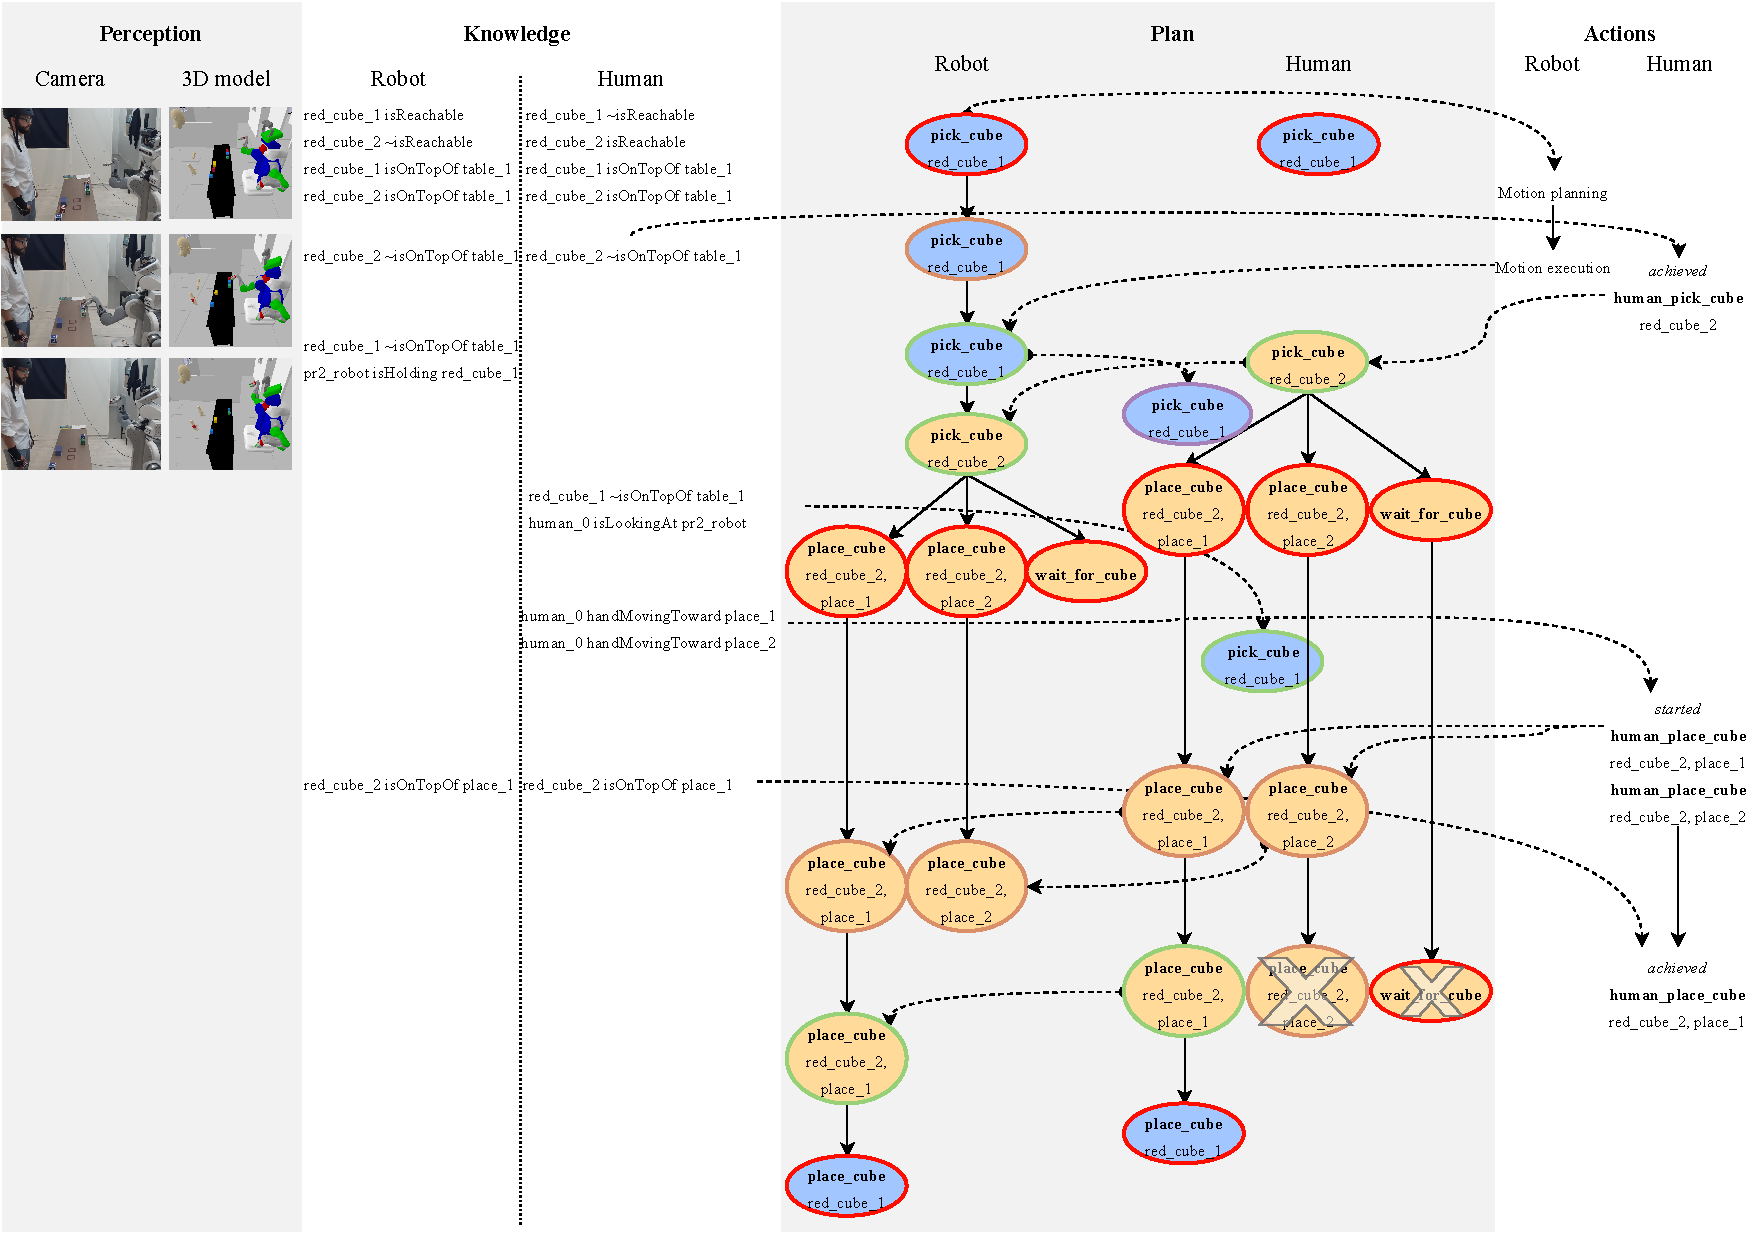
\includegraphics[width=0.9\linewidth]{figures/chapter2/debut_tache_deroule.pdf}
	\caption{Insight of what happens in the system during a collaborative task. Knowledge are facts generated by the Situation Assessment and Ontologenius. On one side there is the plan progress from the robot point of view (managed by the \acrshort{rpm}) and on the other side the plan progress from the human point of view, estimated by the robot (managed by the \acrshort{hpm}). The robot actions are sent by the \acrshort{aem} for execution to the Motion Planner and Executor. The human actions are recognized by the \acrshort{ham}.}
	\label{chap6:fig:debut_tache_deroule}
\end{figure}
\end{landscape}
\restoregeometry

\section{Conclusion and Future work}
In this chapter, we have proposed a generic supervision component providing robot decision and control to the robotic architecture it is integrated to, for collaborative robots. The developed \acrfull{rja} have their basis into the joint action principles presented in Chapter~\ref{chapter:chap1}. It endows the robot with knowledge representation, perspective-taking and \acrshort{tom}, joint attention, monitoring, communication, shared plan management. Have we respected the requirements listed in Chapter~\ref{chapter:chap4}?

\subsubsection*{How is it generic?}
First, the joint action and collaboration principles it tries to implement are valid in a certain number of collaborative contexts. Indeed, in any task, it is important to estimate the beliefs of the human partner, \ie what they perceive, what they know or not know of the task or the environment, and what they think of the task progress. Now, imagine a collaborative robot whose camera is on the chest and not its head. When performing a StackBuildingTask with the human, it could orient its head toward behind it, it would not matter for its own performance to the task. However, such a lack of joint attention would be prejudicial as contrary to what the human expects from a partner in a collaborative task. Then, to be able to monitor the human seems compulsory in order to what the robot partner does and so to be able to estimate the task progress and to act as well. And, Communication is also key. Indeed, who was not fed up with a virtual assistant which could not understand, at all, their request? Who wants to continue to interact with such device when it happens repeatedly? 

Then, the core of \acrshort{jahrvis} does not depend on a task. Every element that is task dependent is loaded in a separate file: action models, action recipes for execution and repair, and task goals. Facts to monitor human actions are automatically collected from the action models when starting the system and then it subscribes to them. For the rest, it is task-agnostic, the decision-making processes are task independent as the algorithms used are the same for different collaborative tasks (but of course it takes into account the task data in real-time as input). Indeed, to have \acrshort{jahrvis} manipulating a plan for a new task, the only condition is to respect the given format. Moreover, we presented \acrshort{jahrvis} running with two different task planners but if another planner with different characteristics was needed for a given task, it could be easily used as the only thing to do is to write the file to convert the plan into the write format and then to add it to the list of the known planners. Finally, the \acrshort{jahrvis} \acrshort{rja} themselves could be replace by other modules if respecting the format, such as the action recognition. Indeed, as well as the \acrlong{hpm} receives the lists of possibly started, ongoing or executed human actions, it is ``happy''.

\subsubsection*{How does it take the human partner into account?} First, \acrshort{jahrvis} bases itself on a robotic architecture incorporating human-aware components. The Situation Assessment computes two world representations: one for the robot and one for the human. Each of these worlds feeds the \acrlong{kb} corresponding to the given agent. It allows \acrshort{jahrvis} to make use of perspective-taking towards the human. Then, when performing a plan with the human, it tries to monitor them as often as possible. This allows to react consequently to the human's actions. Next, it has two separated processes to handle a shared plan in order to maintain an estimation of the human's knowledge about the task progress.

\subsubsection*{How does it leave decisions to the human?} Two methods were integrated to \acrshort{jahrvis} in order to have the robot flexible and adaptive. Indeed, to have a complete plan with all the object and agent actions allocated before even having started the task can be very limiting, as sometimes several objects can be possibly used to execute a given action for example. 

The first method was the use of an ``AgentX'' and object parameters under the form of \sparql{} queries. Thus, when an action is possible by either the human or the robot, or the human has the choice between two objects to act, the robot knows it and can adapt while considering it is normal. With a more classical plan, if the human took an appropriate object but not the one the robot had plan, re-planning would be needed and is not necessarily bad. But it leaves aside that the human did a choice that was making the plan progressing, and so that they were committed and not making errors.

The second method was the ability to handle conditional plans. The planner output a plan representing human choices at some points. Thus, \acrshort{jahrvis}, recognizing divergent plan branches, is aware when it has to wait for the human to make a choice. It monitors them and when it estimated the human chose a branch, it disables the other ones.

\subsubsection*{How does it recognize the human actions?} We showed that \acrshort{jahrvis} could successfully recognize human actions involving object manipulations, producing changes, new facts in the world. This feature is model based which is often not the case in other systems, as they use learning methods. Although being quite simple, it is very convenient to endow the robot with the ability to recognize a new action. Moreover, it is robust to unreliable perception, either because of the perception component or because the robot was not looking the human at the right time to observe them acting.

\subsubsection*{How does it handle contingencies?} Not so well. This is feature we wanted to explore at first, as explained in the thesis introduction. However, as we needed to have a system able to handle task in which everything was smooth, we implemented this first, leaving no time to develop nice strategies to handle contingencies and failures. However, we still implemented simple ways to react to such situations: when a human action is monitored and estimated as not being part of the plan, it replans, and when a robot action execution fails, it tries once again. If after the second tentative it still fails, it gives up the task, warning the human of its decision and its failure.

\subsubsection*{How does it manage relevant communications?} Dialog is not the focus of this thesis but it seemed important to us to think about communicative strategies that could be useful in task. We focused on the robot communicating about actions, either an action it executed or one that the human should perform. It was extensively based on the \acrshort{kb}s and the \acrfull{reg}, allowing to have nothing hard-coded except question prefixes. We also implemented an algorithm allowing the robot to parse a human order of an action to execute.

\subsubsection*{How does it consider interaction outside collaborative tasks?} We designed a frame, called interaction session, endowing the robot with internal states such a greetings, tasks, goodbyes. It is not developed much but it implements the minimum social rules of a social interaction: the greetings and the goodbyes. It also models that the robot can ``have a life of its own'' as not involved in an interaction session.

\subsubsection*{How does it adapt to human experience, abilities or preferences?} It was not the element on which we focused the most so the adaptation to the human abilities or preferences is poor or null in \acrshort{jahrvis}. However, this issue has been a bit tackled in the context of the direction-giving task presented in Chapter~\ref{chapter:chap8}. Moreover, we did not go really far in this direction but we investigated a bit the aspect concerning human experience, as \acrshort{jahrvis} feeds the \acrshort{kb}s with data about the collaborative task it is in. This allows the \acrshort{reg} to refer to past events when generating a referring expression on request of \acrshort{jahrvis}.



\ifdefined\included
\else
\bibliographystyle{acm}
\bibliography{These}
\end{document}
\fi


